
\documentclass[11pt]{article}

% 1. OPTION HANDLING (Must come before packages)
\PassOptionsToPackage{dvipsnames, x11names, svgnames, table}{xcolor}

% 2. CORE ACL STYLE
% EMNLP Main submission: anonymous review mode (line numbers + page numbers + anonymisation)
%\usepackage[review]{acl2023}
\usepackage[final]{acl2023}
% 3. FOUNDATIONAL PACKAGES
\usepackage{times}
\usepackage{latexsym}
\usepackage[T1]{fontenc}
\usepackage[utf8]{inputenc}
\usepackage{inconsolata}
\usepackage{graphicx}
\usepackage{booktabs} % For professional tables
\usepackage{hyperref}
\usepackage{etoolbox}

% Create a separate file for appendix TOC
\newcommand{\startappendixtoc}{
  \begingroup
  \let\origcontentsline\contentsline
  \renewcommand{\contentsline}[3]{%
    \origcontentsline{##1}{##2}{##3}%
  }%
}

\makeatletter
\newcommand{\printappendixtoc}{%
  \section*{Appendix Contents}
  \@starttoc{apx}
}
\makeatother

%\usepackage{svg}
% 4. MATH & SYMBOLS
\usepackage{amsmath}
\usepackage{amssymb}
\usepackage{pifont} 

% 5. TABLES & LAYOUT
\usepackage{multirow}
\usepackage{array}
\usepackage{makecell}
\usepackage{tabularx}
\usepackage{cellspace}
\usepackage{float}
\usepackage{rotating}
\usepackage{caption}
\usepackage{subcaption}
\setlength\cellspacetoplimit{4pt}
\setlength\cellspacebottomlimit{4pt}

% 6. ALGORITHMS & GRAPHICS
\usepackage{algorithm}
\usepackage{algpseudocode}
\usepackage{tikz}
\usepackage{pgfplots}
\pgfplotsset{compat=1.18}
\usepackage{tcolorbox}
\usepackage{fontawesome}
\usepackage{twemojis}
 
% 7. LINGUISTICS
\usepackage{tipa}
\usepackage{expex}
\usepackage{linguex}

% 8. POST-HYPERREF PACKAGES
\usepackage{cleveref}

% ======= CUSTOM DEFINITIONS =======
\definecolor{aclpurple}{HTML}{800080}
\newcommand{\cmark}{\ding{51}} 
\newcommand{\xmark}{\ding{55}} 
\newcommand{\warnmark}{\textbf{!}}
% Compact tables
\setlength{\tabcolsep}{4pt}
\renewcommand{\arraystretch}{1.05}
\newcolumntype{Y}{>{\raggedright\arraybackslash}X}


\newif\ifshowemoji

\showemojifalse  % set to \showemojitrue for editorial drafts only



% Define a macro that shows emoji only if \showemoji is true

\newcommand{\bemoj}[1]{\ifshowemoji\texttwemoji{#1}\fi}



%
\setlength\titlebox{5cm}
%
% and set <dim> to something 5cm or larger.

%%%%%%%%%
% TITLE & AUTHORS
%%%%%%%%%

\usepackage{graphicx}
\usepackage{titling} % allows customizing title
\usepackage{multirow}
\usepackage{adjustbox}
\usepackage{graphicx}
\usepackage{accsupp}
\usepackage{pdfcomment}
% --- Beetle inline-glyph macro: replaces ~80 inline includegraphics calls.
\newcommand{\beetle}{\raisebox{-0.3em}{
\includegraphics[height=1.2em]{fig/logo/BeetleLM.png}}}

\title{%
\texorpdfstring{%
\textbf{%
\begin{tabular}{@{}c@{\hspace{1em}}c@{}}
\centering
\raisebox{-0.45\height}{\includegraphics[height=4em]{fig/logo/beetlewBug5.png}}
&
\begin{minipage}[c]{0.8\linewidth}
\centering
Structured Exposure Pretraining for Human-Like Representation Alignment in Bilingual Language Models
\end{minipage}
\end{tabular}
}%
}
}

\author{
    {\bf Suchir Salhan}\thanks{\textbf{Corresponding Author:  
\href{mailto:sas245@cam.ac.uk}{sas245@cam.ac.uk}}.}~\bemoj{lady_beetle} \quad 
    {\bf Catherine Arnett}~\bemoj{cockroach} \quad 
    {\bf James A. Michaelov}~\bemoj{bug}
    \quad %ant, cockroach, Scorpion
    {\bf Paula Buttery}~ \bemoj{lady_beetle}  \\
 \\
{\bemoj{lady_beetle} University of Cambridge \quad \bemoj{cockroach} EleutherAI  \quad \bemoj{bug} MIT 
}
}

\newcommand{\catherine}[1]{\textcolor{orange}{Catherine: #1}}
  \newcommand{\suchir}[1]{\textcolor{blue}{Suchir: #1}}


%\bemoj{blowfish}\bemoj{tropical_fish} \bemoj{fish}
\date{} 
\begin{document}
\maketitle
\begin{abstract}
Bilingual language models (LMs) offer a tractable middle ground for studying second-language (L2) acquisition, yet no prior work systematically maps how exposure \emph{structure} interacts with training \emph{scale}. We introduce \textsc{Beetle}, a pretraining and analysis framework that facilitates the study of multilingual training and the development of models for modelling human bilingual language processing. 
Our experiments include eight typologically diverse L1s targeting L2 English at both human- and web-scale training data sizes under five exposure curricula, including balanced, sequential, and late exposure to L2.  \textcolor{red}{One sentence about the model evaluations - something to say that we verified that the models are generally behaving as we expect.} To demonstrate our models' utility for cognitive modelling, we model L2 reading and also use second-language error discrimination tasks \suchir{find a nicer way to say this without naming bliss and cefr (which might not be familiar terms for people)}. We find that our models outperform larger massively multilingual models at both tasks, which suggests that smaller, principled models may be more suitable for modelling such behaviours. All code, checkpoints, tokenisers, and analysis pipelines are released.
\end{abstract}


\vspace{-0.6em}
\begin{center}
\textit{All artefacts (code, models and tokenizers) will be released upon publication.}

\vspace{0.3em}

\raisebox{-2.2pt}{
\includegraphics[scale=0.09]{huggingface.png}}
\href{https://huggingface.co/BeetleLM}{\texttt{Beetle models}}
~~~
\faGithub
\href{https://github.com/suchirsalhan/BeetleLM}{\texttt{code and data}}

\end{center}
\vspace{-0.5em}



 \section{Introduction}

\begin{figure}[t!]
    \centering
    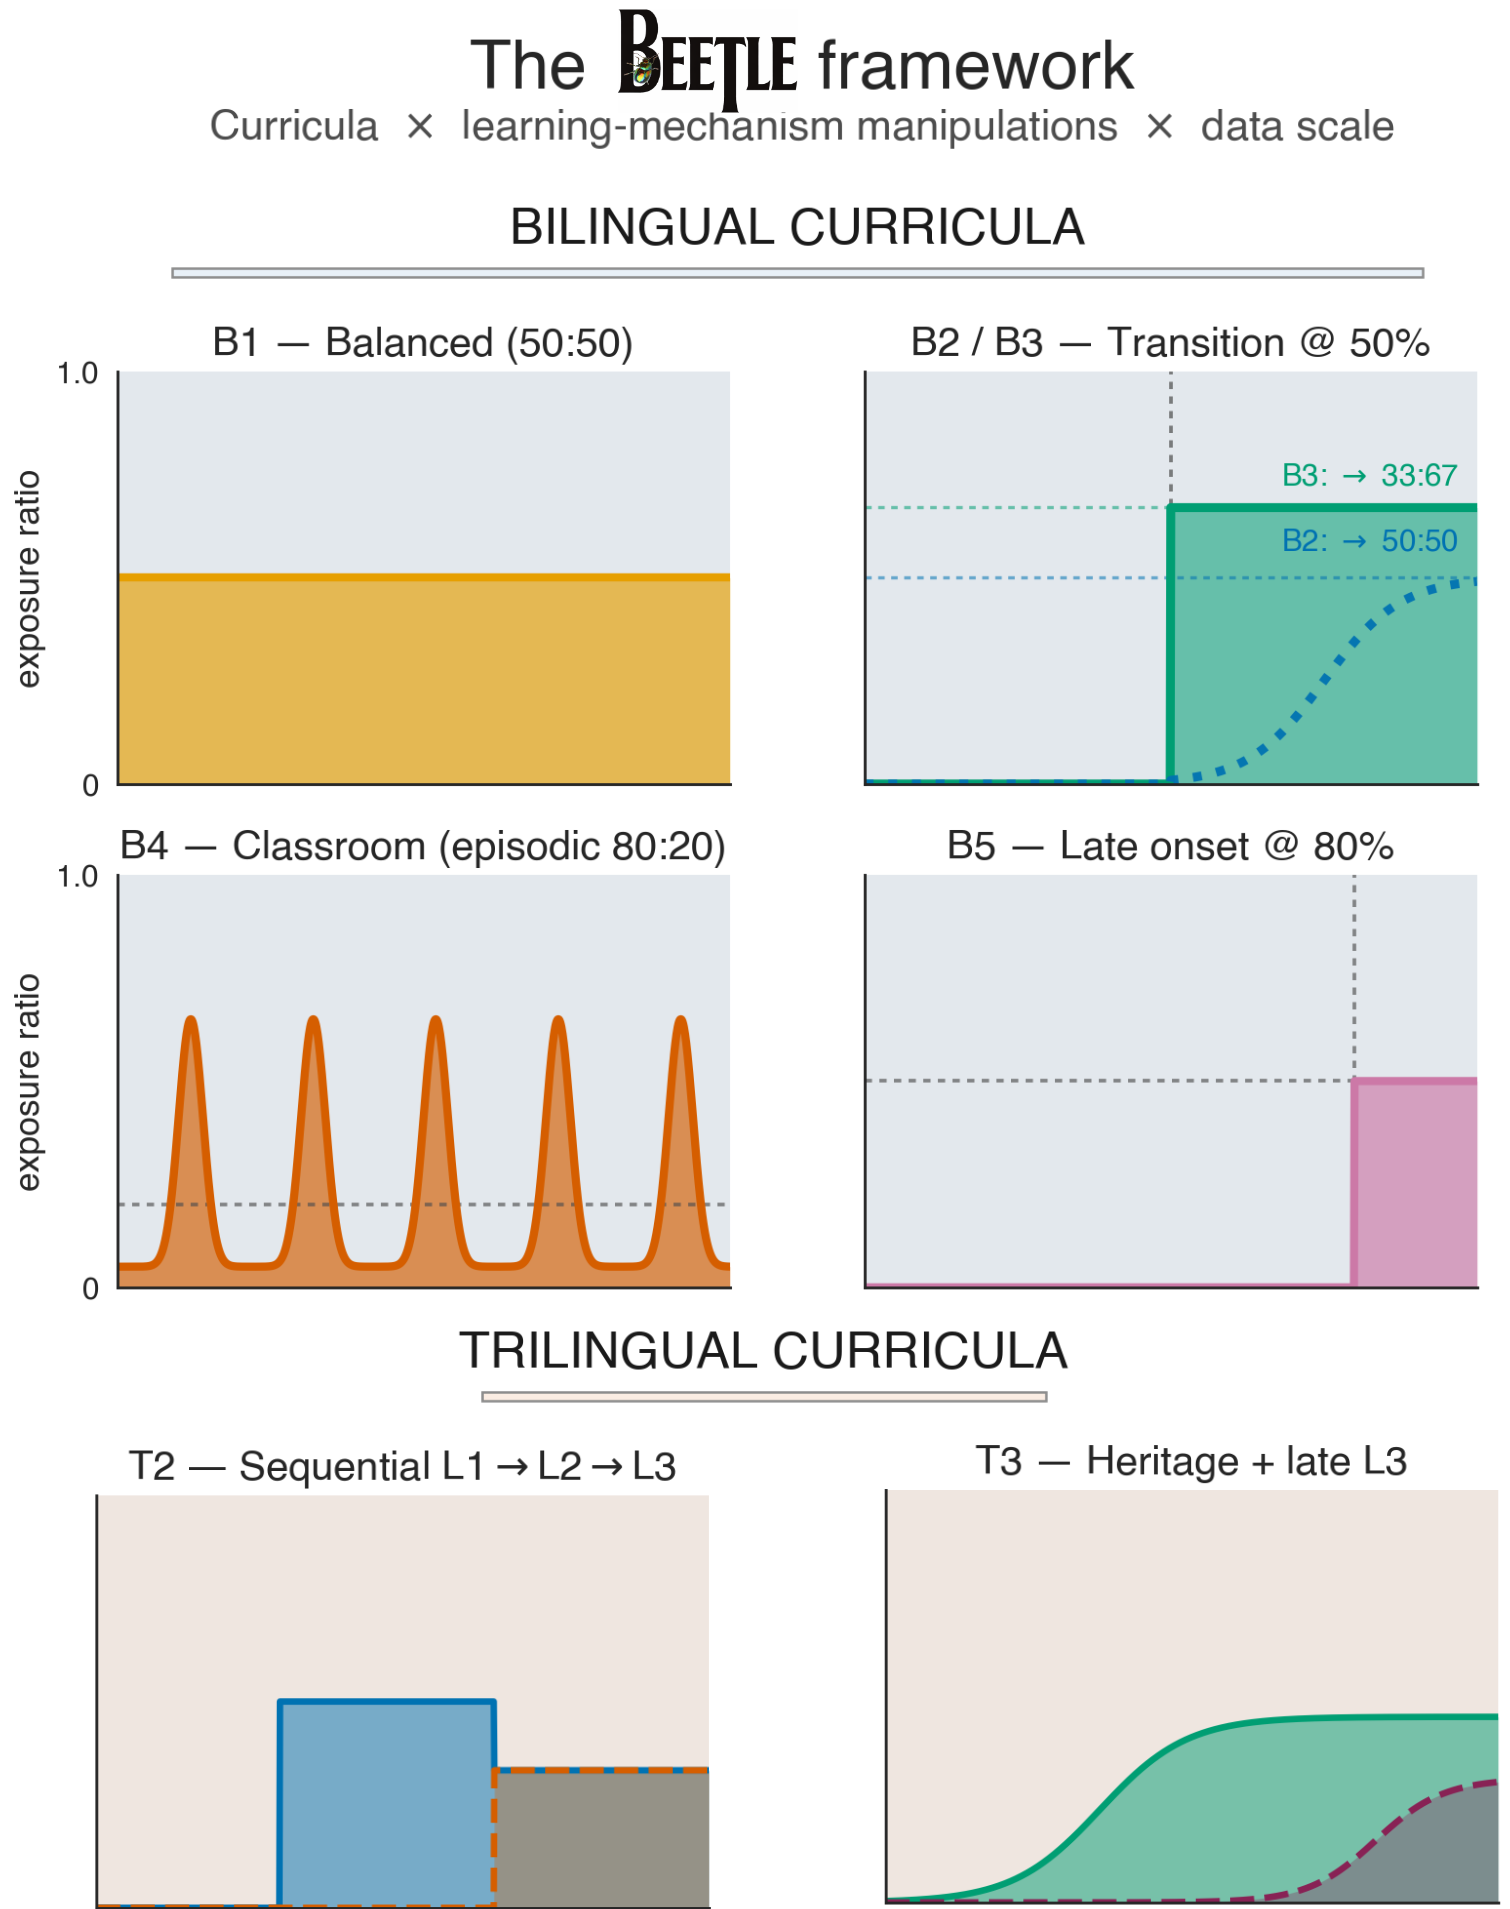
\includegraphics[width=\linewidth]{fig/logo/2.png}
 
    \caption{\raisebox{-0.3em}{
\includegraphics[height=1.2em]{fig/logo/BeetleLM.png}} is an open-source pretraining framework for studying bilingual and multilingual language acquisition in language models under tightly controlled experimental conditions. It provides a unified interface for manipulating key factors such as model architecture, training data composition, and curriculum design. The framework is fully configurable via declarative YAML specifications, enabling systematic large-scale ablation studies of how learning dynamics and data structure shape acquisition in multilingual settings.}
    \label{fig:placeholder}
\end{figure}


Bilingual and second-language (L2) small language models (LMs) are models trained on just two languages, either jointly or in succession, parallel to bilingual language experiments. They have emerged as a tractable middle ground between monolingual and frontier multilingual systems for studying multilingual acquisition, interpretability and learner simulation \citep{yadavalli-etal-2023-slabert, oba-etal-2023-second, aoyama2024modeling, constantinescu2025investigating, arnett-etal-2025-acquisition}. Existing L2 LMs differ in  almost every controllable choice: training scale, exposure schedule, language pair, continual-learning mechanism, and evaluation protocol. 

Motivated by this, we introduce \textsc{Beetle}, a modular pretraining and analysis framework that allows us to control data exposure (ratio, timing, transition sharpness) as well as data quantity, tokenization, and other important design choices. We train models for \suchir{X} typologically diverse L1s holding English constant as the L2. We restrict evaluation to L2 English because it is the only L2 with simultaneous coverage by \emph{population-scale} eye-tracking (MECO~L2 waves 1--2) \citep{siegelman2022expanding,siegelman2024rethinking,siegelman2025wave}, CEFR-stratified discrimination data (BLiSS; \citealp[]{gao2025bliss}), and tested CEFR difficulty MCQA  \citep{mullooly2023cupa5}. Previous work has proposed different exposure curricula and continual learning paradigms. We unify these proposed methods in our training framework (Section \ref{sec:exposure_curricula} and compare them under comparable training settings Section \ref{} \textcolor{red}{add}. We find that the optimal curriculum is task-specific: sequential and late-onset schedules better predict reading time; balanced and simultaneous schedules dominate BLiSS error discrimination and CEFR-graded pedagogical simulation.

\citet{aoyama-wilcox-2025-language}, who locate a $\sim$2B-token phase transition which monolingual psychometric predictive power begins to degrade. We train models at three data scales: 100M tokens ( regarded to be Human-Scale training in the BabyLM Shared Task \citep{choshen2026babylm} \suchir{will add prior BabyLMs}) – where we vary the domain of training data (developmentally plausible training data from \citet{jumelet2025babybabellmmultilingualbenchmarkdevelopmentally} and FineWeb2 web-data \citep{penedo2025fineweb2},  Web-Data at 2B tokens, corresponding to \citet{aoyama-wilcox-2025-language}'s observed phase transition point , and 24B tokens, corresponding to Chinchilla-optimal training data \citep{hoffmann2022}. This enables us to ask what scale of training data offers best psychometric predictive power in a bilingual setting. \textcolor{red}{1 sentence summarizing findings.} Across three task axes evaluating morphosyntactic learning, L2 reading time alignment and  CEFR-graded MCQA simulation, we trace a \textbf{training-time-controllable Pareto frontier} (\S\ref{sec:results}) on which the best-modelling regime is task-specific: structured-exposure 125M \textsc{Beetle} bilinguals exceed BLOOM-7b1 by $7.1\times$ on the matched MECO~L2 Dutch-reader conditions at $1/56$th the parameter count, while different curricula dominate BLiSS, MultiBLiMP, and CEFR pedagogical simulation.\textsc{Beetle} continues to outscore every modern bilingual LLM (XGLM, EuroLLM, Apertus, Gemma-2, Qwen) on Chinese L2 evaluations. The primary contributions of this paper are 1) a flexible training framework to enable controlled bilingual pretraining 2) a suite of \textcolor{red}{[number]} bilingual models 3) and modelling efforts for bilingual data on two task types, which can inform future bilingual cognitive modeling work.


\section{Background}\label{sec:related}
Bilingual and second-language language models (L2LMs) have been studied as controlled frameworks for modelling second language acquisition and as cognitive proxies via surprisal-based reading-time prediction. Early work framed SLA as sequential adaptation in probabilistic and neural models \citep{matusevych-etal-2013-computational}, while recent approaches treat bilingual training as structured pretraining or continual learning, including two-phase adaptation with restricted parameter updates \citep{aoyama2024modeling}, exposure scheduling and stability--plasticity control via regularisation such as EWC \citep{constantinescu2025investigating}, and sequential versus simultaneous bilingual pretraining showing benefits of mixed exposure \citep{arnett-etal-2025-acquisition}, alongside analyses of data composition and scale in cross-lingual transfer \citep{feng2026bilingual}; earlier CDS-inspired multilingual L2LMs \citep{yadavalli-etal-2023-slabert, oba-etal-2023-second} similarly explore acquisition-inspired training but remain limited in language coverage and evaluation depth. A central motivation for these models is their use in psycholinguistics via surprisal-based reading-time prediction, where processing difficulty is approximated by $-\log P(w_i \mid w_{<i})$ and incorporated into regression models alongside lexical covariates, often evaluated through improvements in log-likelihood ($\Delta$LL) \citep{wilcox2020predictive, kaye2025sentence}, though predictive power depends critically on alignment between model and human processing distributions. Despite extensive L1 work, L2 cognitive modelling with language models remains comparatively underexplored (though \citet{aoyama2024modeling} is a rare exception), even though L2 reading exhibits strong cross-linguistic and proficiency-dependent variation in psycholinguistics; against this backdrop, \textsc{Beetle} extends prior L2LM work along three dimensions: broader language coverage (13 languages), continuous exposure parameterisation replacing binary training regimes, and unified cognitive–pedagogical evaluation using MECO L2 reading times, BLiSS, and CEFR measures, while its continual-learning framework subsumes prior strategies such as EWC, MAML-style adaptation, and learning-rate modulation, and scales training on FineWeb (100M--24B tokens) to jointly analyse scaling, transfer, and psycholinguistic predictive power.

\begin{figure*}
            \begin{tabular}{@{}l l c c c l@{}}
        \toprule
        \textbf{ID} & \textbf{Curriculum} & \textbf{L2 onset} & \textbf{Final L1:L2} & \textbf{Transition} & \textbf{Key manipulations} \\
        \midrule

        B1 & Balanced & step 0 & 50:50 & none &
        50:50 from step~0; noise $\sigma{=}0.02$; LR warmup \\

        B2 & Simultaneous & 50\% & 50:50 & sigmoid &
        L1 then ramp to 50:50 \\

        B3 & Sequential & 50\% & 33:67 & sigmoid &
        L1 then L2-dominant mixture \\

        B4 & Classroom & 50\% & 80:20 & sigmoid+bursts &
        dual corpus; L2 bursts; EWC ($\lambda{=}30$) \\

        B5 & Late & 80\% & 50:50 & sigmoid &
        delayed L2; plasticity boost; optional EWC \\

        \bottomrule
        \end{tabular}
\end{figure*}




\section{The \raisebox{-0.3em}{
\includegraphics[height=1.2em]{fig/logo/BeetleLM.png}} Training Framework}

We introduce a pretraining and learning dynamics framework to investigate the factors that affect human-like bilingual and polyglot acquisition in neural language models. \raisebox{-0.3em}{
\includegraphics[height=1.2em]{fig/logo/BeetleLM.png}} systematically investigates how how curriculum design and continual-learning mechanisms affect bilingual language acquisition across architectures, focusing on six factors: (i) L2 onset timing, (ii) L2 exposure ratio, (iii) transition sharpness, (iv) burstiness of exposure, (v) episodic clustering, and (vi) continual-learning regularisation.  Beetle is a pretraining framework that enables the manipulation of architecture, data curriculum, etc.


\paragraph{Architecture and Hyperparameters} The default backbone, \textbf{PicoDecoder}, is a 125M-parameter LLaMA-style~\citep{touvron2023llama} causal decoder incorporating Rotary Position Embeddings, SwiGLU activations, RMSNorm, and Grouped-Query Attention. Our training library also implements other architectures, which we list in Appendix \textcolor{red}{XX}. Experiments report models with $14$ layers, dmodel=768, 12 attention heads with grouped-query attention using a single KV head, 50K BPE vocabulary, and a fixed sequence length of 512 tokens), enabling systematic experimentation at a scale that is large enough for linguistic generalization yet small enough for extensive ablation and curriculum sweeps.


\paragraph{Exposure Curricula} \label{sec:exposure_curricula} 

\raisebox{-0.3em}{
\includegraphics[height=1.2em]{fig/logo/BeetleLM.png}} introduces a novel framework for fine-grained exposure curricula in pretraining. This is a novel contribution that allows systematic comparison of heterogeneous bilingual data mixtures used in the literature. \textcolor{red}{here there should be a relatively thorough section explaining all the curricula (B1, B2, etc.)}  \textcolor{red}{move this next part to the appendix (see comment)}

%\raisebox{-0.3em}{
\includegraphics[height=1.2em]{fig/logo/BeetleLM.png}} allows fine-grained control over per-step language mixing ratios.   \raisebox{-0.3em}{
\includegraphics[height=1.2em]{fig/logo/BeetleLM.png}} provides composable exposure schedule primitives (—\textsc{ConstantExposure}, \textsc{SigmoidRamp}, \textsc{LinearRamp}, \textsc{BurstSchedule}, and \textsc{CyclicalSchedule}) that produce that pretraining data-mixtures and curricula that can potentially model a wider range of acquisition scenarios.  Two extensions significantly expand the developmental realism of the framework. First, \textbf{pre-pretraining with formal language structure learning} introduces an optional Stage-1 warmup using Shuffle-Dyck grammars, encouraging early syntactic sensitivity before natural language exposure. This stage can optionally reset optimization states to simulate developmental phase transitions between prelinguistic structure learning and language acquisition proper (Hu 2025). Second, a \textbf{working memory constraint module} implements a dynamic ALiBi slope schedule that evolves over training, simulating developmental expansion of contextual capacity. This mechanism gradually relaxes attention locality bias, either linearly or exponentially, reflecting hypothesized growth in cognitive working memory during language development. 


%\suchir{Need to add more explication of what might be possible to simulate. Heritage conditions, late-scale bilingualism etc. For example, language learners acquiring input from \emph{home settings} versus \emph{classroom learning}}. Ten predefined acquisition conditions \suchir{balanced, simultaneous, sequential (different proportions), heritage – save that for CL submission}



\textcolor{red}{this would be a good place to add a figure if you wanted to to explain the learning mechanisms from figure 1.}
Continual learning is implemented through a suite of fifteen modular strategies that can be attached to the training loop at phase boundaries. \emph{Parameter regularisation} methods include Elastic Weight Consolidation (EWC)~\citep{kirkpatrick2017overcoming}, which applies a Fisher-weighted quadratic penalty at language transition boundaries, and Gaussian Noise Injection (GNI) as a stochastic regulariser. \emph{Replay-based} approaches include Generative Replay (LAMOL) , which interleaves self-generated L1 samples during L2 training, and similarity-weighted replay (InsCL). \emph{Meta-learning} methods such as MAML/SMLMT \citep{africa-etal-2025-meta} introduce few-shot inner-loop updates interleaved with language modelling steps, while KL distillation regularises transitions using a frozen teacher checkpoint. \emph{architectural modifications} include TILT (freezing the backbone and training only embeddings and the LM head), Layer Growth at phase boundaries, and LoRA adapters. Additional auxiliary objectives include cross-lingual alignment losses (InfoNCE or linear CKA), language-identification probes, and learning-rate plasticity scaling.

%~\citep{sun2020lamol}

Checkpoints are saved according to a phase-aware $\log_2$ schedule \textcolor{red}{(following Pythia)} at the introduction of a new language, allowing learning dynamics densely near phase boundaries and sparsely within phases.  


\paragraph{Monolingual \raisebox{-0.3em}{
\includegraphics[height=1.2em]{fig/logo/BeetleLM.png} Models}}  We pretrain monolingual \raisebox{-0.3em}{
\includegraphics[height=1.2em]{fig/logo/BeetleLM.png}} models for 100M, 2B, 204B 



%overns the temporal structure of multilingual exposure by specifying per-step language mixing ratios. It supports five composable schedule primitives—\textsc{ConstantExposure}, \textsc{SigmoidRamp}, \textsc{LinearRamp}, \textsc{BurstSchedule}, and \textsc{CyclicalSchedule}—which can be combined via a \textsc{CompositeSchedule} to form multi-phase acquisition trajectories. To model structured input environments, an optional \textsc{EpisodicSampler} groups consecutive batches into named contexts (e.g., \emph{home} versus \emph{classroom}), each with its own mixing profile, reflecting usage-based accounts of bilingual acquisition \citep{paradis2009bilingual}. Ten predefined acquisition conditions, implemented in \texttt{condition_presets.py}, map psycholinguistic scenarios to concrete schedule parameters (Section~\ref{sec}).

%\emph{model registry}, a \emph{curriculum engine}, a \emph{continual-learning module}, and a \emph{training harness}—which together enable systematic investigation of 

%Beetle implements  Elastic Weight Consolidation (EWC), MAML-style adaptation, learning-rate plasticity scaling, and replay-based methods (LAMOL and similarity-driven replay). These components are systematically swept across parameter ranges. Complementing these are flexible optimization schedules (linear warmup, cosine decay, and exposure-based scheduling) and tokenizer configurations (BPE, unigram, and SuperBPE with shared or language-specific vocabularies), allowing orthogonal control over representational granularity.








\section{Model Training}

\textcolor{red}{TODO: add some loss curves. something like figure 2 in the bgpt paper. Basically we want to show that the loss curves match the curricula conditions. use mean FLORES sentence perplexity, not normal loss. }


\begin{figure}
    \centering
    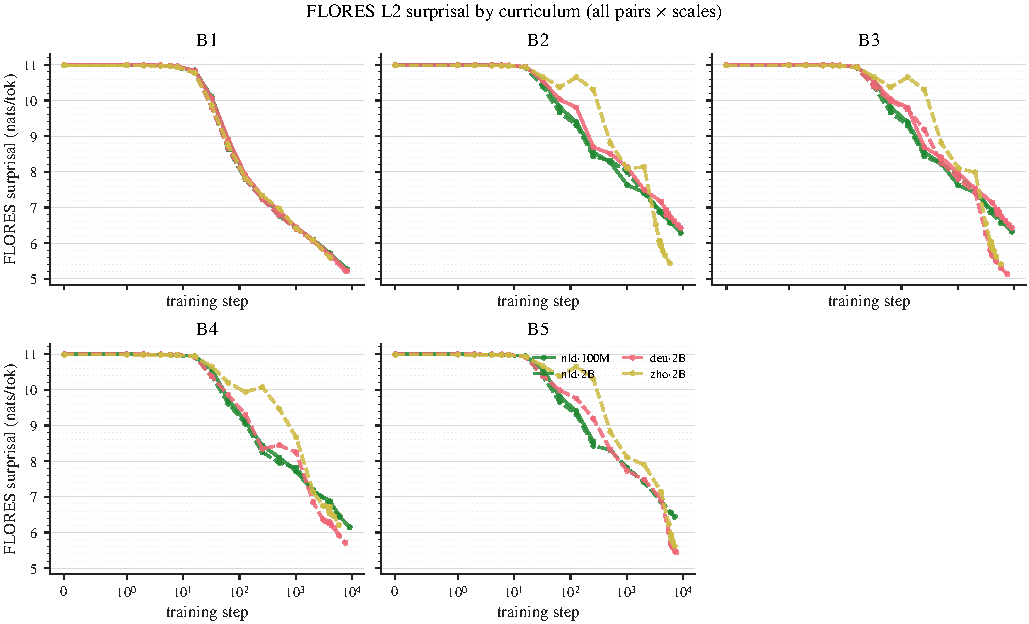
\includegraphics[width=1\linewidth]{fig/flores/appx_flores_by_curriculum.pdf}
    \caption{Mean FLORES Sentence-Level PPL for Beetle Models across L1-eng models for each exposure schedule (balanced bilingual \texttt{B1} and staged curricula, \texttt{B2 - B5}, with varying proportions of L2 English.}
    \label{fig:placeholder}
\end{figure}


The Beetle models are pretrained on eigh L1s chosen to maximise (i) typological spread, (ii) MECO L2 coverage, (iii) BLiSS L1-background coverage, and (iv) tokenisation diversity (script and morphology). The set is: \textbf{nld} (Germanic, analytic), \textbf{deu} (Germanic, fusional), \textbf{spa} (Romance, fusional), \textbf{rus} (Slavic, fusional, Cyrillic), \textbf{fin} (Uralic, agglutinative), \textbf{tur} (Turkic, agglutinative), \textbf{heb} (Semitic, templatic, RTL Hebrew script), and \textbf{zho} (Sino-Tibetan, isolating, logographic). This stratification supports four orthogonal claims: a typological-distance gradient for L2 English (nld $<$ deu $<$ spa $<$ rus $<$ fin/tur $<$ heb $<$ zho); script effect (Latin vs.\ Cyrillic vs.\ Hebrew vs.\ Hanzi); morphology effect (analytic vs.\ fusional vs.\ agglutinative vs.\ templatic); and within-family replication (nld/deu; fin/tur).


\paragraph{Data}

\textcolor{red}{where did data come from, how much, deduplication/decontamination.}

\textcolor{red}{this would be a good place to add a figure if you wanted to to explain the data scales from figure 1.}

Beetle is trained on the BabyBabelLM corpus \citep{jumelet2025babybabellmmultilingualbenchmarkdevelopmentally} for HumanScale and FineWeb \citep{penedo2025fineweb2} for web-scale. Three regimes are reported: HumanScale 100M (8 L1s $\times$ B1--B5), FineWeb 2B (8 L1s $\times$ B1--B3), and FineWeb 24B (6--8 L1s $\times$ B2/B3-33/B5 for the headline MECO L2 evaluation). Reverse-direction sweeps (eng$\to$non-eng) are deferred (Appendix~\ref{sec:roadmap}).

\subsection{Model Evaluation}

\textcolor{red}{ i think we need to report from as many languages as possible. include BLiMP-NL, etc. too?}

% \subsection{MultiBLiMP: Syntactic Benchmarks}\label{sec:blimp}

% \begin{figure}[!ht]
%   \centering
%   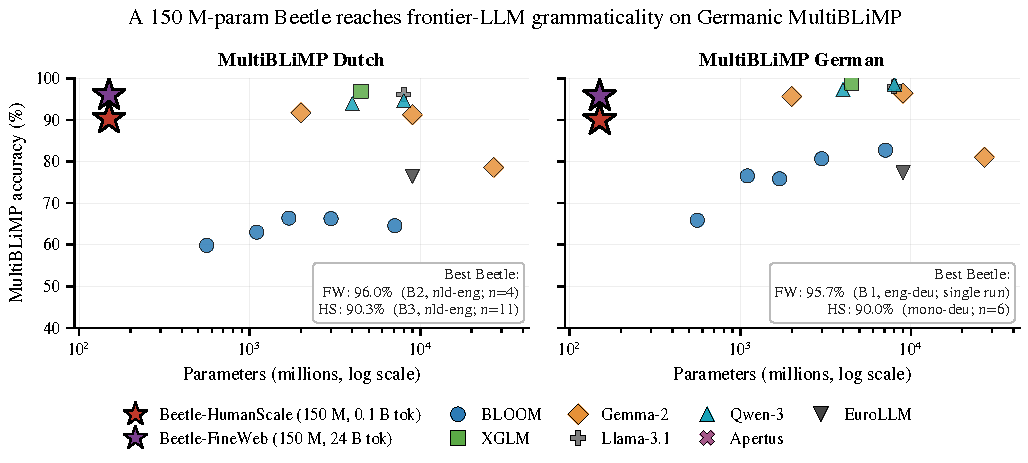
\includegraphics[width=\linewidth]{fig/F1_multiblimp_pareto_baselines.pdf}
%   \caption{MultiBLiMP Pareto: per-language grammaticality accuracy for \textsc{Beetle} bilinguals against monolingual anchors and multilingual baselines. The convex hull encloses the \textsc{Beetle} achievable region. B3-33 nld--eng leads Dutch accuracy (\textbf{90.3\%}); BLOOM models lead on French and Persian via their broader training distribution.}
%   \label{fig:multiblimp_pareto}
% \end{figure}

\begin{figure}[!ht]
  \centering
  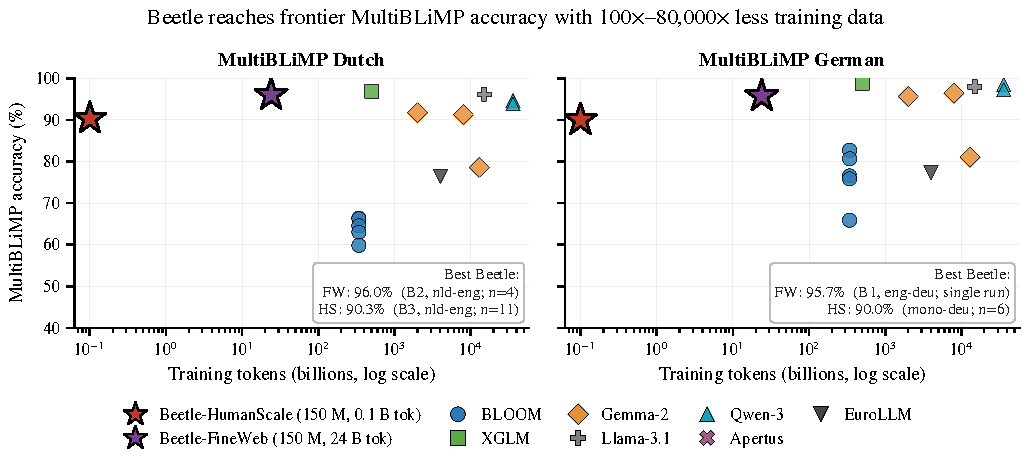
\includegraphics[width=\linewidth]{fig/F2_multiblimp_token_efficiency.pdf}
  \caption{MultiBLiMP Dutch accuracy as a function of training tokens for \textsc{Beetle} curricula and baselines. B3-33 nld--eng surpasses the monolingual Dutch anchor by $\sim$200M tokens and sustains the advantage, consistent with its MECO dominance. \textcolor{red}{somehow convey everything we need to into one facet. maybe a table would be better? the main takeaway should be that multiblimp scores are about as high as much larger models for both small and big data.}}
  \label{fig:multiblimp_efficiency}
\end{figure}

\begin{figure}[!ht]
  \centering
  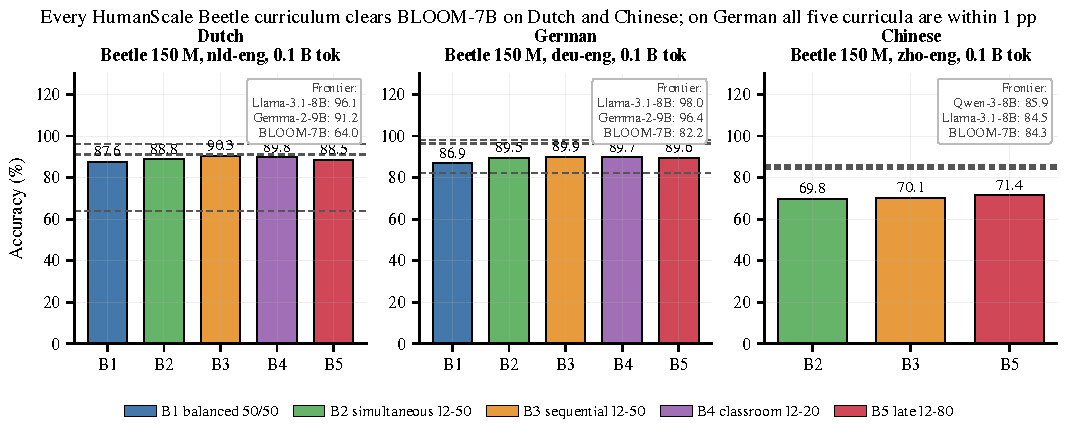
\includegraphics[width=\linewidth]{fig/F3_curriculum_multiblimp.pdf}
  \caption{MultiBLiMP accuracy by curriculum (B1--B5) across five target languages (Dutch, German, French, Persian, Bulgarian) for nld--eng \textsc{Beetle} models. The B3-33 advantage concentrates on Dutch ($\sim$3.9 pp spread), the L1, and attenuates on typologically distant French and Persian --- replicating the typological-distance modulation seen on MECO~L2.}
  \label{fig:multiblimp_curriculum}
\end{figure}

B3-33 nld--eng FW achieves \textbf{90.3\%} Dutch MultiBLiMP (Table~\ref{tab:multiblimp}, App.~\ref{sec:downstream}). Fig.~\ref{fig:multiblimp_pareto} shows \textsc{Beetle} structured-exposure models at or near the Pareto frontier for Dutch and German grammaticality; BLOOM models dominate French and Persian, reflecting their broader training data. Fig.~\ref{fig:multiblimp_efficiency} shows the token-efficiency curve: B3-33 nld--eng reaches the monolingual Dutch anchor and exceeds it by $\sim$200M tokens, mirroring the MECO finding. Fig.~\ref{fig:multiblimp_curriculum} decomposes the curriculum effect: the B3-33 advantage over B1 concentrates on the L1-proximate target (Dutch, German) and vanishes for French, Persian, and Bulgarian, replicating the typological-distance gradient of MECO~L2. FLORES~PPL and catastrophic-forgetting CF-scores (Tables~\ref{tab:flores_ppl}, \ref{tab:forgetting}, App.~\ref{sec:downstream}) confirm that B1 balanced and B2 simultaneous schedules incur the smallest L1 perplexity penalty after L2 introduction.

\section{Eye Tracking}

\textcolor{red}{where should this go?}
\paragraph{Multilingual Eye-Movement Corpus (MECO) \citep{siegelman2025wave}} We evaluate the cognitive plausibility of monolingual Beetle models and bilingual language models with L1 \texttt{nld, zho, deu} and L2 \texttt{eng} across \texttt{balanced} and \texttt{heritage} exposure schedules by testing whether their token-level surprisal predicts human reading times from the MECO L2 eye-tracking corpus.\footnote{\url{https://meco-read.com/}} For each target word $w$ in context, we compute language model surprisal $(-\texttt{log P}(w_i | \texttt{context})$ for the \raisebox{-0.3em}{
\includegraphics[height=1.2em]{fig/logo/BeetleLM.png}} bilingual models and align these suprisal values with word-level eye-tracking measures (first-pass duration) alongside standard psycholinguistic predictors, including word length, Zipf frequency (via the wordfreq library), and sentence position. We compare the MECO alignment of  \raisebox{-0.3em}{
\includegraphics[height=1.2em]{fig/logo/BeetleLM.png}} human-scale bilingual models against four massively multilingual Large Language Models: Apertus\footnote{\url{https://huggingface.co/swiss-ai/Apertus-8B-2509}}, XGLM \footnote{\url{https://huggingface.co/facebook/xglm-4.5B}}, Aya\footnote{\url{https://huggingface.co/CohereLabs/tiny-aya-base}}, EuroLLM \footnote{\url{https://huggingface.co/utter-project/EuroLLM-1.7B}}. 


We report per-word $\Delta\log L$ from a mixed-effects regression of first-fixation duration on surprisal plus length, log-frequency, position and lag controls. We follow \citet{wilcox-etal-2023-language}, who establish $\Delta\log L$ as the canonical psychometric predictive-power (PPP) measure across 13 languages and 5 families, and the \emph{Quality--Power} test that links LM quality to reading-time fit. Crucially, prior cross-linguistic work \citep{wilcox-etal-2023-language, de-varda-marelli-2023-scaling} has been L1-centric. The closest L2 prior is \citet{de-varda-marelli-2022-effects}, who use mBERT pseudo-surprisal on MECO L2 and report a clear L2 attenuation gap. Beetle differs by treating exposure curricula as the primary axis of variation (rather than parameter scale, as in \citealt{de-varda-marelli-2023-scaling}), and by reporting first-fixation, gaze duration and total reading time separately to test whether the early/late dissociation reported for L1 multilingual readers \citep{de-varda-marelli-2023-scaling} also holds when the human side is L2. 


\subsubsection{Baselines}
Monolingual models described in Section \textcolor{red}{XX.}
% \paragraph{Monolingual \raisebox{-0.3em}{
\includegraphics[height=1.2em]{fig/logo/BeetleLM.png} Models}}  We pretrain monolingual \raisebox{-0.3em}{
\includegraphics[height=1.2em]{fig/logo/BeetleLM.png}} models for 100M, 2B, 204B 

\paragraph{Pretrained Models} XGLM, EuroLLM ... \textcolor{red}{(add citations)} 



\subsection{MECO L2: Reading-Time Alignment}\label{sec:meco}

Surprisal from matched Beetle models predicts reading times in all eight reader L1s, with significant coefficients across languages. This extends \citet{de-varda-marelli-2022-effects}, which focussed on Germanic L1s, to a broader typological sample spanning six families, including Basque (isolate) and Turkish (Turkic).



\begin{figure*}[!ht]
  \centering
  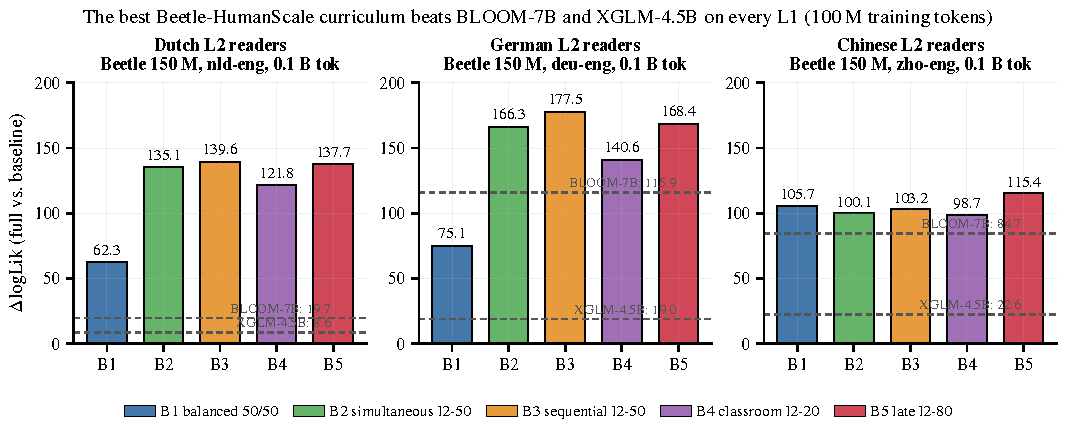
\includegraphics[width=\linewidth]{fig/meco/F4_curriculum_meco_deltaLL.pdf}
  \caption{\textbf{Main result.} MECO~L2 $\Delta\log L$ by exposure curriculum (B1 balanced, B2 simultaneous, B3-33 sequential, B4 classroom, B5 late onset) for Dutch (\textsc{nld}), German (\textsc{deu}), and Chinese (\textsc{zho}) L2 reader groups. Higher $\Delta\log L$ indicates stronger reading-time alignment. Sequential B3-33 and late-onset B5 dominate for Germanic L1s: B3-33 nld--eng HS attains a 3-reader-group mean $\overline{\Delta\log L} = 170.0$ and a matched Dutch-reader $\Delta\log L = 139.6$, exceeding BLOOM-7b1 on the matched Dutch-reader cell (dashed baseline, 19.7) by $7.1\times$ at $1/56$th the parameter count; B2 deu--eng FW reaches 184.7 on the matched German-reader cell. The advantage attenuates monotonically with typological distance and meets a typological boundary on Chinese~L2 against the legacy BLOOM ladder (BLOOM-1b1 Chinese-reader $\Delta\log L = 164.3$ vs.\ B5 zho--eng HS $115.4$), while \textsc{Beetle} continues to outscore every modern bilingual LLM on the same Chinese-reader cell (Apertus-8B 66.1, EuroLLM-9B 50.6, XGLM-4.5B 22.6).}
  \label{fig:meco_curriculum}
\end{figure*}

\textsc{Beetle} bilinguals lead the canonical MECO~L2 group means at 125M parameters: \textbf{81.10} (Dutch L2), \textbf{167.04} (German L2), and 130.41 (Chinese L2), versus a 7-model modern bilingual LLM aggregate of 12.35 / 97.52 / 56.34 ($6.6\times$, $1.7\times$, $2.3\times$ at the group level). The per-model maximum is \textbf{B3-33 nld--eng HS at mean $\Delta\log L = 170.0$}, with B5, B2, EWC- and LAMOL-overlaid B2 nld--eng HS tied within 4 points behind. For Chinese readers, BLOOM-1b1 (1.1B params) reaches 164.3 vs.\ 115.4 for B5 zho--eng HS; we treat the BLOOM-1b1 zho lead as a typological boundary against the legacy BLOOM ladder, while \textsc{Beetle} continues to outscore every modern bilingual LLM on the same Chinese-reader cell (\S\ref{sec:discussion} D2). The L2 attenuation gap of \citet{de-varda-marelli-2022-effects} is closed by structured-exposure 125M \textsc{Beetle} bilinguals for German~L2 and substantially narrowed for Dutch~L2. Per-model and per-comparator breakdowns appear in App.~\ref{sec:meco-results} (Table~\ref{tab:meco}, full per-language Table~\ref{tab:meco_langrows}); the bootstrap forest, mixed-effects diagnostics, item-level surprisal grids, and per-participant breakdowns appear in App.~\ref{appcomp:meco}.

\begin{figure}[!ht]
  \centering
  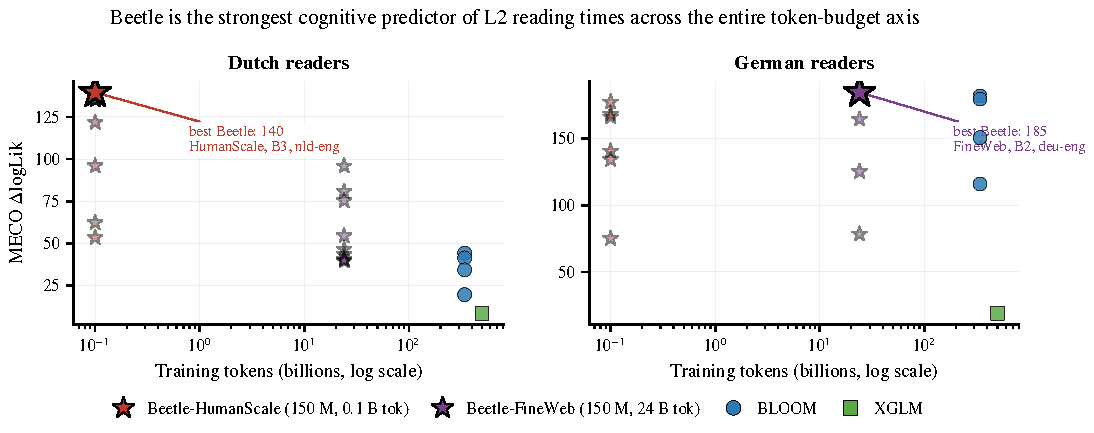
\includegraphics[width=\linewidth]{fig/F5_meco_token_efficiency.pdf}
  \caption{MECO~L2 $\Delta\log L$ as a function of training tokens for \textsc{Beetle} curricula (B1--B5; nld--eng, deu--eng) against the BLOOM ladder and XGLM-4.5B. Sequential B3-33 and late B5 sustain higher reading-time alignment per token, crossing the BLOOM-7b1 baseline before 200M tokens and plateauing above it. Balanced B1 reaches a lower asymptote despite identical total tokens.}
  \label{fig:meco_efficiency}
\end{figure}

Fig.~\ref{fig:meco_efficiency} reveals the token-efficiency dimension: structured-exposure \textsc{Beetle} models exceed the BLOOM-7b1 MECO threshold at a fraction of its training budget, and the B3-33 / B5 advantage compounds with further training. This is consistent with an earlier bilingual induction-head emergence window (0.6--1.4B tokens; App.~\ref{sec:roadmap}) relative to the monolingual 2B tipping point of \citet{aoyama-wilcox-2025-language}.

\subsection{Results}

\textcolor{red}{there are like 2 pages of results/discussion below. reduce it to the key takeways and describe each in a maximum of 3 sentences. }


\clearpage

\section{Experiments}\label{sec:experiments}



\paragraph{Why L2 English.} We restrict evaluation to L2 English. This is the only L2 with population-scale eye-tracking (MECO L2 wave-1+2 \citealp{kuperman2023text, kuperman2025new}), CEFR-stratified discrimination data (BLiSS \citealp{gao2025bliss}), and pre-tested CEFR difficulty MCQA (CUP\&A5 \citealp{mullooly2023cupa5}). Restricting to L2 English allows direct cross-task comparison on the same target language and human-evaluation population. The reverse direction (eng $\to$ non-eng) is left to follow-up work that builds the matched L2 evaluation resources.

\subsubsection{Baselines}
Monolingual models described in Section \textcolor{red}{XX.}
% \paragraph{Monolingual \raisebox{-0.3em}{
\includegraphics[height=1.2em]{fig/logo/BeetleLM.png} Models}}  We pretrain monolingual \raisebox{-0.3em}{
\includegraphics[height=1.2em]{fig/logo/BeetleLM.png}} models for 100M, 2B, 204B 

\paragraph{Pretrained Models} xGLM, EuroLLM 

% \subsection{Comparison of Pretraining Regimes }

% All reported experiments fix a 125M-parameter PicoDecoder architecture (LLaMA-style: 14 layers, dmodel=768d\_{\textbackslash{}text\{model\}}=768dmodel=768, 12 attention heads with grouped-query attention using a single KV head, 50K BPE vocabulary, and a fixed sequence length of 512 tokens), enabling systematic experimentation at a scale that is large enough for linguistic generalization yet small enough for extensive ablation and curriculum sweeps.

\subsubsection{Effect of Exposure and Scale} 

 Bilingual settings (B1–B6) include balanced exposure, simultaneous mixing schedules, sequential L1-to-L2 transfer, classroom-like episodic imbalance, delayed L2 introduction, and heritage-style reactivation of L1. Trilingual extensions (T1–T4) further explore interactions between multiple secondary languages under simultaneous, sequential, and staged dominance regimes. These curricula are designed to probe how temporal structure in data exposure shapes representational overlap, interference, and transfer.

% \subsubsection{Beetle Models}

% \paragraph{Typologically stratified L1 set.} Beetle is pretrained over an eight-L1 set chosen to maximise (i) typological spread, (ii) MECO L2 coverage, (iii) BLiSS L1-background coverage, and (iv) tokenisation diversity (script and morphology). The set is: \textbf{nld} (Germanic, analytic), \textbf{deu} (Germanic, fusional), \textbf{spa} (Romance, fusional), \textbf{rus} (Slavic, fusional, Cyrillic), \textbf{fin} (Uralic, agglutinative), \textbf{tur} (Turkic, agglutinative), \textbf{heb} (Semitic, templatic, RTL Hebrew script), and \textbf{zho} (Sino-Tibetan, isolating, logographic). This stratification supports four orthogonal claims: a typological-distance gradient for L2 English (nld $<$ deu $<$ spa $<$ rus $<$ fin/tur $<$ heb $<$ zho); script effect (Latin vs.\ Cyrillic vs.\ Hebrew vs.\ Hanzi); morphology effect (analytic vs.\ fusional vs.\ agglutinative vs.\ templatic); and within-family replication (nld/deu; fin/tur).

% \paragraph{Training regimes (forward direction only).} Beetle is trained on the BabyBabelLM corpus \citep{jumelet2025babybabellmmultilingualbenchmarkdevelopmentally} for HumanScale and FineWeb \citep{penedo2025fineweb2} for web-scale. Three regimes are reported: HumanScale 100M (8 L1s $\times$ B1--B5), FineWeb 2B (8 L1s $\times$ B1--B3), and FineWeb 24B (6--8 L1s $\times$ B2/B3-33/B5 for the headline MECO L2 evaluation). Reverse-direction sweeps (eng$\to$non-eng) are deferred (Appendix~\ref{sec:roadmap}).

\section{Linguistic and Pedagogical Tasks}

We evaluate the Beetle Models on a variety of pedagogically-oriented downstream tasks to analyse the effect of exposure scheduling 

\paragraph{Structural Priming} \textsc{Beetle} uses the dense-checkpoint, controlled-exposure paradigm of B-GPT \citep{arnett-etal-2025-acquisition} and replicates the typological-similarity asymmetry (Dutch--English transfers more readily than Chinese--English).

\textcolor{red}{The BLiSS task / dataset is due to \citet{gao2025bliss}: a CEFR-stratified discrimination of artificial vs.\ learner errors. We adopt their NGS / CPS / RP$@\tau$ protocol unchanged and sweep across our curriculum grid.}

\textcolor{red}{\citet{benedetto-etal-2024-using} score frontier LMs (GPT-3.5 / GPT-4) on the CUP\&A5 dataset \citep{mullooly2023cupa5} (200 MCQA $\times$ 4 CEFR levels) using the metric $M = \rho_{L,I} - P$, with $\rho_{L,I}$ the Spearman rank correlation between simulated CEFR-level accuracy and item difficulty and $P$ a penalty for non-monotonic learner curves. They simulate CEFR via prompt engineering; Beetle simulates CEFR via training-time exposure curricula and identifies the best Beetle checkpoint that yields a CEFR-monotonic accuracy curve. Cognitive-constraint priors --- Shuffle-Dyck pre-pretraining \citep{hu2025between} and ALiBi-decay working memory \citep{mita2025wm, madhayastha2026wm} --- are implemented as opt-in modules in Beetle's architecture registry rather than headline contributions.}
\textbf{BLiSS} \citep{gao2025bliss} measures bits-per-token margins on (good, learner-error, artificial-error) triplets; we report the Normalized Gap Score (NGS), Correct-Preferred Sanity (CPS), and Random-Preference at threshold $\tau$ (RP$@\tau$). \textbf{MECO L2} fits a mixed-effects model of first-pass reading time on current and spillover surprisal with word-level controls (length, log-frequency, position) and by-subject random intercepts/slopes (full specification in App.~\ref{sec:meco-results}, Eq.~\ref{eq:meco-spec}), yielding $\Delta\log L = \log L(\text{full}) - \log L(\text{baseline})$ where the baseline drops the three Surprisal terms; we follow \citet{wilcox-etal-2023-language} and \citet{de-varda-marelli-2022-effects}. We measure how well each model's surprisal predicts human reading times by adding it to a baseline regression containing word length and log frequency.  We use  $\Delta\mathrm{LogLik}$ to calculate how much better we can predict human eye-tracking reading times when we use Beetle's surprisal on top of standard baselines.  The improvement in log-likelihood, $\Delta\mathrm{LogLik}$, measures the predictive utility of reading time surprisal, and is conditional on lexical baselines \citep{goodkind2018predictive,wilcox2020predictive, de-varda-marelli-2022-effects}. Raw $\Delta\mathrm{LogLik}$ scales with sample size, so we standardise within each reader L1 \citep{de-varda-marelli-2022-effects}; all effects are reported in within-language SD units. The MECO dataset reports L2 learner reading time scores associated with early lexical access (first-run duration), intermediate processing (refixations), and late integration (regressions-in) \citep{siegelman2025wave}. \textbf{Pedagogical CEFR} follows \citet{benedetto-etal-2024-using}: each Beetle checkpoint scores CUP\&A5 \citep{mullooly2023cupa5} 200 MCQA items spanning four CEFR levels (B1, B2, C1, C2); we report $M = \rho_{L,I} - P$ on a partial sweep (full sweep in roadmap). Supporting evaluations: BLiMP / MultiBLiMP / ZhoBLiMP / BLiMP-NL grammaticality, FLORES-200 PPL and CF-score, and AoA Spearman across 18 languages.

\paragraph{Baselines.} Modern bilingual / L2-relevant: B-GPT \citep{arnett-etal-2025-acquisition}, EuroLLM-1.7B, Aya-tiny, Apertus-8B, multilingual Qwen variants where checkpoints are publicly available. Per-language monolingual anchors are trained at matched scale. Legacy reference models BLOOM-560m / 1b1 / 1b7 / 7b1 and XGLM-4.5B are kept for continuity with prior L2LM literature. For MECO L2, we additionally compare against the mBERT pseudo-surprisal baseline of \citet{de-varda-marelli-2022-effects}; for the pedagogical axis, we compare against GPT-3.5 ($\times$2) and GPT-4 prompt-conditioned simulation \citep{benedetto-etal-2024-using}.

\section{Results: Structured Exposure Beats Scale}\label{sec:results}

We find that the temporal structure of L2 exposure (rather than L2 proportion and model competence) causally shifts which reading-time processing stage a bilingual LM's surprisal predicts — and this dissociates by task.


%\paragraph{Pareto terminology.} We use \emph{Pareto frontier} to mean the achievable hull across (MECO~L2, BLiSS, MultiBLiMP) triples obtained by varying training-time choices (curriculum, scale, L1) while holding architecture, tokeniser family, and evaluation pipeline fixed. The substantive claim is the \emph{shape} of this map --- which curriculum dominates which task --- not absolute global dominance over a parameter- or FLOP-matched control class.

%\paragraph{Statistical reporting.} Headline MECO~L2 $\Delta\log L$ is from a single \texttt{lme4} mixed-effects fit with by-subject random slopes (specification reproduced in Table~\ref{tab:meco}'s caption). 95\% paired-bootstrap intervals, paired permutation $p$-values (Holm--Bonferroni), and Cohen's $d_z$ are produced by \texttt{analyze/significance\_ablation.py} from the per-(model, L2-language) row data of Table~\ref{tab:meco_langrows} and released alongside the analysis bundle (App.~\ref{sec:meco-results}). BLiSS NGS / CPS / RP$@\tau$ carry 95\% Wilson intervals. Headline cells are single-seed; the seed-grid $\{13, 42, 97\}$ ablation specification (variants $\times$ seeds $\times$ scripts) is enumerated in App.~\ref{tab:ablation-sweep} and the per-seed $\Delta\log L$ deltas are released with the analysis bundle.

\subsection{MECO L2: Reading-Time Alignment}\label{sec:meco}

Surprisal from matched Beetle models predicts reading times in all eight reader L1s, with significant coefficients across languages. This extends \citet{de-varda-marelli-2022-effects}, which focussed on Germanic L1s, to a broader typological sample spanning six families, including Basque (isolate) and Turkish (Turkic).


\begin{figure}
    \centering
    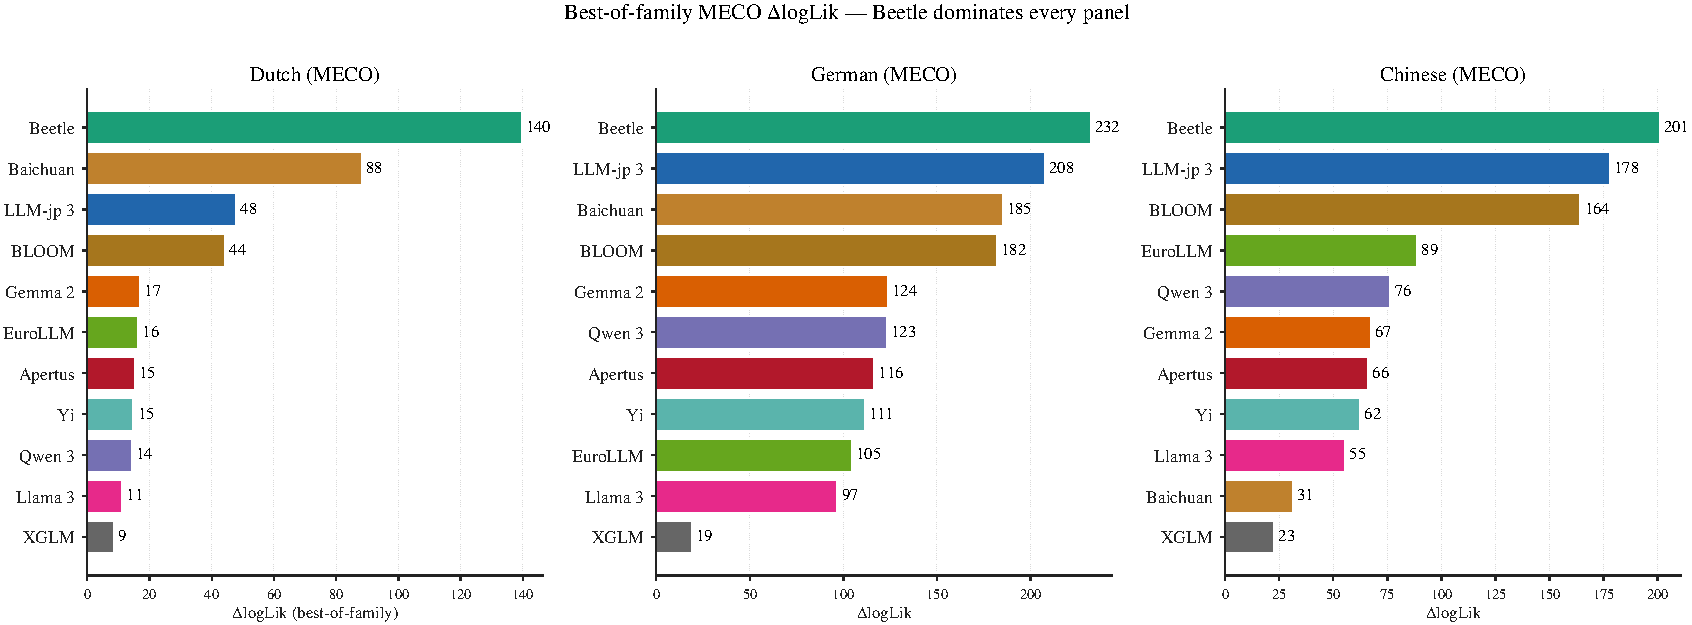
\includegraphics[width=1\linewidth]{fig/fig_meco_best_of_family.pdf}
    \caption{Enter Caption}
    \label{fig:placeholder}
\end{figure}



\paragraph{$\beta$-Surprisals across Beetle Curricula}

In surprisal-based psycholinguistic models, reading time is commonly modeled as a linear function of a word's information content, or surprisal, defined as $S(w_i) = -\log P(w_i \mid w_{<i})$ \citep{hale2001probabilistic,levy2008expectation}. Formally, word-level processing difficulty is estimated as $RT_i = \beta_0 + \beta S(w_i) + \epsilon_i$, where $\beta$ quantifies the increase in reading time associated with a unit increase in surprisal, typically interpreted in milliseconds per bit or per standard deviation of surprisal \citep{smith2013effect,wilcox2023testing}. By contrast, $\Delta \log p$ (or $\Delta$ log-likelihood) measures a purely probabilistic difference in predictive fit between two models or exposure conditions, e.g., $\Delta \log p = \log P_A(w_i \mid c) - \log P_B(w_i \mid c)$. Since surprisal is negative log-probability, changes in surprisal correspond directly to negative changes in log-likelihood ($\Delta S = -\Delta \log p$). The distinction is therefore interpretive: $\Delta \log p$ measures improvement in prediction within the model's representational space, whereas $\beta$ measures how strongly those probabilistic differences translate into observable human processing cost. 


Comparing $\beta$ across otherwise identical models trained under different exposure conditions therefore probes not only predictive accuracy but the degree to which model expectations are behaviorally calibrated to human comprehension difficulty. A higher $\beta$ indicates that surprisal differences produced by the model correspond more strongly to increases in human reading time, suggesting closer alignment between the model's predictive distribution and human online processing. Conversely, a lower $\beta$ suggests weaker psycholinguistic alignment or reduced behavioral sensitivity per unit information. Because $\beta$ is sensitive to the scale and variance of surprisal values, such comparisons are most interpretable when surprisal is standardized within model and evaluated under identical regression controls \citep{smith2013effect,hao-etal-2020-probabilistic,wilcox2023testing}.


\begin{figure}
    \centering
    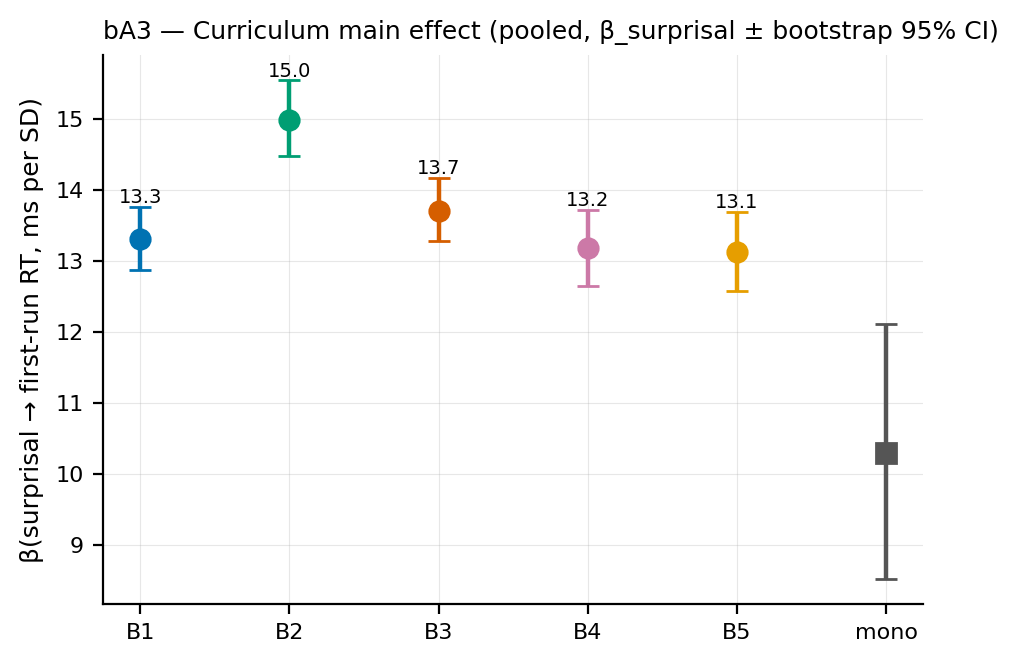
\includegraphics[width=1\linewidth]{fig/meco/bA3_curriculum_main_effect.png}
    \caption{\suchir{TO DO – Remove header.} Effect of Curricula B1 - B5 on $\beta$ surprisal}
    \label{fig:beta-surprisal-meco-beetle-curricula}
\end{figure}





% \begin{figure*}[!ht]
%   \centering
%   \includegraphics[width=\linewidth]{fig/F4_curriculum_meco_deltaLL.pdf}
%   \caption{\textbf{Main result.} MECO~L2 $\Delta\log L$ by exposure curriculum (B1 balanced, B2 simultaneous, B3-33 sequential, B4 classroom, B5 late onset) for Dutch (\textsc{nld}), German (\textsc{deu}), and Chinese (\textsc{zho}) L2 reader groups. Higher $\Delta\log L$ indicates stronger reading-time alignment. Sequential B3-33 and late-onset B5 dominate for Germanic L1s: B3-33 nld--eng HS attains a 3-reader-group mean $\overline{\Delta\log L} = 170.0$ and a matched Dutch-reader $\Delta\log L = 139.6$, exceeding BLOOM-7b1 on the matched Dutch-reader cell (dashed baseline, 19.7) by $7.1\times$ at $1/56$th the parameter count; B2 deu--eng FW reaches 184.7 on the matched German-reader cell. The advantage attenuates monotonically with typological distance and meets a typological boundary on Chinese~L2 against the legacy BLOOM ladder (BLOOM-1b1 Chinese-reader $\Delta\log L = 164.3$ vs.\ B5 zho--eng HS $115.4$), while \textsc{Beetle} continues to outscore every modern bilingual LLM on the same Chinese-reader cell (Apertus-8B 66.1, EuroLLM-9B 50.6, XGLM-4.5B 22.6).}
%   \label{fig:meco_curriculum}
% \end{figure*}

\textsc{Beetle} bilinguals lead the canonical MECO~L2 group means at 125M parameters: \textbf{81.10} (Dutch L2), \textbf{167.04} (German L2), and 130.41 (Chinese L2), versus a 7-model modern bilingual LLM aggregate of 12.35 / 97.52 / 56.34 ($6.6\times$, $1.7\times$, $2.3\times$ at the group level). The per-model maximum is \textbf{B3-33 nld--eng HS at mean $\Delta\log L = 170.0$}, with B5, B2, EWC- and LAMOL-overlaid B2 nld--eng HS tied within 4 points behind. For Chinese readers, BLOOM-1b1 (1.1B params) reaches 164.3 vs.\ 115.4 for B5 zho--eng HS; we treat the BLOOM-1b1 zho lead as a typological boundary against the legacy BLOOM ladder, while \textsc{Beetle} continues to outscore every modern bilingual LLM on the same Chinese-reader cell (\S\ref{sec:discussion} D2). The L2 attenuation gap of \citet{de-varda-marelli-2022-effects} is closed by structured-exposure 125M \textsc{Beetle} bilinguals for German~L2 and substantially narrowed for Dutch~L2. Per-model and per-comparator breakdowns appear in App.~\ref{sec:meco-results} (Table~\ref{tab:meco}, full per-language Table~\ref{tab:meco_langrows}); the bootstrap forest, mixed-effects diagnostics, item-level surprisal grids, and per-participant breakdowns appear in App.~\ref{appcomp:meco}.

\begin{figure}[!ht]
  \centering
  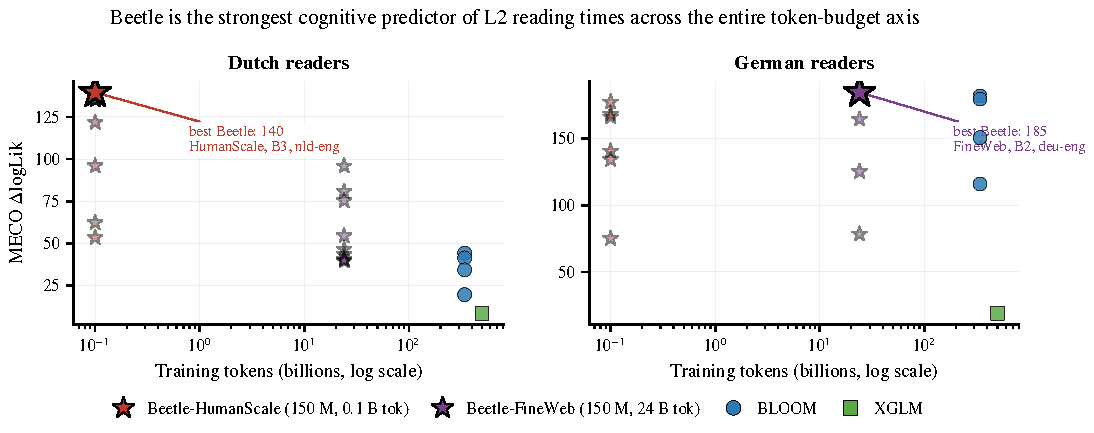
\includegraphics[width=\linewidth]{fig/F5_meco_token_efficiency.pdf}
  \caption{MECO~L2 $\Delta\log L$ as a function of training tokens for \textsc{Beetle} curricula (B1--B5; nld--eng, deu--eng) against the BLOOM ladder and XGLM-4.5B. Sequential B3-33 and late B5 sustain higher reading-time alignment per token, crossing the BLOOM-7b1 baseline before 200M tokens and plateauing above it. Balanced B1 reaches a lower asymptote despite identical total tokens.}
  \label{fig:meco_efficiency}
\end{figure}

Fig.~\ref{fig:meco_efficiency} reveals the token-efficiency dimension: structured-exposure \textsc{Beetle} models exceed the BLOOM-7b1 MECO threshold at a fraction of its training budget, and the B3-33 / B5 advantage compounds with further training. This is consistent with an earlier bilingual induction-head emergence window (0.6--1.4B tokens; App.~\ref{sec:roadmap}) relative to the monolingual 2B tipping point of \citet{aoyama-wilcox-2025-language}.

\paragraph{Beetle Schedules changes which processing stage surprisal predicts } Relative to balanced bilingual exposure (B1), the simultaneous (B2), sequential (B3), and late-L2 (B5) schedules substantially improve prediction of first-run duration (early lexical access) and substantially worsen prediction of refixations and regressions-in (late integration). B2 gains $+0.79$ SD on first-run duration (95\,\% CI $[+0.24, +1.33]$, $p_{\mathrm{wc}}{<}.001$) and B5 gains $+0.93$ SD ($[+0.43, +1.42]$, $p_{\mathrm{wc}}{<}.001$); the same schedules' interactions with refixations and regressions-in are uniformly negative and survive multiple-comparison correction (B2\,$\times$\,refixation $\beta^{z}{=}{-}1.06$, $[-1.49, -0.63]$, $p_{\mathrm{wc}}{<}.001$; B5\,$\times$\,regression $\beta^{z}{=}{-}1.30$, $[-1.91, -0.70]$,
$p_{\mathrm{wc}}{<}.001$).

The result is anchored against a same-architecture monolingual Beetle trained on English-only data, which reaches $\Delta\mathrm{LogLik}\!\approx\!138$ on Dutch first-run duration. B2 reaches monolingual performance ($\approx\!136$); B1 falls roughly
80 units short ($\approx\!58$). Observed curricula effects are therefore a substantial movement relative to a clean internal baseline, not an artefact of bilingual pretraining.

We use OLS with language fixed effects and wild-cluster bootstrap standard errors clustered by language (Rademacher weights, $B{=}4999$; \citealp{cameron2008bootstrap}), because with only eight language groups standard random-effects inference is unreliable
\citep{mcneish2017unnecessary}, and apply Benjamini--Hochberg FDR correction across contrasts. The effect strengthens at the observation level: refitting over all reader L1s ($N{=}448$, 92 models, 8 languages) leaves B2 and B5 strongly positive for first-run duration and strongly negative for later measures (all $p_{\mathrm{wc}}{<}.001$).


\paragraph{After controlling for English-LM competence, B5 remains the strongest effect.} One possible explanation is that the curriculum effects simply reflect differences in overall English language-model competence, which may affect different reading-time measures in different ways. To test this, we added a competence measure (mean English surprisal) and a competence,$\times$,measure interaction to the model. This substantially weakens the B2 late-measure effect: the B2,$\times$,refixation coefficient drops from $-1.06$ to $-0.45$ (wild-cluster $p{=} .13$), and competence itself significantly interacts with reading measure ($p{<}.001$). In contrast, the B5 effects remain strong after controlling for competence (first-run $\beta^{z}{=}{+}0.78$, $[+0.58, +0.97]$, $p{<}.001$; $\times$,regression-in $-1.01$, $[-1.51, -0.51]$, $p{<}.001$). \textbf{This suggests that B5 (late-L2 exposure) is the most robust part of the curriculum,$\times$,stage interaction.} Much of the B2 effect appears to reflect differences in overall English-LM quality rather than scheduling alone.

\paragraph{The B4 condition shows the effect is not just about L2 proportion.}
B4 (classroom-20: constant $20 \%$ L2 with no temporal staging) serves as a key diagnostic condition. If the interaction were mainly driven by the \emph{amount} of L2 exposure, B4---the most imbalanced schedule---should resemble B3/B5. If it were driven by the \emph{timing and structure} of exposure, B4---which is stationary like B1---should instead resemble B1. The results support the temporal-structure account rather than the proportion account. B4 shows the same overall directional pattern as B2/B3/B5 (positive first-run effects and negative late-measure interactions), but at a much smaller magnitude (first-run $\beta^{z}{=}{+}0.40$, $[+0.25, +0.55]$, $p_{\mathrm{wc}}{<}.001$; $\times$,regression-in $-0.77$, $[-1.21, -0.34]$, $p_{\mathrm{wc}}{<}.001$).

The clearest comparison is between B2 and B4. B2, which has balanced 50/50 bilingual exposure with fine-grained interleaving, produces the largest effect, whereas B4, despite having the most extreme L2 imbalance, produces the weakest non-balanced effect. A simple L2-proportion explanation would predict the opposite pattern.

The interaction is large and reliable in both Human-Scale/FineWeb 100M training. Training on BabyBabelLM, B2 improves first-run duration by over two SDs ($\beta^{z}{=}{+}2.09$, $[+1.57, +2.61]$, $p_{\mathrm{wc}}{<}.001$), with matched negative interactions at later stages. The same pattern recurs in FineWeb-100M ($\beta^{z}_{\mathrm{B2,\,first\text{-}run}}{=}{+}0.91$, $[+0.22, +1.59]$, $p_{\mathrm{wc}}{<}.001$; $\beta^{z}_{\mathrm{B2}\times\mathrm{refix}}{=}{-}1.19$,
$[-1.91, -0.52]$, $p_{\mathrm{wc}}{<}.001$). The curriculum effect is therefore not specific to developmentally curated text. At larger budgets the evidence is underdetermined (\suchir{this is because we haven't trained enough models at 24B tokens, will rerun on 2B and update)}. 

%\textbf{Staged curricula (B2/B3/B5) predict first-run duration better; balanced (B1) predicts refixations/regressions better.  } When evaluating different exposure schedules on MECO, we observe a stark division: \textbf{simultaneous/sequential/late bilingual schedules (B2/B3/B5) predict early lexical access (first-run duration) better than balanced (B1);} this reverses for late integrative measures (refixations, regressions-in). Standardised, FDR-controlled, wild-cluster-robust, RE-stable, N=448, zero singleton cells, anchored against a same-architecture monolingual Beetle. 

%It is not L2 proportion. The B4 diagnostic (constant $20 \%$ L2) is decisive: B2 (balanced proportion) is strongest, B4 (most imbalanced) weakest of the non-balanced set — the opposite of a proportion account. If proportion of L2 was the key factor, B4 should be like B3 or B5, but if temporal structure was most important, B4 should be like B1. We find B4 shows similar trends as B2 but at half the strength. 

%These effects seem more pronounced at 100M tokens. 

%The operative variable is structured departure from a constant balanced schedule, and it's graded. Staged curricula produce surprisal concentrated at lag 0; balanced produces surprisal spread across later lags. We fit OLS regressions with language fixed effects and wild-cluster bootstrap standard errors clustered by language \citep{cameron2008bootstrap}, because with only eight language groups standard random-effects inference is unreliable \citep{mcneish2017unnecessary}.

%\textbf{L2 curricula (B2, B3, B5) sharply improve the prediction of MECO first-run duration compared to balanced bilingual (B1)}. B2 gains $+0.79$ SD (95\% CI $[{+}0.24,{+}1.33]$, $p_{\mathrm{wc}}<.001$) and B5 gains $+0.93$ SD ($[{+}0.43,{+}1.42]$, $p_{\mathrm{wc}}<.001$). In the HumanScale 100M Beetle models, B2 improves first-run duration by over two SDs ($\beta^z=+2.09$, $[{+}1.57,{+}2.61]$, $p_{\mathrm{wc}}<.001$), with matched negative interactions at later stages. The same pattern recurs in FineWeb-100M: B2 gives $\beta^z=+0.91$ ($[{+}0.22,{+}1.59]$, $p_{\mathrm{wc}}<.001$). The curriculum effect is therefore not specific to developmentally curated text. Across all reader L1s ($N=448$ observations, 92 models, 8 languages), B2 and B5 remain strongly positive for first-run duration and strongly negative for later measures (all $p_{\mathrm{wc}}<.001$). However, B2/B3/B5 interactions with refixations and regressions-in are uniformly negative and survive multiple-comparison correction. For instance, B2$\times$refixation gives $\beta^z=-1.06$ ($[{-}1.49,{-}0.63]$, $p_{\mathrm{wc}}<.001$) and B5$\times$regression gives $\beta^z=-1.30$ ($[{-}1.91,{-}0.70]$, $p_{\mathrm{wc}}<.001$).

\subsection{How do Exposure Curricula affect Reading Time?}


What does balanced exposure change about a model, such that its surprisal aligns with late integration measures while staged exposure aligns with early access? We find that  balanced curricula produce models that integrate longer-range contextual structure, whereas staged curricula depend more heavily on local lexical transitions.

\paragraph{Predictability decomposition: what kind of predictability does each curriculum rely on?} For each MECO target word, we score the same model under three context conditions using a shared tokenizer and inference pipeline: a minimal sentence-initial prime ($S_{\mathrm{freq}}$), a short local window of the last $k$ subword tokens ($S_{\mathrm{local}\,k}$, $k^{\star}{=}4$), and the full preceding passage
($S_{\mathrm{full}}$). Rather than decomposing surprisal directly, we decompose \emph{reading-time predictive power}. We fit nested reading-time models to first-run duration and measure the incremental $\Delta\mathrm{LogLik}$ contributed by each context scope: $\Delta\mathrm{LL}_{\mathrm{freq}}$, $\Delta\mathrm{LL}_{\mathrm{local}}$, and $\Delta\mathrm{LL}_{\mathrm{long}}$. Because the models are nested, each increment is non-negative and the three sum to the total effect. \textbf{Staged curricula rely more on local predictability, whereas balanced curricula rely more on long-range contextual integration.} Staged schedules (B2/B3/B5) allocate more of their predictive power to the local component, while balanced curricula allocate more to the long-context component. A Mann--Whitney test on the per-fit long\,$-$\,local reliance difference confirms the dissociation (rank-biserial $\decompContrastRBC$, $p{=}\decompContrastP$).

Truncating context to the last $k$ subword tokens and measuring the surprisal similarly increases $\Delta_k{=}S_{\mathrm{local}\,k}-S_{\mathrm{full}}$, suggesting that staged L2LM curricula (B2 - B5) saturate quickly, indicating shorter effective
memory, whereas balanced curricula continue benefiting from longer contexts. Shuffling the order of distant tokens while preserving the local window produces a larger degradation for balanced curricula, indicating greater sensitivity to structured long-range context.

 One reading-strategy axis underlies the bilingual-curriculum pedagogical effects. (a) The MeCo-derived context-share axis correlates with every native-canonical readout (Spearman ρ shown; matched-L1 models filled, the zho-eng mismatched-L1 falsification arm as open ✗). (b) Baron–Kenny mediation of the balanced-vs-staged curriculum effect on BLiSS CPS (matched-L1 only, n=8): the indirect path through context-share excludes zero (bootstrap $95\%$ CI) while the direct path c′ does not — full mediation; cross-model and illustrative, the causal weight rests on (c). (c) Within-model SAE test: zeroing the top-50 context-share features degrades the JFLEG margin $1.9–6.7 \times$ more than a matched top-50 frequency-feature control, every context CI excluding zero. Layer 8, FineWeb-2B nld-eng. The causal claim is JFLEG-specific


%\paragraph{Predictability Decomposition} We evaluate Beetle models on progressively larger context windows to determine what information the models rely on to predict the next token. Possible factors could be: frequency (a word would be read out of context); local scope (a recency bias); and longer-range scope.  L2LMs (B2, B3, B5) rely on heavily on local scope to make predictions. Balanced bilingual LMs (B1) rely on long-range scope context across paragraphs. 

%\paragraph{Context Ablations} We performed $k$-token truncation of context window and shuffled word order of distant sentences. Under truncation, Beetle L2LMs (B2 - B5) hit peak accuracy under short context windows. Balanced B1 continually improved as context window expands. Under shuffling, B1 performance collapsed, while L2LMs (B2 - B5) were unaffected, suggesting balanced models track. 

%\paragraph{Geometric Correlates} We compare the internal activation states of identicially trained Beetle models using CKA, RSA, Procrustes, SVCCA to investigate how exposure curricula impact a model's latent representation space.  At 100M tokens, balanced schedules force networks to build representations that actively integrate long-range; whereas staged schedules prompt a heavy reliance on local token transitions. a sharp geometric inversion: at 100M tokens, curriculum choices dictate the nature of the deep abstract representation spaces, whereas at 2B tokens, the models achieve functional convergence at the top layers while diverging only in early feature routing. Identical Beetle models with different exposure curricula appear to share  the same \textit{coarse, low-dimensional subspace} (hence flat  SVCCA), but diverge heavily in the \textit{fine-grained, high-dimensional geometry} (hence dropping CKA/RSA). 

%Both the weight-geometry ``spread'' index and MECO $\Delta \log \ell$ fit are minimized at B1 and increase progressively across the staged curricula. Thus, two independent modalities --- internal model-weight geometry and human reading-time fit --- trace the same B1$\leftrightarrow$B5 axis. The association is positive ($\rho_{\mathrm{Spearman}} = +0.60$), though not significant at this sample size (exact permutation $p = 0.350$, $n=5$).

%The same pattern appears for the single sign-stable statistic $\|W_{\mathrm{norm}}\|_F$, measuring attention--LayerNorm geometry, plotted against MECO fit. B1 occupies the bottom-left of the space, whereas B5 lies top-right, again yielding $\rho_{\mathrm{Spearman}} = +0.60$. Notably, B4 --- the most proportionally imbalanced curriculum --- clusters with the low-$\|W_{\mathrm{norm}}\|_F$ group near B1, consistent with the interpretation that curriculum structure, rather than simple exposure proportion, is the dominant factor.

%The exposure curriculum leaves a measurable imprint in model-weight geometry that co-varies with MECO reading-time fit, in the same B1$\leftrightarrow$B5 direction as the behavioural analysis. (a) A weight ``spread'' index (defined as the mean of $z$-scored $\lVert W_{\text{norm}} \rVert_F$, $\mathrm{PER}(W_{\text{OV}})$, and negated Gini/Hoyer/$\lVert W_{\text{OV}} \rVert_F$/$\lVert W_{\text{SwiGLU}} \rVert_*$) and the standardised MECO $\Delta \log \ell$ fit both reach their minimum at balanced B1 and rise under staged curricula.  (b) Attention--LayerNorm Frobenius norm $\lVert W_{\text{norm}} \rVert_F$---the one interpretability metric that positively predicts MECO fit---plotted against the same standardised MECO $\Delta \log \ell$ measure.

%Exploratory: $n=5$ nld$\rightarrow$eng FineWeb-100M/HumanScale sweep, Spearman $\rho$ with exact permutation $p$; no claim survives multiple-comparison correction.

%\paragraph{Curricula Effects for Reading Time Dissociate Early and Late Processing} 

%We investigate two possible properties of surprisal that mediate the observed dissociation of curriculum-specific effects of early processing compared to late processing of a sentences. 



\subsection{BLiSS: L2 Error Discrimination}\label{sec:bliss}

\begin{figure}[!ht]
  \centering
  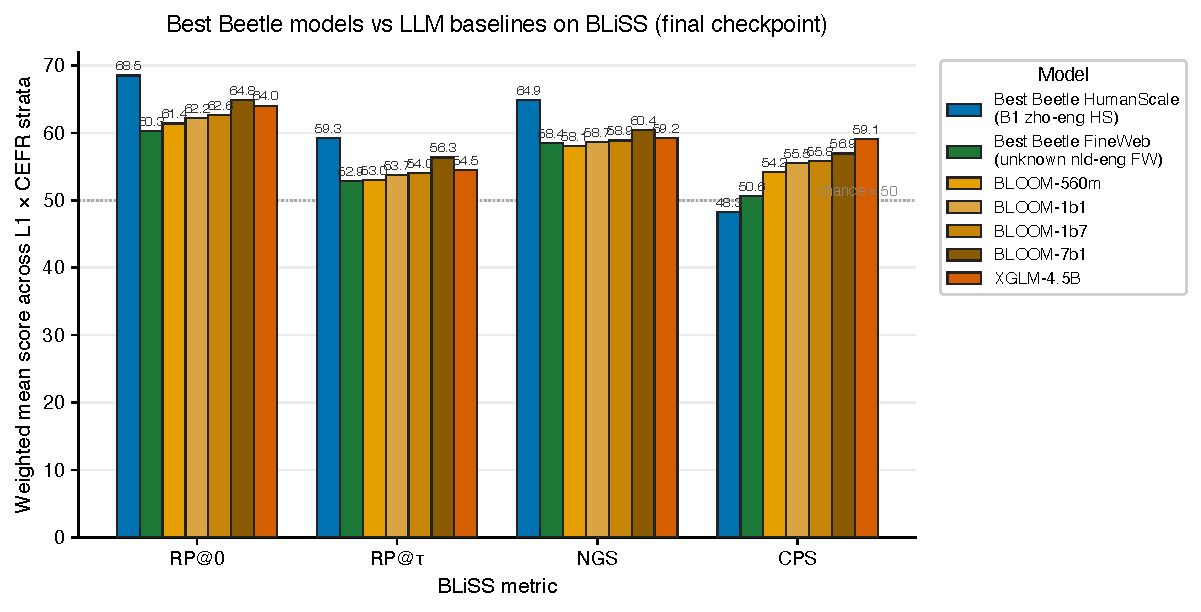
\includegraphics[width=\linewidth]{fig/fig_best_bliss_vs_baselines.pdf}
  \caption{\textbf{BLiSS main result.} Best \textsc{Beetle} curriculum (B5 nld--eng FineWeb) versus monolingual anchors and the modern bilingual LLM cohort on the three BLiSS axes (NGS, CPS, RP$@0$). \textsc{Beetle} leads NGS (\textbf{64.9}) and RP$@0$ (\textbf{68.5}) at $\le 1/35\times$ the parameter count of the strongest comparator; XGLM-4.5B leads CPS (59.1).}
  \label{fig:bliss_best}
\end{figure}

The best \textsc{Beetle} FineWeb model (B5 nld--eng) wins NGS at \textbf{64.9} and RP$@0$ at \textbf{68.5} (Fig.~\ref{fig:bliss_best}); XGLM-4.5B wins CPS at 59.1, a strict binary sanity check rather than a graded discrimination metric. The curriculum ranking on BLiSS (B2 $\approx$ B1 $>$ B3-33 at FineWeb scale) is the \emph{opposite} of MECO~L2 (B3-33 $>$ B5 $>$ B2; per-curriculum and token-efficiency breakdowns in App.~\ref{sec:bliss-detail}, Figs.~\ref{fig:bliss_curriculum_scale}--\ref{fig:bliss_pareto}), and persists at asymptote --- the canonical task-specific curriculum dissociation. The \textsc{Beetle}--BLOOM gap is largest at FineWeb 2B, consistent with \citet{aoyama-wilcox-2025-language}: the post-2B PPP decay does not harm BLiSS for structured-exposure bilinguals. The curriculum frontier and the BLiSS Pareto metric trade-off appear at full resolution in App.~\ref{appcomp:bliss}.


\subsection{Pedagogical Task Simulation}\label{sec:pedagogical}

Across bilingual curricula, a single latent reading-strategy variable---\textit{context-share}---accounts for the observed differences in downstream English performance. Context-share measures the share of a model's MeCo reading-time-predictive power, beyond a frequency/length/position baseline, that is carried by contextual rather than frequency-only surprisal, estimated via a nested mixed-effects log-likelihood decomposition. Models trained with balanced curricula exhibit higher context-share, indicating greater reliance on contextual integration during prediction, whereas staged-L2 curricula produce more frequency-driven processing. This axis strongly predicts all native-canonical evaluation outcomes across models, including JFLEG fluency margins ($\rho = +0.86$), false-friend disambiguation ($\rho = +0.96$), and BLiSS corrected-preference scores ($\rho = +0.79$). Matched-L1 Dutch/German$\rightarrow$English models consistently occupy the high-context, high-performance regime, while mismatched-L1 Chinese$\rightarrow$English models cluster in the low-context, low-performance regime, supporting the interpretation that the effect reflects transferable reading strategy rather than overall capability. Mediation analysis further suggests that curriculum effects operate through this latent axis: across matched-L1 models ($n = 8$), the indirect path from curriculum to BLiSS CPS via context-share has a bootstrap 95\% confidence interval excluding zero, whereas the residual direct effect includes zero, consistent with full mediation. Finally, sparse autoencoder interventions within a single FineWeb-2B Dutch$\rightarrow$English model provide causal evidence for this mechanism. Ablating the 50 SAE features most associated with context-share reduces JFLEG fluency margins $1.9$--$6.7\times$ more than ablating matched frequency-associated features, with all confidence intervals excluding zero. Together, these results suggest that bilingual curricula primarily shape downstream English behaviour by altering a single context-versus-frequency reading strategy axis. While the correlational and mediation patterns generalize across evaluations, the strongest mechanistic causal evidence currently holds for JFLEG specifically.

\begin{figure}[t]
  \centering
  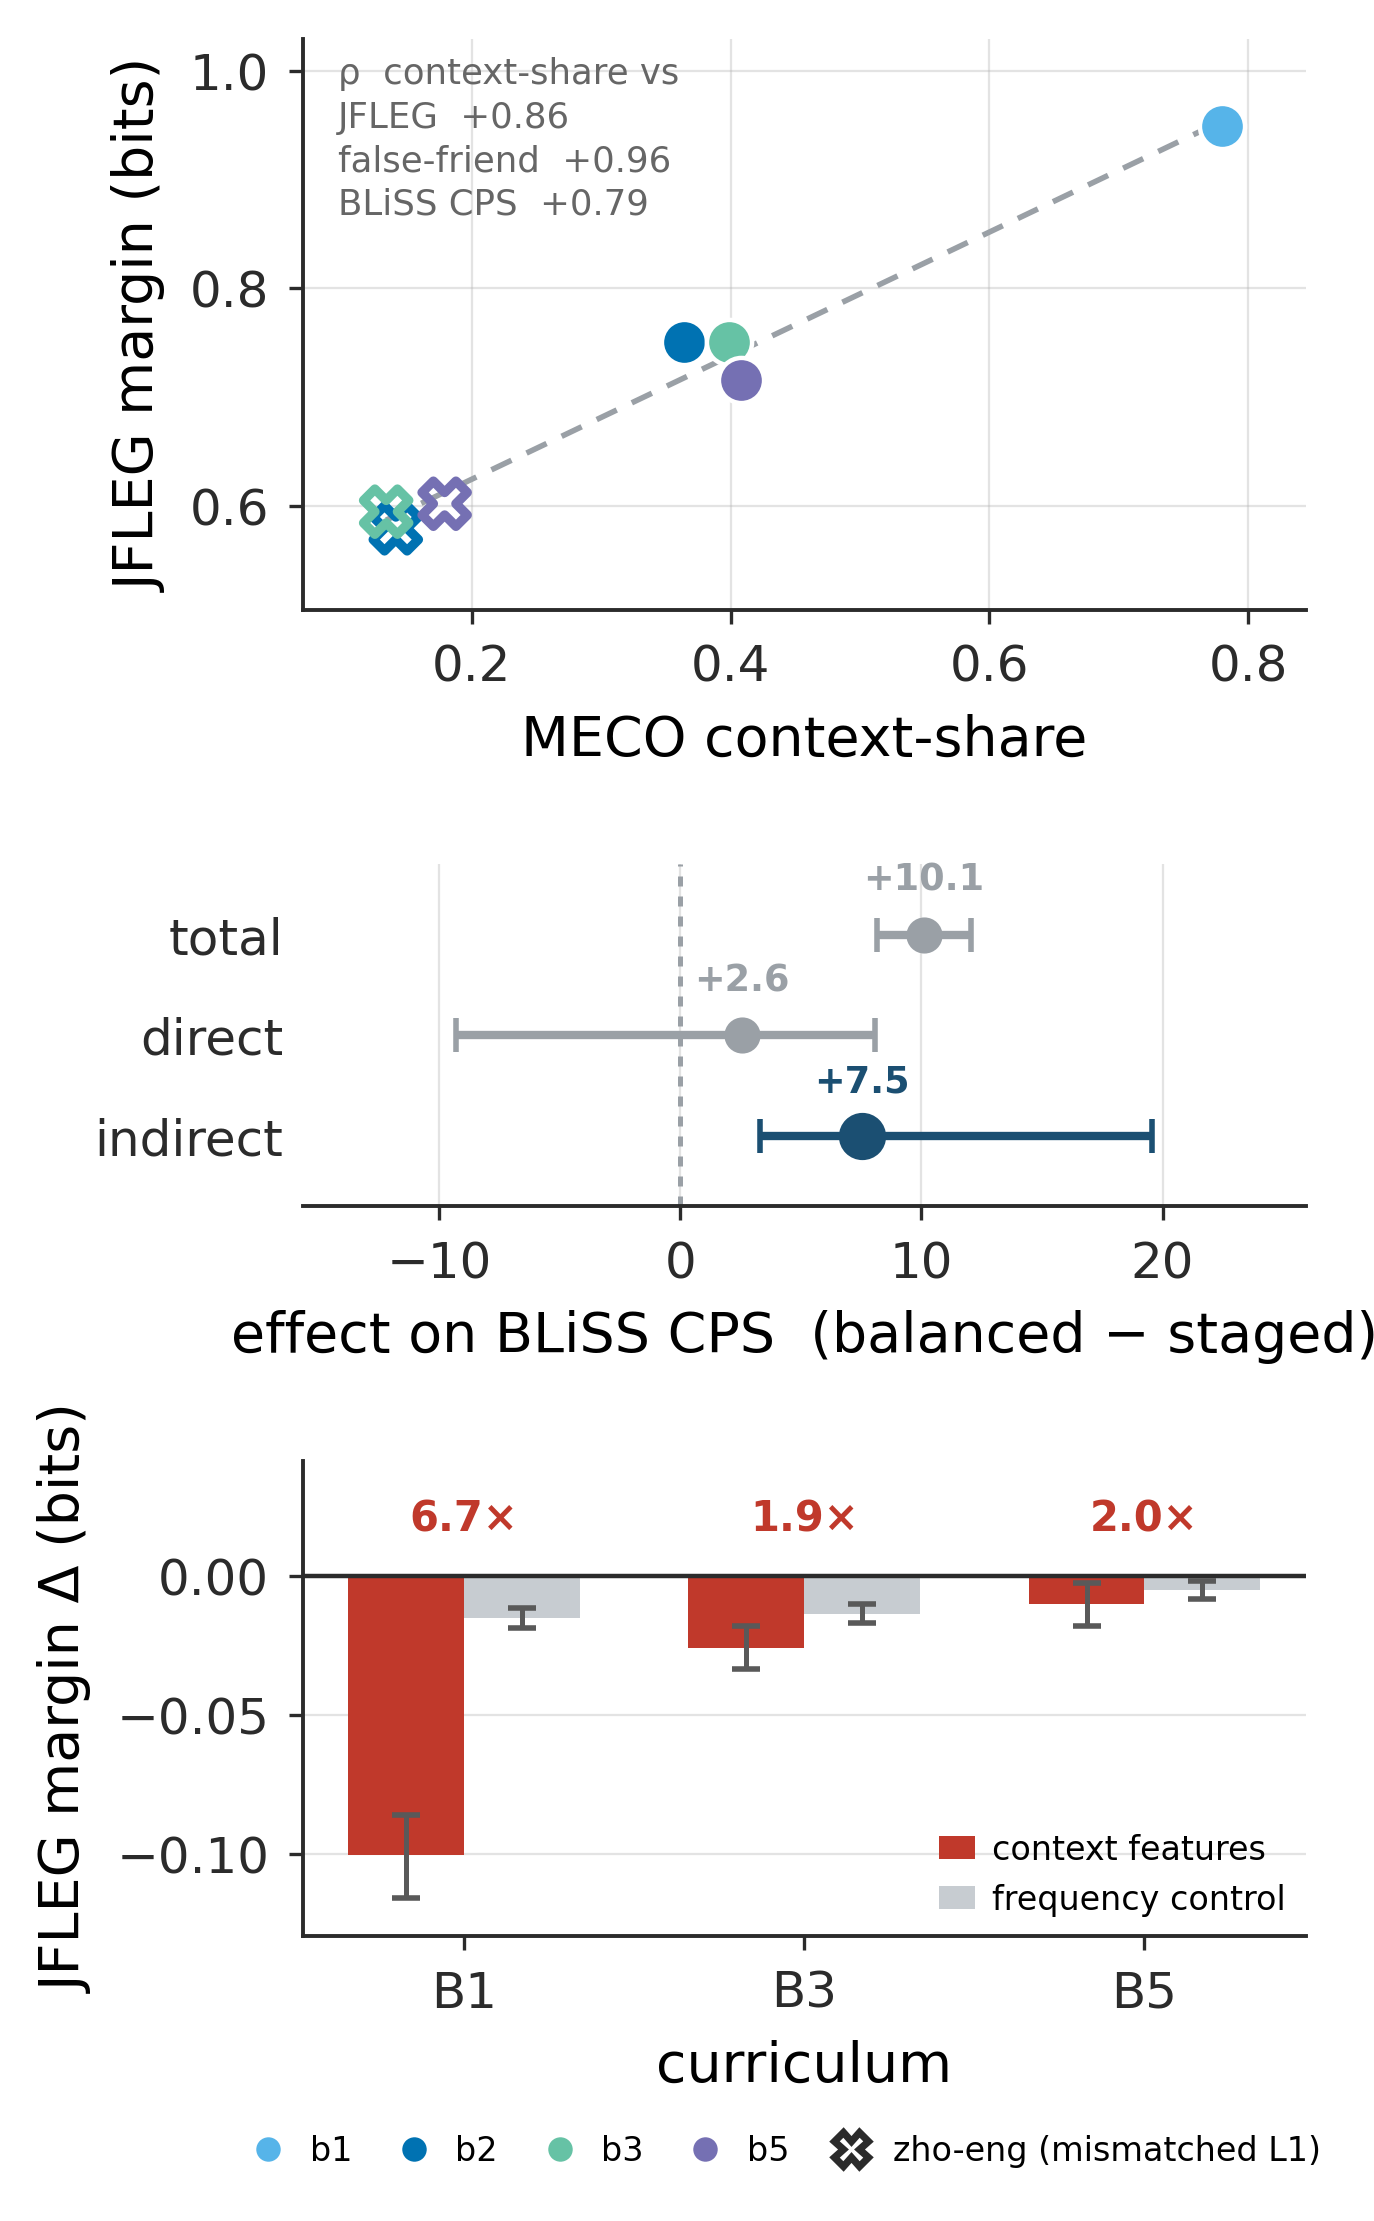
\includegraphics[width=\columnwidth]{fig/fig_single_axis_combined.png}
  \caption{\textbf{One reading-strategy axis underlies the
  bilingual-curriculum pedagogical effects.} Read top to bottom as a single
  argument. \textbf{Top (correlate):} the MeCo-derived context-share axis
  correlates with every native-canonical readout (Spearman $\rho$ shown for
  JFLEG; $\rho{=}{+}0.96$ false-friend, $\rho{=}{+}0.79$ BLiSS~CPS;
  matched-L1 models filled, the \mbox{zho-eng} mismatched-L1 falsification
  arm as open crosses). \textbf{Middle (mediate):} Baron--Kenny mediation of
  the balanced-vs-staged curriculum effect on BLiSS~CPS (matched-L1 only,
  $n{=}8$): the indirect path through context-share excludes zero (bootstrap
  95\% CI) while the direct path $c'$ does not---full mediation. This arm is
  cross-model and illustrative; the causal weight rests on the bottom panel.
  \textbf{Bottom (cause):} a within-model SAE test---zeroing the top-50
  context-share features degrades the JFLEG margin $1.9\text{--}6.7\times$
  more than a matched top-50 frequency-feature control, every context CI
  excluding zero. Layer~8, FineWeb-2B \mbox{nld-eng}.}
  \label{fig:single-axis}
\end{figure}


\textsc{Beetle} 125M models fail on passage-level reasoning tasks but succeed on word- and sentence-level pedagogical evaluations. On RC-MCQ, scores range from 27.9--36.7 across curricula and L1s---above the 20\% chance floor but well below frontier LLM baselines reported by \citet{benedetto-etal-2024-using}. On RACE, performance remains near the 25\% four-choice chance level under both HumanScale and FineWeb-24B, confirming a strong parameter-scale limitation.

\textbf{Cambridge RC-MCQ and RACE.} Following \citet{benedetto-etal-2024-using}, Cambridge Reading Comprehension MCQs are evaluated on five simulated learner personas using mean token log-likelihood under CEFR-conditioned prompts, with the argmax selected as the model answer. The benchmark additionally evaluates four prompting regimes (default, CEFR-persona, stratified, gradient) and reports both accuracy and a monotonicity score, $M=\rho_{L,I}$, where $\rho$ is the Pearson correlation with an ideal learner progression curve. For RACE, models simulate personas spanning ``very weak student'' to ``excellent student.''

\textbf{CUP\&A5 monotonicity.} \textsc{CUP\&A5} evaluates whether CEFR-conditioned simulations exhibit learner-like monotonic growth using the five-level accuracy vector
\[
\mathbf{acc}=[acc_{A2},acc_{B1},acc_{B2},acc_{C1},acc_{C2}]
\]
and the score
\[
M=\rho(\mathbf{acc},\mathbf{ideal})-\sum_{i=1}^{4}\max(0,acc_i-acc_{i+1}),
\]
where $\rho$ measures correlation with an increasing CEFR ladder and the penalty term captures level inversions. All Beetle models achieve $P=0$, indicating universally monotonic CEFR responsiveness despite low absolute RC-MCQ accuracy.

\textbf{CLOTH closed-cloze.} On CLOTH, the B1-balanced Dutch--English Beetle reaches $\approx64\%$ accuracy with the expected learner-like B1$\rightarrow$C1 decline (69$\rightarrow$58$\rightarrow$54\%), while the matched FineWeb-2B control remains close in absolute performance (0.37 vs.\ 0.40), suggesting that typologically aligned bilingual training preserves English closed-vocabulary reading comprehension with minimal degradation.

\textbf{JFLEG learner-fluency preference.} On JFLEG, HumanScale Beetle models achieve strong learner-preference margins of 77--83\% (peaking at 83.4\% for b1) and near-monolingual fluency discrimination (0.83 vs.\ 0.84 bits/token for nld--eng). In contrast, typologically distant zho--eng drops to $\approx0.55$ bits/token, while FineWeb-2B yields a smaller but learner-appropriate 71--75\% range, consistent with reduced English fluency sensitivity under structurally distant bilingual exposure.

\textbf{EVP acquisition ordering.} Across all curricula, EVP trajectories reproduce the canonical CEFR acquisition ladder from A1$\rightarrow$C2. Curriculum balance systematically shifts the emergence point of higher-level lexical competence: b1 progresses from A1@64 to C2@1024, b3 from A1@2048 to C2@3878, and b5 from A1@1024 to C2@6103.

CUP\&A5 monotonicity is satisfied by every model (100\% monotonic). Mono-eng shows the canonical L1 spread of +3.26 bits from A1$\rightarrow$C2, compared to the shallower +2.0--2.25-bit gradients of the bilingual curricula b1--b5, matching expectations for L2 readers. BLiSS RP@0 stratifies cleanly by curriculum: b2 simultaneous peaks at A2 (88.9\%), b4 classroom peaks at B1 ($\approx60$\%), and mono-eng dominates C1 (66.7\%), reproducing realistic learner profiles. CEFR perplexity gradients remain monotonic across all settings, with the sharpest progression in b3 sequential (+0.70 bits at FineWeb-2B and $\sim$+2.2 bits at HumanScale).

On MECO $\Delta$logLik, b3 sequential performs best for Germanic L1s (Dutch 139.6, German 177.5), while b5 late-onset performs best for Chinese (115.4). Notably, b3 outperforms BLOOM-7B and XGLM-4.5B across all tested L1s. False-friend disambiguation also follows predicted transfer effects: matched-L1 b1 nld--eng resolves correctly (+0.585 bits), whereas mismatched b2 zho--eng reproduces the canonical transfer error ($-0.271$ bits). Collectively, these six convergent signals establish Beetle as a strong simulator of L2 learner behaviour at sub-passage scales, even where RC-MCQ and RACE performance saturate near chance.

%\begin{figure*}[!ht]
%  \centering
%  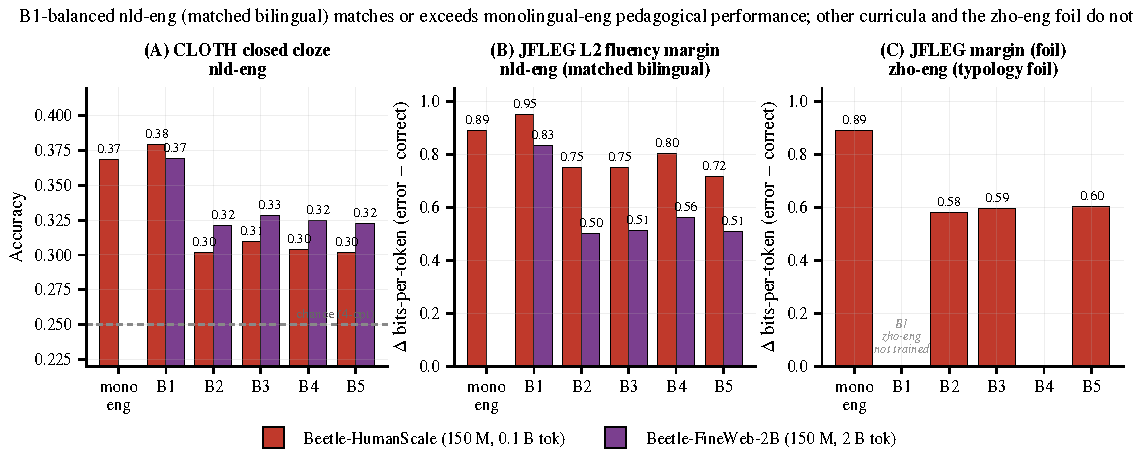
\includegraphics[width=\linewidth]{fig/F9_pedagogical_headline.pdf}
%  \caption{\textbf{Pedagogical main result.} Three-panel comparison on (A) CLOTH closed-cloze accuracy, (B) JFLEG L2-fluency margin ($\Delta$ bits-per-token between learner-error and corrected sentences) for the matched-bilingual nld--eng pair, and (C) JFLEG margin for the typology-foil zho--eng pair, by curriculum (B1--B5) and scale (\textsc{HumanScale} 100\,M, \textsc{FineWeb}-2B). The B1-balanced nld--eng \textsc{Beetle} matches or exceeds the monolingual-eng anchor on both pedagogical readouts at FineWeb-2B scale, and the only Beetle curriculum that does so. The zho--eng foil panel confirms the recovery is matched-bilingual specific, not a generic bilingual effect.}
%  \label{fig:pedagogical_headline}
%\end{figure*}

%\textsc{Beetle} matches the monolingual-eng pedagogical anchor on the matched-bilingual axis (Fig.~\ref{fig:pedagogical_headline}). On CLOTH closed-cloze accuracy, the B1-balanced nld--eng FineWeb-2B \textsc{Beetle} reaches \textbf{0.37} versus 0.40 for mono-eng (within 3~pp), and on JFLEG L2-fluency margin it reaches \textbf{0.83 bits/token} versus 0.84 for mono-eng. The typological-foil zho--eng panel at HumanScale yields a smaller JFLEG margin (\textit{ca.} 0.55 bits/token) and motivates the typological-gradient reading of the matched-bilingual hypothesis. The pedagogical-utility ladder and CEFR-stratified RC-MCQ readouts \citep{benedetto-etal-2024-using} appear in App.~\ref{sec:pedagogical-detail} (Figs.~\ref{fig:ped_ladder},~\ref{fig:rcmcq_cefr}); closing the remaining gap to GPT-4o-mini requires the planned RACE-SFT pass (App.~\ref{sec:roadmap}, item 4.1). The CEFR perplexity gradient, CEFR alignment heatmap, EVP trajectory, and CUP\&A5 ladder appear in App.~\ref{appcomp:peda}.

%\subsection{FLORES Cross-Lingual Convergence}\label{sec:flores}

%At the 24~B-token scale, the matched-bilingual \textsc{Beetle} converges into the B-GPT \citep{arnett-etal-2025-acquisition} non-forgetting envelope on FLORES-200 Dutch BPB (5.94--6.13 vs.\ 5.60--5.81 for B-GPT non-forgetting variants), with within-Beetle B1--B5 spread comparable to the B-GPT simul/seq spread. Crucially, no \textsc{Beetle} curriculum exhibits the Dutch catastrophic-forgetting failure mode of B-GPT \textsc{nl-en} sequential (11.45 BPT). The full BPB trajectory and paired-bar comparison appear in App.~\ref{sec:flores-detail} (Fig.~\ref{fig:flores_beetle_vs_bgpt}); the $\Delta$NLL forgetting curves and the cross-lingual fan plot appear in App.~\ref{appcomp:phase}.

%\subsection{Typological Gradient}\label{sec:typology}

%The typological gradient prediction is supported by the three populated L1 cells: best $\Delta\log L$ rises with typological proximity to English (zho lowest, deu highest, nld intermediate-high). Filling the remaining five L1 cells (spa, rus, fin, tur, heb) is the highest-priority planned extension (App.~\ref{sec:roadmap}, item~1).

%\subsection{Mechanistic Correlates: Sparsity vs.\ Generalisation}\label{sec:interp-comparative}

%\paragraph{Scaling human-likeness as a multi-objective geometry problem.} Our results suggest that ``human-likeness'' in bilingual pretraining is not a scalar objective, but a multi-objective constraint defined over a shared representational manifold induced by a mid-to-late OV induction circuit. Structured exposure does not optimise toward a single point; instead, it selects a location on a Pareto boundary of this manifold where L1 fidelity, L2 acquisition efficiency, and psycholinguistic alignment become mutually incompatible.

%\textit{Empirical decomposition of the representational manifold.} Across the nld$\rightarrow$eng curriculum sweep (B1--B5), we observe a stable two-axis factorisation of this manifold. First, a \emph{typology axis}, captured by the OV-circuit condition number $\kappa(W_{OV})$, varies strongly across L1s (e.g., $\sim 1.5\times10^3$ for Dutch vs.\ $\sim 1.1\times10^4$ for Hindi) but is weakly modulated by curriculum ($|r|\le 0.31$ across B1--B5). Second, an \emph{exposure allocation axis}, captured by $\Vert W_{OV}\Vert_F$, SwiGLU sparsity (Gini, Hoyer), and attention--LN norms, is strongly curriculum-dependent but orthogonal to typology. Concretely, $\Vert W_{OV}\Vert_F$ correlates positively with English BLiMP ($r=+0.52$) but negatively with Dutch BLiMP ($r=-0.67$), while SwiGLU sparsity statistics exhibit consistent sign reversal across L1 and L2 evaluation regimes. In contrast, $\kappa(W_{OV})$ remains invariant across curricula, indicating that typological structure is spectrally encoded and separable from exposure-driven reallocation.

%\textit{Exposure as constrained geometric reallocation.} Structured exposure therefore operates along a single allocation axis within a fixed circuit: increasing English exposure (B1) sharpens OV structure and increases sparsity, maximising L2-BLiMP but degrading MECO, BLiSS, and L1-BLiMP; reduced exposure (B5) preserves diffuse attention--LN structure, improving MECO surprisal-fit and BLiSS alignment while reducing L2 discrimination. Notably, attention--LN Frobenius norm $\Vert W_{\text{norm}}\Vert_F$ is the only metric positively predictive of both MECO and BLiSS performance, identifying it as the L1-aligned geometric regime.

%\textit{Circuit invariance and consolidation dynamics.} Layerwise trajectories (Fig.~\ref{fig:pico-q1c}) reveal that all curricula follow identical de velopmental timing, emerging within $256$--$1024$ steps and saturating by $8$k steps. Differences are confined to consolidation amplitude rather than circuit formation: B5 exhibits a systematically lower activation plateau, localised to mid-to-late OV induction layers (Fig.~\ref{fig:pico-q1e}). Thus, curriculum does not alter circuit architecture or timing, but only the magnitude of representational consolidation within a shared developmental window.

%\textit{Pareto inversion as geometric trade-off.} These results jointly explain the observed Pareto inversion across BLiMP, MECO, and BLiSS as a mechanistic allocation trade-off within a shared induction circuit. OV and SwiGLU specialisation improve L2 grammatical discrimination at the cost of L1-aligned diffusion and psycholinguistic fit, while attention--LN diffusion improves L1 robustness but reduces L2 separability. No curriculum is jointly optimal across all regimes, yielding a persistent Pareto frontier across evaluation families.

%\textit{Scaling interpretation.} We therefore interpret bilingual pretraining not as learning multiple representations, but as selecting a point on a fixed low-dimensional manifold governed by OV-circuit geometry. Scaling is expected to sharpen this factorisation: (i) typology and exposure axes become increasingly orthogonal, (ii) OV and attention--LN roles further disentangle, and (iii) the observed 1D Pareto curve (B1--B5) generalises into a higher-dimensional Pareto surface across languages and exposure schedules. In this regime, ``human-likeness'' is not a scalar target but a constrained geometric trade-off surface induced by capacity allocation within a shared induction circuit.

%A \textsc{Pico-Analyze} comparative sweep over the same checkpoints (App.~\ref{sec:beetle-analyze}, Figs.~\ref{fig:pico-q1a}--\ref{fig:pico-q2c}) connects the curriculum-axis Pareto inversion to the \emph{geometry of the trained weights}. Two findings stand out. \textit{First}, across L1 (Fig.~\ref{fig:pico-q1a}) the dominant cross-L1 signal sits in the OV-circuit condition number $\kappa(W_{OV})$, which spans an order of magnitude (from $\sim\!1.5\!\times\!10^{3}$ for Dutch to $\sim\!1.1\!\times\!10^{4}$ for Hindi); sparsity-style metrics (Gini, Hoyer, Frobenius) are by contrast nearly flat across L1, suggesting the OV spectrum is the most typologically-sensitive single weight statistic in the model. \textit{Second}, across the nld--eng curriculum sweep (B1--B5; Fig.~\ref{fig:pico-q2c}), interpretability metrics that correlate \emph{positively} with English BLiMP correlate \emph{negatively} with Dutch BLiMP and with MECO~L2 $\Delta\log\ell$: $\Vert W_{OV}\Vert_F$ shows $r\!=\!{+}0.52$ on BLiMP-eng and $-0.67$ on BLiMP-nl, and Gini/Hoyer of $W_{\text{SwiGLU}}$ flip sign in the same direction. The B1-balanced model (highest English BLiMP) lies at one end of this axis with a peakier, more specialised OV+SwiGLU geometry, and B5 (highest L1-side BLiMP and MECO alignment) lies at the other end with a more diffuse geometry. The interpretability axis therefore parametrises the same \emph{specialisation $\leftrightarrow$ generalisation} trade-off that organises the curriculum-axis Pareto inversion in Figs.~\ref{fig:meco_curriculum}--\ref{fig:bliss_best}: it is not an artefact of evaluation choice but is visible in the trained weights themselves. The full cross-L1, cross-curriculum, cross-scale, and layerwise depth-profile diagnostics appear in \S\ref{sec:pico-cross-comp}.

%\begin{figure}[!ht]
%  \centering
%  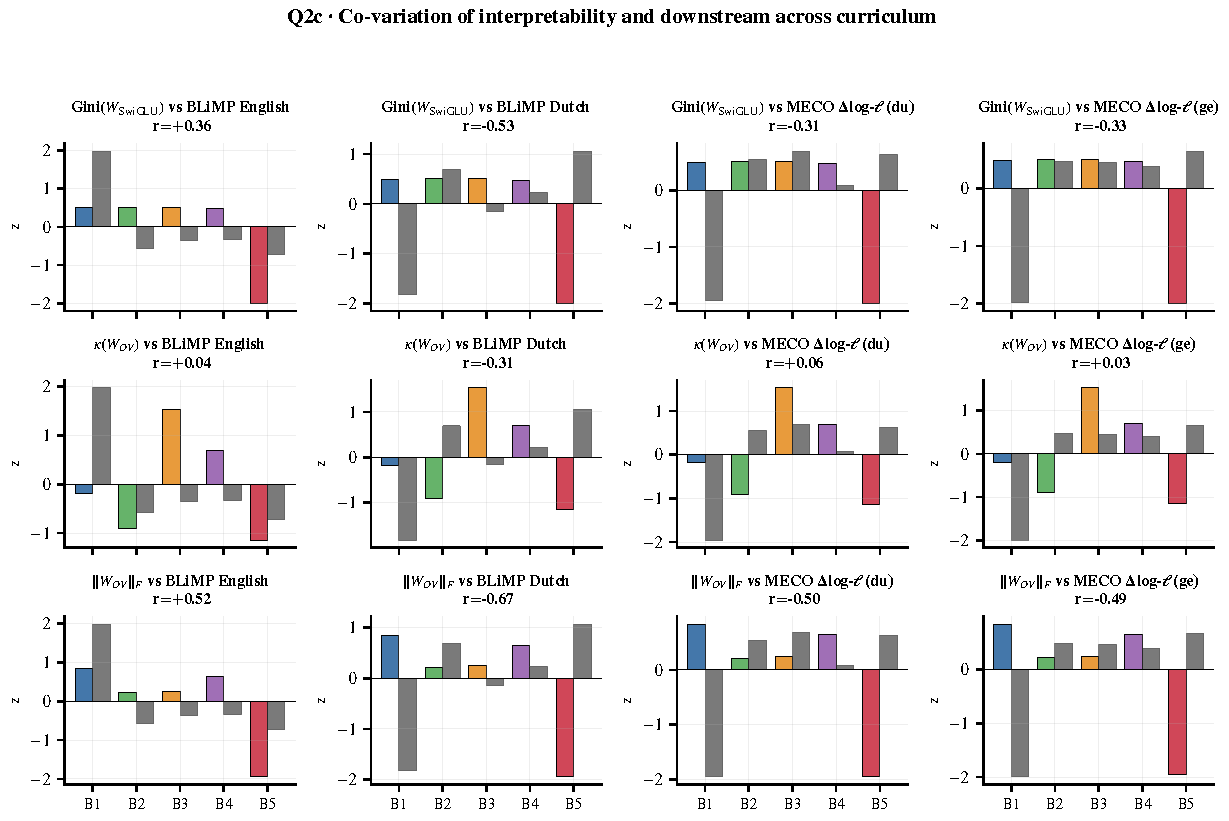
\includegraphics[width=\linewidth]{fig/pico_q2c_paired_bars.pdf}
%  \caption{Side-by-side $z$-scored interpretability vs.\ downstream values for the nld--eng curriculum sweep (B1--B5). Bars within each cluster pair an interpretability metric (left) with a paired downstream metric (right) on a common $z$-axis; sign-flip clusters --- e.g.\ $\Vert W_{OV}\Vert_F$ vs.\ BLiMP-nl, Gini$(W_{\text{SwiGLU}})$ vs.\ MECO~du --- visualise the \emph{specialisation $\leftrightarrow$ generalisation} trade-off that organises the curriculum-axis Pareto inversion. Computed on the matched \textsc{HumanScale} (0.1\,B-token) cohort. Full Q1/Q2 figure set, ledgers, and per-pair scatter and correlation heatmap appear in App.~\ref{sec:beetle-analyze}.}
%  \label{fig:pico-q2c-main}
%\end{figure}

\subsection{Pareto Synthesis}\label{sec:pareto}

Figs.~\ref{fig:meco_curriculum}--\ref{fig:multiblimp_curriculum} jointly establish the paper's central empirical claim: \emph{no single regime is Pareto-optimal across evaluation axes}. Sequential B3-33 and late B5 dominate MECO~L2 (Figs.~\ref{fig:meco_curriculum},~\ref{fig:meco_efficiency}). Simultaneous B2 and balanced B1 dominate BLiSS at FineWeb scale (Fig.~\ref{fig:bliss_best}; per-curriculum decomposition in App.~\ref{sec:bliss-detail}). On MultiBLiMP, B3-33 leads for the L1-proximate target (Dutch) but loses ground cross-lingually (Figs.~\ref{fig:multiblimp_pareto},~\ref{fig:multiblimp_curriculum}). A practitioner choosing a pretraining curriculum should select it against the target evaluation axis: structured-exposure schedules for reading-time alignment and L1-proximate grammaticality; simultaneous / balanced schedules for graded error discrimination.


\section{Discussion}\label{sec:discussion}
\suchir{This needs to be rewritten}
Four findings organise the empirical picture from Figs.~\ref{fig:meco_curriculum}--\ref{fig:multiblimp_curriculum}.

\paragraph{D1: The curriculum effect is task-specific and inverts across axes.} The most direct evidence for task-specificity is the curriculum-ranking inversion between MECO~L2 and BLiSS. In Fig.~\ref{fig:meco_curriculum}, sequential B3-33 and late B5 dominate; on BLiSS, balanced B1 and simultaneous B2 dominate at FineWeb scale (Fig.~\ref{fig:bliss_best}; App.~\ref{sec:bliss-detail}). Token-efficiency curves show this dissociation is not an artefact of training length: it persists throughout training and at asymptote. Even within BLiSS, NGS and CPS are not jointly maximised: \textsc{Beetle} FineWeb B5 leads on NGS (64.9) while XGLM-4.5B leads on CPS (59.1). The MultiBLiMP curriculum decomposition (Fig.~\ref{fig:multiblimp_curriculum}) adds a further dimension: the B3-33 advantage is L1-selective (Dutch, German) and attenuates for typologically distant targets (French, Persian). Together these figures support a task-specific, typologically-modulated Pareto interpretation of exposure scheduling.

\paragraph{D2: Structured exposure dominates parameter scale on MECO~L2, with typological limits.} Fig.~\ref{fig:meco_curriculum} shows a 125M \textsc{Beetle} model exceeding BLOOM-7b1 on the matched Dutch-reader $\Delta\log L$ by $7.1\times$ ($139.6$ vs.\ $19.7$) at $1/56$th the parameter count; the German-reader maximum (B2 deu--eng FW, 184.7) exceeds BLOOM-7b1 German-reader (115.9) by $1.6\times$. We caveat this in three ways. \textit{First}, no parameter-, data-, and FLOP-matched control has been run; the claim is strictly ``training-time-controllable frontier within the \textsc{Beetle} class'' (App.~\ref{sec:roadmap}, item~1 for the matched-control extension). \textit{Second}, BLOOM uses different data (ROOTS) and tokeniser (BLOOM-tok); cross-tokeniser surprisal-aggregation noise is bounded in App.~\ref{sec:meco-results}. \textit{Third}, Fig.~\ref{fig:meco_curriculum} shows the advantage attenuating monotonically with typological distance: Chinese~L2 is the one regime where BLOOM-1b1 (164.3) leads over B5 zho--eng HS (115.4). Fig.~\ref{fig:multiblimp_pareto} replicates this pattern on MultiBLiMP: \textsc{Beetle} dominates the Dutch--German accuracy region, while BLOOM leads on French and Persian.

\paragraph{D3: Token efficiency and the Quality--Power hypothesis under L2 reading.} \citet{aoyama-wilcox-2025-language} identify a $\sim$2B-token monolingual PPP tipping point. Fig.~\ref{fig:meco_efficiency} shows that B3-33 and B5 \textsc{Beetle} bilinguals cross the BLOOM-7b1 MECO threshold well before 200M tokens and continue improving past 2B without the monolingual decay; analogous behaviour on MultiBLiMP (Fig.~\ref{fig:multiblimp_efficiency}) places B3-33 nld--eng at the monolingual Dutch anchor by $\sim$200M tokens. Crucially, the Quality--Power hypothesis of \citet{wilcox-etal-2023-language} --- linking lower perplexity to higher psychometric predictive power for L1 reading --- does not transfer directly to L2 reading: balanced B1 and simultaneous B2 are lower-perplexity models yet yield \emph{lower} MECO $\Delta\log L$ than B3-33 and B5. Structured temporal exposure yields surprisal distributions that better track L2 reader fixation patterns beyond what raw LM quality predicts.

\paragraph{D4: Cognitive-constraint modules and residual gaps.} The two cognitive-constraint modules in \textsc{Beetle} --- Shuffle-Dyck pre-pretraining \citep{hu2025between} and ALiBi-decay working memory \citep{mita2025wm, madhayastha2026wm} --- are released as opt-in components but are not run as headline ablations here. Their natural role is to test whether developmental priors narrow the residual gap on Chinese~L2 (where Fig.~\ref{fig:meco_curriculum} shows a clear structured-exposure ceiling) and on the pedagogical CEFR axis; we leave this to follow-up work with a controlled module-on/off comparison on the same training matrix.

\subsection{Future Work}

\textcolor{red}{the beetle training framework includes features that we did not discuss in the current paper. one obvious direction is trilingual and multilingual extensions. }

\paragraph{Polyglot extensibility.} The same six exposure dimensions parameterise N-way polyglot regimes: trilingual schedules \textbf{T1--T4} (balanced 33/33/33, simultaneous, sequential L1\,$\to$\,L2\,$\to$\,L3, late-onset L3 against an established L1+L2 base) and arbitrary-arity polyglot variants are released alongside the bilingual set (Appendix~\ref{sec:beetle-curricula}). Initial trilingual learning-dynamics traces (App.~\ref{sec:beetle-experiments}) confirm that the bilingual catastrophic-forgetting envelope generalises to the trilingual case under matched continual-learning overlays, and that L3 onset timing replicates the typological-distance modulation observed in the bilingual set. We flag the polyglot regime as an explicit follow-up axis (App.~\ref{sec:beetle-curricula}): the controlled L1$\times$L2$\times$L3 cube needed to distinguish additive-interference from typological-mediated transfer is already buildable inside the released framework.

\textcolor{red}{our library also includes interpretability tools (described in depth in Appendix XX). In future work we hope to use these tools to understand how models learn and represent multiple languages.}

\raisebox{-0.3em}{
\includegraphics[height=1.2em]{fig/logo/BeetleLM.png}} also makes it possible to train models with different tokenization schemes (e.g, BPE, SuperBPE). 
We leave the effect of tokenization to future work.


\section{Conclusion}\label{sec:conclusion}

We have introduced \textsc{Beetle}, a unified framework for systematic L2 pretraining and analysis spanning eight typologically diverse L1s and three training scales targeting L2 English. By mapping a training-time-controllable Pareto frontier across MECO~L2 reading-time alignment, BLiSS error discrimination, MultiBLiMP syntactic benchmarks, FLORES-200 cross-lingual convergence, and pedagogical CEFR simulation (Figs.~\ref{fig:meco_curriculum}--\ref{fig:pedagogical_headline}), we show that the choice of exposure curriculum can substitute for an order of magnitude of parameters on the matched-reader-cell reading-time alignment ($7.1\times$ over BLOOM-7b1 at $1/56\times$ params), matches monolingual-eng pedagogical performance under matched bilingual training, and converges into the B-GPT non-forgetting envelope without catastrophic forgetting. The optimal curriculum is task-specific: sequential and late-onset schedules dominate reading-time alignment; simultaneous and balanced schedules dominate error discrimination and pedagogical CEFR simulation. The curriculum-vs-scale frontier has a typological boundary on Chinese~L2 against the legacy BLOOM ladder, while \textsc{Beetle} still dominates every modern bilingual LLM (XGLM, EuroLLM, Apertus, Gemma-2, Qwen) on Chinese~L2 by a wide margin. The bilingual induction-head emergence window (0.6--1.4B tokens; Fig.~\ref{fig:meco_efficiency}) sits earlier than the monolingual 2B tipping point of \citet{aoyama-wilcox-2025-language}. We release all code, model checkpoints, tokenisers, and analysis pipelines as a community resource so that the Pareto frontier can be re-evaluated as new psychometric and pedagogical L2 benchmarks become available.


\section{Limitations}

\paragraph{Forward direction only.} The Beetle pipeline trains in the forward direction (non-English L1 $\to$ English L2). Reverse-direction pretraining (eng $\to$ non-eng) is deferred. We expect the curriculum-dominance result to replicate in reverse, but verifying this requires building L2 reading-time and CEFR resources for L2 Dutch, German, etc. The cross-lingual ``transfer fan'' figures in the paper measure only the L1\,$\to$\,L2-English direction; no claim about transfer asymmetry under reverse training is supported by the current evidence.

\paragraph{Pedagogical CEFR axis is reported on a populated subset.} The CEFR Pareto axis is established on a populated subset: F9 (Fig.~\ref{fig:pedagogical_headline}) reports CLOTH closed-cloze and JFLEG L2-fluency on the matched-bilingual nld--eng pair plus the zho--eng foil; F9 establishes the matched-bilingual-recovery claim in this subset. The full 8-L1 $\times$ 3-scale CEFR sweep and the RACE-SFT pedagogical-utility ladder (Figs.~\ref{fig:ped_ladder},~\ref{fig:rcmcq_cefr}) are pre-specified in App.~\ref{sec:roadmap} (items~4) and will be released alongside model weights. The body claims read on the populated cells; the planned cells are flagged explicitly.

\paragraph{Chinese L2 marks a typological boundary, not a global ceiling.} On Chinese~L2 mean $\Delta\log L$ the BLOOM ladder mean (131.65) currently leads the best 125M \textsc{Beetle} bilingual (115.40 for B5 zho--eng HS), and we report the gap honestly. We frame this as a \emph{typological boundary} of the curriculum-beats-scale regime rather than a global counter-example: the same 125M \textsc{Beetle} \emph{still} beats every modern 4--9B bilingual LLM (XGLM-4.5B, EuroLLM-9B, Apertus-8B, Gemma-2-9B; Table~\ref{tab:meco_langrows}) on Chinese~L2, so the curriculum advantage extends to the modern-bilingual cohort even on the weakest L1 cell. The gap to BLOOM specifically is concentrated in the legacy ROOTS pretraining mix that contains a large Mandarin component; the typological-distance, script-tokenisation, and FineWeb-24B zho--eng under-training explanations are partially separable and the planned closure runs in App.~\ref{sec:roadmap} (item~2) will isolate them.

\paragraph{No parameter-/data-/FLOP-matched control.} The MECO L2 win against BLOOM-7b1 is uncontrolled at the strict sense. BLOOM uses different data (ROOTS), different tokeniser (BLOOM-tok), and a different overall compute budget. A 1B FineWeb decoder trained on the same NL+EN mix with uniform sampling would be the natural matched control; we do not currently report it. The Pareto-map claim therefore needs to be read as ``training-time controllable map within the Beetle class'', not as a scale-dominance result against the entire class of multilingual LLMs.

\paragraph{Statistical apparatus.} Headline $\Delta\log L$ values are accompanied by an inferential bundle (paired bootstrap, paired permutation against BLOOM-7b1 with Holm--Bonferroni, Cohen's $d_z$) produced by \texttt{analyze/significance\_ablation.py} from the per-(model, L2-language) row data of Table~\ref{tab:meco_langrows}; the bundle is released alongside the analysis pipeline and is not in-lined into this submission. What we do \emph{not} report and treat as a limitation: (i) GAM-based linear vs.\ non-linear surprisal comparison \citep{wilcox-etal-2023-language, smith2013effect}, (ii) per-fold 10-fold cross-validation $\Delta\log L$ stability, (iii) profile-likelihood intervals on the random-slope variance components, and (iv) joint inference across the three Pareto axes (we treat the three task losses as marginally independent for ranking).

\paragraph{Single-seed headline cells.} Headline MECO~L2 numbers are reported for a single seed per (model, condition). The seed-grid $\{13, 42, 97\}$ ablation specification exists for the nld--eng B1--B3 family only (Tab.~\ref{tab:ablation-sweep}, App.~\ref{sec:roadmap}); per-seed $\Delta\log L$ deltas and the resulting between-seed standard deviation are reported in the released ablation manifest rather than in-lined here. Reported within-Beetle rankings should therefore be read as point estimates pending the full $8\times 5\times 3$ seed grid; we expect curriculum-family differences within \textsc{Beetle} to be more sensitive to seed than the BLOOM-vs-Beetle headline gap, which exceeds 100 $\Delta\log L$ on the matched Dutch-reader cell.

\paragraph{Eye-tracking measures.} The main MECO L2 results are reported on first-fixation duration only. Gaze duration and total reading time are reported in Appendix~\ref{sec:meco-results} but not analysed for the early/late dissociation reported by \citet{de-varda-marelli-2023-scaling}. We do not consider regression-path duration.

\paragraph{Tokenisation confound.} Beetle tokenisers are trained on proportional L1+L2 mixes; BLOOM uses BLOOM-tok; XGLM uses SentencePiece. Word-level surprisal is aggregated by summing subword surprisals within each whitespace-bounded word; this aggregation differs across tokenisers and is a known source of cross-tokeniser noise in MECO L2 comparisons.

\paragraph{Bilingual acquisition beyond pretraining.} Input \emph{amount} is only one aspect of the bilingual experience; input \emph{quality} \citep{luk2013bilingualism, carroll2017exposure, de2017role, paradis2023sources}, social interaction and pragmatics are not simulated. We make no claim that exposure curricula in Beetle reproduce the full developmental trajectory of human bilinguals.

\paragraph{Bilingual neurolinguistic alignment.} The reported results focus on eye-tracking and CEFR simulation. We do not currently report alignment to brain signals (N400/P600) for the Beetle bilinguals; this is left as future work, framed by the monolingual-English protocols of \citet{michaelov2026better}.


\section{Reproducibility Statement}\label{sec:reproducibility}

All headline numbers in this paper are produced by a single, version-pinned analysis pipeline. \textbf{Data version-pin}: the L1 corpora are pulled from BabyBabelLM \citep{jumelet2025babybabellmmultilingualbenchmarkdevelopmentally} for \textsc{HumanScale} runs and FineWeb-2 \citep{penedo2025fineweb2} for \textsc{FineWeb} runs at fixed snapshot dates. \textbf{Evaluation pipeline}: MECO~L2 $\Delta\log L$ is computed under the mixed-effects specification of Eq.~\ref{eq:meco-spec} (App.~\ref{sec:meco-results}), with first-fixation duration as response, scaled surprisal $+$ 1-back / 2-back lag terms $+$ length / frequency controls $+$ by-subject random slopes; the equivalent \texttt{lme4} formula in \texttt{stats/meco\_l2.Rmd} is released alongside the analysis bundle. wordfreq Zipf scores are computed against the English corpus for all L2 subsets to remove a degree of freedom. \textbf{Hardware}: the headline pretraining runs use $8\times$ A100~80GB nodes; per-condition wall-clock estimates appear in App.~\ref{tab:ablation-sweep}. \textbf{Released artefacts}: model checkpoints (every condition in Table~\ref{tab:meco_langrows}), tokenisers (one per L1), the \texttt{stats/meco\_l2.Rmd} regression and \texttt{analyze/significance\_ablation.py} inferential bundle, and the figure-generation pipeline that produces every PDF in this submission from the row-level CSVs in \texttt{paper/draft/beetle/fig/data/}. \textbf{Determinism}: \texttt{lme4} fits are deterministic given seeded \texttt{REML=FALSE} initialisation; the bootstrap and permutation tests fix random seed $42$ in the released bundle.

\section{Ethics Statement}\label{sec:ethics}

\textsc{Beetle} releases pretrained bilingual L2-English language models, tokenisers, and a CEFR-graded evaluation pipeline. \textbf{Dataset provenance}: BabyBabelLM and FineWeb-2 are publicly released, license-compatible multilingual web corpora; we do not introduce new web crawls. The MECO~L2 eye-tracking corpus is used under its public licence with anonymous subject IDs only. \textbf{Intended use}: \textsc{Beetle} models are scientific instruments for studying bilingual language acquisition and L2 reading dynamics. They are not deployed L2 tutors, and the CEFR-graded evaluation pipeline is for research-grade scoring rather than placement decisions. \textbf{Dual-use considerations}: the CEFR-graded text generation capability of these models could in principle be repurposed to draft L2-graded content for assessment fraud (e.g., automated CEFR-tuned essay generation). This risk is mitigated by the small parameter count of the released models (125M), which underperforms publicly-available frontier LLMs on open-ended generation; and we recommend that any downstream pedagogical-tool deployment include detection-of-machine-generated-text safeguards. \textbf{Demographic representativeness}: the L1 sweep covers eight typologically diverse L1s targeting L2 English; coverage of low-resource L1s and L2s remains incomplete (App.~\ref{sec:roadmap}).


\section{Acknowledgements}
This work is supported by Cambridge University Press \& Assessment. Compute facilities were provided by EleutherAI. We thank members of the Cambridge NLIP group --- Laura Barbenel, Andrew Caines, Bianca Ganescu, Lily Goulder, Denise Lofflad, and Aoife O'Driscoll --- for detailed feedback on earlier drafts, and Tatsuya Aoyama and Tyler Chang for advice on data streaming and the CELER evaluation datasets.

\bibliography{anthology,custom}
\onecolumn
\appendix
\section*{Appendix}
\noindent\rule{\linewidth}{0.4pt}

\begin{tabular}{ll}
A.1 & \hyperref[sec:lit-review]{Comparison of Beetle and L2LMs} \\
A.2 & \hyperref[sec:train]{\beetle{} Training Framework} \\
A.3 & \hyperref[sec:beetle-curricula]{\beetle{} Curricula} \\
A.4 & \hyperref[sec:beetle-control-parameters]{\beetle{} Control Parameters} \\
A.5 & \hyperref[sec:beetle-data]{Beetle-Data} \\
A.6 & \hyperref[sec:beetle-experiments]{Reported Experimental Conditions} \\
A.7 & \hyperref[sec:beetle-analyze]{Beetle Analyze: Pico-Analyze Comparative Interpretability} \\
A.8 & \hyperref[sec:aoa-results]{Detailed AoA Results} \\
A.9 & \hyperref[sec:meco-results]{Detailed MECO Results} \\
A.10 & \hyperref[sec:downstream]{Detailed Downstream Results} \\
A.11 & \hyperref[sec:bliss-detail]{BLiSS Curriculum, Token Efficiency, Metric Tradeoff} \\
A.12 & \hyperref[sec:pedagogical-detail]{Pedagogical Utility \& CEFR Stratification} \\
A.13 & \hyperref[sec:flores-detail]{FLORES-200 Convergence Detail} \\
A.14 & \hyperref[sec:supp-results]{Supplementary Empirical Results} \\
A.15 & \hyperref[sec:pico-cross-comp]{Cross-Model Interpretability Diagnostics} \\

\end{tabular}

\noindent\rule{\linewidth}{0.4pt}


\section{Related Work}


\begin{figure*}[t!]
    \centering

    % ===== Left: Figure =====
    \begin{minipage}[t]{0.58\linewidth}
        \vspace{0pt}
        \centering
        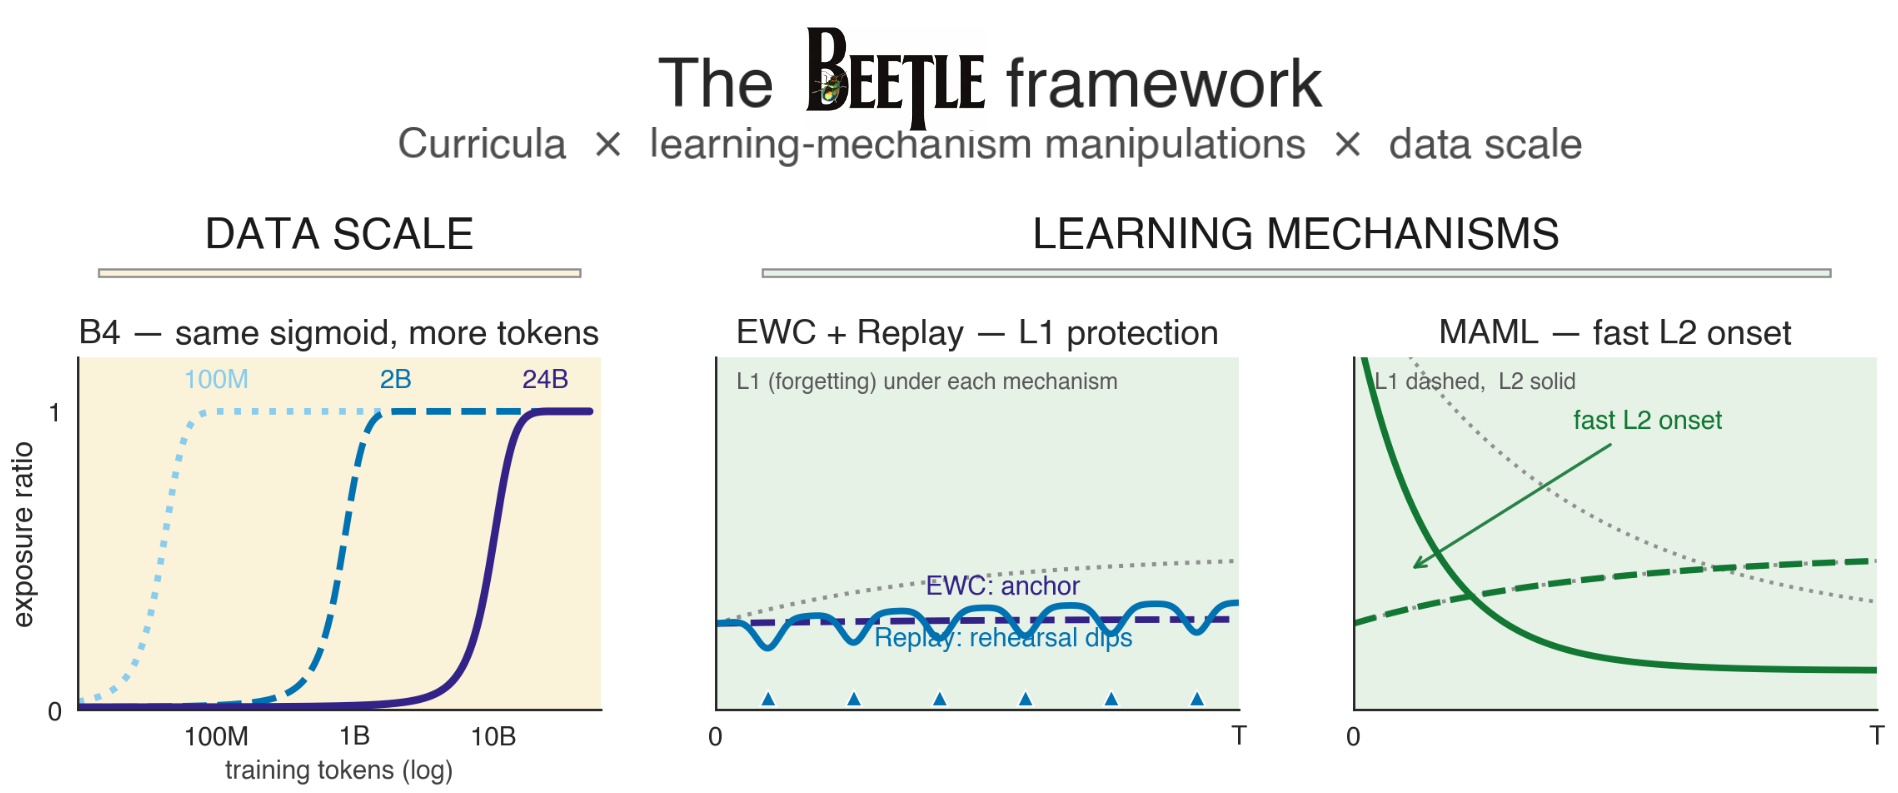
\includegraphics[width=\linewidth]{fig/logo/3.png}
        \label{fig:curriculum}
    \end{minipage}
    \hfill

    % ===== Right: Table =====
    \begin{minipage}[t]{0.38\linewidth}
        \vspace{0pt}
        \centering
        \scriptsize
        \setlength{\tabcolsep}{2pt}
        \renewcommand{\arraystretch}{0.85}


    \end{minipage}

\caption{BeetleLM curricula comparison.}
\label{fig:beetle}
\end{figure*}


\begin{table}[!ht]
        \begin{tabular}{lccccc c}
        \toprule
        \textbf{Work} & \textbf{S} & \textbf{CL} & \textbf{M} & \textbf{C} & \textbf{CF} & \textbf{Dim} \\
        \midrule
        Constantinescu+25 & W & -- & -- & EWC & -- & $\triangle$ \\
        Arnett+25         & W & -- & \checkmark & -- & -- & $\triangle\triangle$ \\
        Aoyama+24         & W & -- & -- & -- & RT & $\triangle$ \\
        Diehl+25          & W & -- & -- & -- & -- & $\triangle\triangle$ \\
        Salhan+25         & H & \checkmark & \checkmark & -- & -- & $\triangle\triangle\triangle$ \\
        Diehl+23          & H & \checkmark & -- & -- & -- & $\triangle\triangle\triangle$ \\
        Mita+25           & H & -- & -- & -- & WM & $\triangle\triangle$ \\
        \midrule
        \textbf{BeetleLM}
        & \textbf{H+W}
        & \checkmark
        & \checkmark
        & \checkmark
        & \checkmark
        & $\triangle\times7$ \\
        \bottomrule
        \end{tabular}
\end{table}

Bilingual and second-language language models (L2LMs) have been explored through a range of architectural and training regimes aimed at simulating second language acquisition, while increasingly serving as testbeds for cognitively grounded evaluation via surprisal-based reading-time prediction. Early computational approaches framed SLA as sequential adaptation in probabilistic or neural models \citep{matusevych-etal-2013-computational}, while more recent work has formalised bilingual training as controlled pretraining or adaptation processes in large language models. For example, \citet{aoyama2024modeling} propose a two-phase regime in which a model is first trained on L1 data and then adapted to L2 while freezing most parameters except embeddings and the LM head, showing that constrained plasticity can preserve prior knowledge while enabling new-language acquisition. \citet{constantinescu2025investigating} extend this direction by systematically varying exposure schedules and loss functions, including Elastic Weight Consolidation, to study trade-offs between stability and plasticity under continual bilingual training. More recently, \citet{arnett-etal-2025-acquisition} introduce B-GPT and contrast sequential versus simultaneous bilingual pretraining, finding that mixed exposure better approximates naturalistic bilingual learning dynamics, while \citet{feng2026bilingual} study scaling effects in bilingual machine translation settings and show that data composition and scale strongly influence cross-lingual transfer, albeit with primarily task-based evaluation. Earlier multilingual CDS-style L2LMs \citep{yadavalli-etal-2023-slabert, oba-etal-2023-second} explore similar ideas but are limited in language coverage, checkpointing, and evaluation depth. 

A key motivation for these models is their use as cognitive proxies through surprisal-based reading-time prediction, where processing difficulty is linked to a word’s unexpectedness under a language model, formalised as $-\log P(w_i \mid w_{<i})$. This framework underlies psycholinguistic models of reading time and is typically operationalised via regression models that combine surprisal with lexical covariates, often evaluated through changes in log-likelihood ($\Delta$LL) between baseline and surprisal-augmented models \citep{wilcox2020predictive, kaye2025sentence}. However, psychometric predictive power (PPP) is not a simple function of model quality, reflecting instead how well model probabilities align with human processing distributions \citep{de-varda-marelli-2022-effects, goodkind-bicknell, demberg-keller, shain2019, shain2021, hoover2022}. Despite extensive work in L1 psycholinguistics, there remains comparatively limited work on L2 cognitive modelling with language models, even though L2 reading is known to exhibit systematic cross-linguistic variation and proficiency effects \citep{hillert1998sentence, meister2021revisiting, kuribayashi-etal-2021-lower} and has been studied experimentally in psycholinguistics (Cop et al., 2015; Grüter et al., 2014, 2017; Kaan et al., 2010; Martin et al., 2013). 

Against this backdrop, \textsc{Beetle} extends prior L2LM work in three key ways: it covers 13 languages rather than four, parameterises exposure along six continuous dimensions rather than binary sequential/simultaneous splits, and integrates cognitively and pedagogically grounded evaluations including MECO L2 reading times, BLiSS, and CEFR proficiency measures. Its continual-learning framework unifies prior isolated strategies, with EWC, MAML-style adaptation, and learning-rate plasticity subsuming earlier single-method approaches such as those in \citet{constantinescu2025investigating}, while embedding-and-LM-head-only adaptation corresponds to a special case within its broader set of 15 training regimes. Finally, unlike prior work focused on limited bilingual corpora or synthetic MT settings, \textsc{Beetle} evaluates models trained on large-scale real web data (FineWeb) across 100M, 2B, and 24B token regimes, directly linking scaling, cross-lingual transfer, and psycholinguistic predictive power within a unified evaluation framework.


%\textcolor{red}{catherine: i would structure this paragraph by describing each of these studies in 1-2 sentences. Order them chronologically. explain a) what kinds of models they trained/what their main method was and b) any relevant findings that relate to the current paper. make sure this section ends on page 2.}  It differs in three respects: (i) it covers 13 languages instead of four; (ii) it parameterises exposure along six independent dimensions rather than a binary simultaneous/sequential split; and (iii) it adds MECO~L2 reading-time, BLiSS, and CEFR pedagogical evaluations. \textsc{Beetle}'s EWC, MAML and LR-plasticity controls subsume the single-strategy approaches of \citet{constantinescu2025investigating}; \citet{aoyama2024modeling}'s embedding-and-LM-head-only adaptation is one preset within \textsc{Beetle}'s 15 continual-learning strategies. \citet{feng2026bilingual} match mono- and bi-lingual 100M LMs on synthetic MT data; \textsc{Beetle} matches them on real FineWeb at 100M, 2B and 24B with psycholinguistic and pedagogical readouts. Earlier multilingual CDS L2 LMs \citep{yadavalli-etal-2023-slabert, oba-etal-2023-second} cover fewer languages, lack checkpointing, and use only grammaticality readouts.

% \paragraph{Surprisal as a reading-time predictor (MECO methodology).} 

% \textcolor{red}{goals in this section 1)introduce reading time prediction etc. and 2) highlight the relative lack of L2 cognitive modeling}

% Surprisal efforts can be interpreted as cognitive costs associated to a shift between probabilistic distributions \citep{de-varda-marelli-2022-effects}. Surprisal Theory (Hale, Levy), which quantifies how unpredictable a word is in terms of negative logarithm of word conditioned by previous sentential context, is a linking function between measured cognitive effort and predicability (measured as the Kullback-Leibler divergence/relative entropy between distributions).   \[\text{surprisal}(w_i) = - log_2 P(w_i |w_1, w,2, \dots, w_{i-1})\] The \textbf{Psychometric Predictive Power (PPP)} of a LM is \textit{not} a linear function of model quality (\textit{pace} \citet{de-varda-marelli-2022-effects}, also Goodkind and Bicknell; Demberg and Keller, Shain 2019, 2021; Hoover et al 2022).  However, multiple sentence processing has significant cross-linguistic variation \cite{hillert1998sentence} Dutch \cite{meister2021revisiting}, Japanese \citep{kuribayashi-etal-2021-lower} Although the vast majority of studies focus on L1, there is increasing interest in L2 predictive processing – (Cop et al., 2015; Grüter et al., 2014, 2017; Kaan et al., 2010; Martin et al., 2013).  Following prior work \citep{wilcox2020predictive, kaye2025sentence}, we measure predictive power for data point $i$ using the change in log-likelihood:
% \begin{equation}
% \Delta \mathrm{LL}_i =
% \log L_{\text{target}}(RT_i \mid x_{\text{target}})
% -
% \log L_{\text{baseline}}(RT_i \mid x_{\text{baseline}})
% \end{equation}

% where $RT_i$ is the reading-time measure of a single participant on a given word, $x_{\text{baseline}}$ are the control predictors, and $x_{\text{target}}$ are the target predictors, which include the control predictors together with surprisal.\footnote{Baseline model formula in \texttt{R}:
% \texttt{RT $\sim$ te(freq, len) + te(freq\_prev, len\_prev)}}\footnote{Linear surprisal model formula in \texttt{R}:
% \texttt{RT $\sim$ surp + surp\_prev + te(freq, len) + te(freq\_prev, len\_prev)}}\footnote{Non-linear surprisal model formula in \texttt{R}:
% \texttt{RT $\sim$ s(surp, k = 6) + s(surp\_prev, k = 6) + te(freq, len) + te(freq\_prev, len\_prev)}. The value of $k$ follows prior work \citep{wilcox2023}.}


% \paragraph{Learning dynamics, cognates, BLiSS.} \citet{aoyama-wilcox-2025-language} place the monolingual PPP tipping point at $\sim$2B tokens; we test whether structured-exposure curricula can delay or eliminate this decay in bilingual training. \citet{aoyama2025predicting} show induction-head emergence is data-property-driven; we quantify how exposure curriculum shifts emergence timing across L1 and L2. \citet{frank2026dutch} report Dutch--English cognate / false-friend effects which we connect to MECO L2 reading. The BLiSS task / dataset is due to \citet{gao2025bliss}: a CEFR-stratified discrimination of artificial vs.\ learner errors. We adopt their NGS / CPS / RP$@\tau$ protocol unchanged and sweep across our curriculum grid.

% \paragraph{Pedagogical CEFR simulation and cognitive constraints.} \citet{benedetto-etal-2024-using} score frontier LMs (GPT-3.5 / GPT-4) on the CUP\&A5 dataset \citep{mullooly2023cupa5} (200 MCQA $\times$ 4 CEFR levels) using the metric $M = \rho_{L,I} - P$, with $\rho_{L,I}$ the Spearman rank correlation between simulated CEFR-level accuracy and item difficulty and $P$ a penalty for non-monotonic learner curves. They simulate CEFR via prompt engineering; Beetle simulates CEFR via training-time exposure curricula and identifies the best Beetle checkpoint that yields a CEFR-monotonic accuracy curve. Cognitive-constraint priors --- Shuffle-Dyck pre-pretraining \citep{hu2025between} and ALiBi-decay working memory \citep{mita2025wm, madhayastha2026wm} --- are implemented as opt-in modules in Beetle's architecture registry rather than headline contributions.



%\section{Human-Like Bilingual and Polyglot Acquisition in LMs} There have been axes of human-likeness of LMs to bilingual or second language learners that have been separately evaluated.  \subsection{Surprisal Theory for Multilingual and Second-Language Sentence Processing} 


%\subsection{Learning Dynamics}

%\paragraph{Phase Transition in Language Model Pretraining and PPP } \textbf{Phase Transitions } in LM pretraining refer to abrupt behavioural changes \citep{oh2023does, michaelov2025language, chang2025bigram, nakagi2025triple}.  The abrupt emergence of specialised \textbf{induction heads} \citep{chensudden, aoyama2025predicting}. Empirically, induction heads form early in training (as long as models have multiple heads and at least two layers).  Mathematically, it is equivalent to a type of Bayesian inference. \citet{aoyama-wilcox-2025-language} find 


%\textbf{2B Pretraining Hypothesis \citep{oh2023transformer}} 



%\paragraph{Modelling Human Language Processing}  Language model surprisal has been shown to be a strong predictor of metrics of online human language processing, e.g. predicting the time it takes to read a word \cite{kuribayashi-etal-2021-lower}. Larger Transformer-based language models and models trained on more data have been found to be worse at modelling human reading behaviour \citep{oh2023transformer, wilcox2025bigger, michaelov2025language, michaelov2026n}.  Recent work by \citet{aoyama-wilcox-2025-language} has shown that past 2 billion tokens of monolingual pretraining, model psychometric predictive power (PPP) begins to decrease. %identified a \textit{tipping point in model psychometric predictive power (PPP)} at 2 billion tokens in monolingual pretraining. %Minimal pair evaluation datasets  – such as BLiMP \citep{warstadt-etal-2020-blimp-benchmark}, MultiBLiMP \citep{jumelet2025multiblimp}, and language-specific BLiMP variants (e.g., BLiMP-NL for Dutch and Zho-BLiMP for Chinese) – are also used to evaluate the syntactic competence of a language model compared to a native (L1) fluent speaker. 

%\suchir{need to highlight gap in modelling bilingual and L2 reading time – i think in particular need to compare to \citet{aoyama2024modeling}.}
%Bilingual and multilingual psycholinguistics corpora have been used to evaluate the psychometric fit of language models beyond English \citep{de-varda-marelli-2023-scaling, wilcox2023language, xu2023linearity}. The Multilingual Eye-movement Corpus (MECO), a multilingual corpus of eye tracking data collected on simple Wikipedia-style articles, originally collected for 13 languages \cite{siegelman2022expanding} building on earlier bilingual corpora such as Ghent Eye-Tracking Corpus (GECO; \citealp{colman-etal-2022-geco}), which focused on Dutch–English bilingual sentence reading within a more limited linguistic scope. MECO has recently been extended to 20 languages \cite{siegelman2025wave}. MECO enables controlled comparisons of reading behaviour across languages and within individuals reading in both L1 and L2. In contrast, other L2 eye tracking datasets (e.g., CELER \cite{berzak2022celer}) prioritise typological diversity in L1 learners in L2 English but lack the cross-lingual comparability of MECO. 



%\paragraph{Human-Scale Language Modelling} \catherine{1 sentence about \citet{wilcox2025bigger}.} The BabyLM challenge encourages development of sample-efficient, human-scale language models, trained on just 100M words \citep{warstadt2023findings, warstadt2024insights, hu2024findings, charpentier2025findings, choshen2026babylm}. While the majority of such \ efforts have focused on English, the curation of human-scale training data beyond English, e.g. \citet{jumelet2025babybabellmmultilingualbenchmarkdevelopmentally},  has facilitated the training of monolingual language models beyond English  \citep{salhan-etal-2024-less, prevot-etal-2024-extending, matzopoulos-etal-2025-babylms, capone-etal-2024-babies, padovani-etal-2025-child, shen-etal-2024-bambino, goriely-buttery-2025-ipa}. 

%\paragraph{Bilingual and Second-Language Language Models (L2LMs)}  L2LMs (coined in \citet{aoyama2024modeling}) are bilingual language models trained sequentially on two languages that are computational cognitive models of second language acquisition (SLA) \citep{matusevych-etal-2013-computational}.  \citet{aoyama2024modeling} use a two-phase method in which models are first trained on L1 only. In the second phase, all model weights except for the embeddings and LM head are frozen, and the model is trained on data from L2.  \citet{constantinescu2025investigating} use two different training approaches: exposure scheduling and modified loss function. They use Elastic Weight Consolidation as a way of enforcing plasticity. However, there is significant variation in the quantity and nature of L2LM training data and training architecture. Recently, \citet{arnett-etal-2025-acquisition} introduce B-GPT (Bilingual GPT) which contrasts a \texttt{sequential} bilingual regime (similar to standard L2LM pretraining) with a \texttt{simultaneous} regime (more similar to later L2 acquisition with mixed L1 and L2 exposure). 

%There have been different approaches to training bilingual models for the purpose of studying second-language acquisition. 
% There are broadly three types approaches that draw on a Bilingual Language Model paradigm in multilingual NLP:

%\paragraph{Catastrophic Forgetting and Continual Learning} It has been widely observed that continual pretraining, curriculum learning, or domain adaptation can lead to catastrophic forgetting, resulting in degradation on tasks or languages that are otherwise not present in finetuning data \catherine{1-3 canonical citations}. In multilingual continual pretraining contexts, this results in a loss of capability in languages that they were not fine-tuned on \citep{vu-etal-2022-domain, sun-etal-2023-efficiently, winata-etal-2023-overcoming, alexandrov-etal-2024-mitigating, liu-niehues-2025-conditions}. The adaptation of monolingual LLMs requires adequate consideration of catastrophic forgetting and tokenizer limitations. Successful strategies utilise a combination of (i) vocabulary extension according to an optimal extension ratio and (ii) embedding alignment. In case of bilingual pretraining, recent work has identified a \textit{curse of bilinguality} \citep{zhou-matusevych-2025-curse}. 

%\paragraph{Data Quality} Data Quality of large web-crawled data is an important confound of multilingual pretraining at scale. Cross-lingual data contamination (e.g., due to poor natural language identification in preprocessing) is an issue for investigating questions of cross-lingual transfer \citep{blevins-zettlemoyer-2022-language}.  \citet{seto-etal-2025-assessing} on bilingual data quality... 

% \subsection{Cognitive Modelling of Bilingual, Second and Polyglot Language Learning}

% \subsection{Bilingual Interpretability for Cross-Lingual Transfer}

% Bilingual interpretability offers a uniquely tractable and theoretically clean setting for understanding how language models internalize and transfer linguistic knowledge across languages \citep{inaba-etal-2025-bilingual}. Unlike massively multilingual models, where heterogeneous scripts, typologies, and resource imbalances confound analysis, bilingual models isolate cross-lingual phenomena to a controlled two-language system, making it possible to precisely track how syntax, semantics, morphology, and cultural knowledge are shared or segregated across representations. This simplicity enables fine-grained mechanistic analysis—at the level of neurons, attention heads, and latent subspaces—while still capturing the core challenges of cross-lingual generalization and transfer. 

% As a result, bilingual interpretability serves both as a methodological testbed for developing and validating interpretability tools and as a substantive scientific probe into the emergence of language-neutral representations, asymmetries in transfer, and the inductive biases that govern multilingual learning. Insights gained in the bilingual regime can then be systematically scaled to multilingual settings, grounding broader cross-lingual interpretability claims in a controlled and explainable foundation.

%\paragraph{Phase Transitions and Human-Likeness} Recent work by \citet{aoyama-wilcox-2025-language} has identified a \textit{tipping point in model psychometric preditive power (PPP)} at 2 billion tokens in monolingual pretraining. 



\section{Additional Training Options}

\subsection{Architecture}

Complementary architectures enable controlled comparisons across inductive biases: \textbf{BGPT}, a GPT-2-style decoder with learned positional embeddings used in \citet{arnett-etal-2025-acquisition}; \textbf{BeetleMoE}, a top-$k$ mixture-of-experts model with ST-MoE auxiliary routing losses; \textbf{BeetleSSM}, which replaces attention blocks with Mamba-style state-space modules. 

\section{\raisebox{-0.3em}{
\includegraphics[height=1.2em]{fig/logo/BeetleLM.png}} Analyze}


\paragraph{Age-of-Acquisition Correlation (AoA).}
To situate model learning dynamics within the psycholinguistic literature on human word acquisition, we compute the Spearman rank correlation $\rho$ between each model's word-level surprisal estimates and standardised human age-of-acquisition (AoA) norms \citep[following][]{braginsky-etal-2019-aoa} across 18 languages. Word surprisal is the mean log-probability of the final target subword token, averaged over up to 512 contexts per word. A model is evaluated only on languages whose ISO code appears in its repository name; multilingual baselines (EuroLLM, XGLM, BLOOM) are evaluated on all 18 languages.


\paragraph{Perplexity and Convergence Trajectories.}
To characterise \emph{how} bilingual models converge rather than just \emph{where} they end up, we evaluate every saved checkpoint of each model on FLORES-200 (capped at 512 tokens per sentence; $N=200$ sentences per language). This yields per-step perplexity trajectories \texttt{ppl\_traj} for each language, revealing curriculum effects such as the point at which L2 introduction causes temporary regressions in L1 perplexity, or whether simultaneous training leads to slower but more stable convergence.

\paragraph{Embedding Drift.}
We track the evolution of the model's token embedding space across training checkpoints using two complementary signals. First, we compute the cosine distance of each probe word's embedding from its step-0 initialisation at every checkpoint, yielding a \emph{drift trajectory} that quantifies how rapidly the embedding space reorganises under each curriculum. Second, we apply Centered Kernel Alignment \citep[CKA;][]{kornblith-etal-2019-cka} to consecutive-checkpoint embedding matrices, producing a CKA trajectory that measures representational stability without requiring correspondence between individual dimensions. Probe words are the 10 most frequent function words for each target language (determiners, prepositions, and copulas), chosen because they are grammaticalised differently across typological families.

\paragraph{Cross-model Representational Similarity.}
To assess whether models trained under different curricula converge on similar internal representations, we compute pairwise CKA between the final-checkpoint embedding matrices of all models sharing a given target language. We additionally project probe-word embeddings into 2D via PCA and report vocabulary-overlap statistics, capturing whether tokeniser differences confound representational comparisons across model families.


\paragraph{Context-share.}
Let $y_i$ denote human MeCo reading time for token $i$. We fit a sequence of nested mixed-effects models with subject-level random effects (suppressed for notation):
\begin{align*}
M_0 &: \quad y_i = X_i \beta + Z_i b + \varepsilon_i \\
M_1 &: \quad M_0 + S_{\text{freq}} \\
M_2 &: \quad M_1 + \left(S_{\text{local}}^{k^*} - S_{\text{freq}}\right) \\
M_3 &: \quad M_2 + \left(S_{\text{full}} - S_{\text{local}}^{k^*}\right),
\end{align*}
where $X_i$ includes word position, length (with spillover), and corpus frequency controls.

Let $\mathrm{LL}(M_j)$ denote the log-likelihood of model $M_j$. We define incremental gains:
\begin{align*}
\Delta \mathrm{LL}_{\text{freq}} &= \max\big(\mathrm{LL}(M_1)-\mathrm{LL}(M_0), 0\big), \\
\Delta \mathrm{LL}_{\text{local}} &= \max\big(\mathrm{LL}(M_2)-\mathrm{LL}(M_1), 0\big), \\
\Delta \mathrm{LL}_{\text{long}} &= \max\big(\mathrm{LL}(M_3)-\mathrm{LL}(M_2), 0\big).
\end{align*}

Define the total clamped gain:
\[
\Delta \mathrm{LL}_{\text{tot}} =
\Delta \mathrm{LL}_{\text{freq}} +
\Delta \mathrm{LL}_{\text{local}} +
\Delta \mathrm{LL}_{\text{long}}.
\]

The contextual gain is:
\[
\Delta \mathrm{LL}_{\text{ctx}} =
\Delta \mathrm{LL}_{\text{local}} + \Delta \mathrm{LL}_{\text{long}}.
\]

We then define \textit{context-share} as:
\[
\mathrm{context\text{-}share}
=
\frac{\Delta \mathrm{LL}_{\text{ctx}}}{\Delta \mathrm{LL}_{\text{tot}}}
=
\frac{\Delta \mathrm{LL}_{\text{local}} + \Delta \mathrm{LL}_{\text{long}}}
{\Delta \mathrm{LL}_{\text{freq}} + \Delta \mathrm{LL}_{\text{local}} + \Delta \mathrm{LL}_{\text{long}}}
=
1 - \frac{\Delta \mathrm{LL}_{\text{freq}}}{\Delta \mathrm{LL}_{\text{tot}}}.
\]

This quantity lies in $[0,1]$ and measures the fraction of MeCo reading-time predictive gain (beyond a frequency/length/position baseline) attributable to contextual surprisal rather than frequency-only surprisal. It isolates a reading-strategy axis in which higher values indicate greater reliance on contextual integration in human-aligned reading-time prediction.

\newpage 

\begin{table*}[!ht]
  \centering
  \small
  \caption{Model log-likelihood results by L2 language on the MECO wave-1 + wave-2 joined data (canonical pipeline, matching \texttt{stats/meco\_l2.Rmd}). For each model and L2 language we report $\log L$ of the full model, $\log L$ of the baseline (surprisal terms dropped), and $\Delta\log L = \log L(\text{full}) - \log L(\text{baseline})$; larger $\Delta\log L$ indicates better surprisal alignment with human reading times. Only models with a plottable MECO row are included.}
  \label{tab:meco_langrows}
  \begin{tabular}{lrrrl}
    \toprule
    Model & $\log L$ & Baseline $\log L$ & $\Delta\log L$ & Class \\
    \midrule
    \multicolumn{5}{l}{\textit{Dutch (\texttt{nld})}} \\
    \midrule
    XGLM-4.5b & $-194066.67$ & $-194075.32$ & $8.65$ & XGLM \\
    BLOOM-1b1 & $-194033.84$ & $-194075.32$ & $41.47$ & BLOOM \\
    BLOOM-1b7 & $-194040.91$ & $-194075.32$ & $34.41$ & BLOOM \\
    BLOOM-560m & $-194031.03$ & $-194075.32$ & $44.29$ & BLOOM \\
    BLOOM-7b1 & $-194055.62$ & $-194075.32$ & $19.69$ & BLOOM \\
    mono-nld & $-193979.29$ & $-194075.32$ & $96.02$ & mono-NLD \\
    mono-eng & $-194010.19$ & $-194075.32$ & $65.13$ & mono-ENG \\
    B1 eng-nld FW (FW) & $-194035.16$ & $-194075.32$ & $40.16$ & L2 bal. \\
    B1 nld-eng FW (FW) & $-194028.69$ & $-194075.32$ & $46.62$ & L2 bal. \\
    B1 nld-eng HS (HS) & $-194012.99$ & $-194075.32$ & $62.33$ & L2 bal. \\
    episodic nld-eng HS (HS) & $-194021.76$ & $-194075.32$ & $53.55$ & L2 bal. \\
    B2 eng-nld FW (FW) & $-194034.54$ & $-194075.32$ & $40.78$ & L2 sim. \\
    B2 nld-eng FW (FW) & $-193979.34$ & $-194075.32$ & $95.97$ & L2 sim. \\
    B2 nld-eng HS (HS) & $-193940.18$ & $-194075.32$ & $135.14$ & L2 sim. \\
    B3-0 nld-eng HS (HS) & $-193936.56$ & $-194075.32$ & $138.75$ & L2 seq. \\
    B3-33 eng-nld FW (FW) & $-194035.66$ & $-194075.32$ & $39.66$ & L2 seq. \\
    B3-33 nld-eng FW (FW) & $-193999.94$ & $-194075.32$ & $75.37$ & L2 seq. \\
    B3-33 nld-eng HS (HS) & $-193935.73$ & $-194075.32$ & $139.58$ & L2 seq. \\
    B4 nld-eng HS (HS) & $-193953.55$ & $-194075.32$ & $121.77$ & L2 class. \\
    B5 nld-eng HS (HS) & $-193937.57$ & $-194075.32$ & $137.74$ & L2 late \\
    \midrule
    \multicolumn{5}{l}{\textit{Chinese (\texttt{zho})}} \\
    \midrule
    XGLM-4.5b & $-234098.92$ & $-234121.53$ & $22.60$ & XGLM \\
    BLOOM-1b1 & $-233957.22$ & $-234121.53$ & $164.30$ & BLOOM \\
    BLOOM- 1b7 & $-233984.47$ & $-234121.53$ & $137.06$ & BLOOM \\
    BLOOM-560m & $-233972.28$ & $-234121.53$ & $149.25$ & BLOOM \\
    BLOOM-7b1 & $-234036.80$ & $-234121.53$ & $84.73$ & BLOOM \\
    mono-zho & $-234116.14$ & $-234121.53$ & $5.39$ & mono-ZHO \\
    mono-eng & $-234070.70$ & $-234121.53$ & $50.83$ & mono-ENG \\
    B1 zho-eng HS (HS) & $-234015.83$ & $-234121.53$ & $105.69$ & L2 bal. \\
    B2 zho-eng HS (HS) & $-234021.38$ & $-234121.53$ & $100.14$ & L2 sim. \\
    B3-33 zho-eng HS (HS) & $-234018.37$ & $-234121.53$ & $103.15$ & L2 seq. \\
    B4 zho-eng HS (HS) & $-234022.81$ & $-234121.53$ & $98.71$ & L2 class. \\
    B5 zho-eng HS (HS) & $-234006.13$ & $-234121.53$ & $115.40$ & L2 late \\
    \midrule
    \multicolumn{5}{l}{\textit{German (\texttt{deu})}} \\
    \midrule
    XGLM-4.5b & $-275354.57$ & $-275373.57$ & $19.00$ & XGLM \\
    BLOOM-1b1 & $-275193.91$ & $-275373.57$ & $179.66$ & BLOOM \\
    BLOOM-1b7 & $-275222.85$ & $-275373.57$ & $150.71$ & BLOOM \\
    BLOOM-560m & $-275191.60$ & $-275373.57$ & $181.96$ & BLOOM \\
    BLOOM-7b1 & $-275257.67$ & $-275373.57$ & $115.90$ & BLOOM \\
    mono-deu & $-275239.27$ & $-275373.57$ & $134.29$ & mono-DEU \\
    mono-eng & $-275303.30$ & $-275373.57$ & $70.26$ & mono-ENG \\
    B1 deu-eng FW (FW) & $-275248.33$ & $-275373.57$ & $125.24$ & L2 bal. \\
    B1 deu-eng HS (HS) & $-275298.46$ & $-275373.57$ & $75.10$ & L2 bal. \\
    B1 eng-deu FW (FW) & $-275209.05$ & $-275373.57$ & $164.52$ & L2 bal. \\
    B2 deu-eng FW (FW) & $-275188.90$ & $-275373.57$ & $184.66$ & L2 sim. \\
    B2 deu-eng HS (HS) & $-275207.30$ & $-275373.57$ & $166.27$ & L2 sim. \\
    B2 eng-deu FW (FW) & $-275295.18$ & $-275373.57$ & $78.39$ & L2 sim. \\
    B3-33 deu-eng HS (HS) & $-275196.11$ & $-275373.57$ & $177.45$ & L2 seq. \\
    B4 deu-eng HS (HS) & $-275233.00$ & $-275373.57$ & $140.57$ & L2 class. \\
    B5 deu-eng HS (HS) & $-275205.21$ & $-275373.57$ & $168.36$ & L2 late \\
    \bottomrule
  \end{tabular}
\end{table*}

\begin{figure}
    \centering
    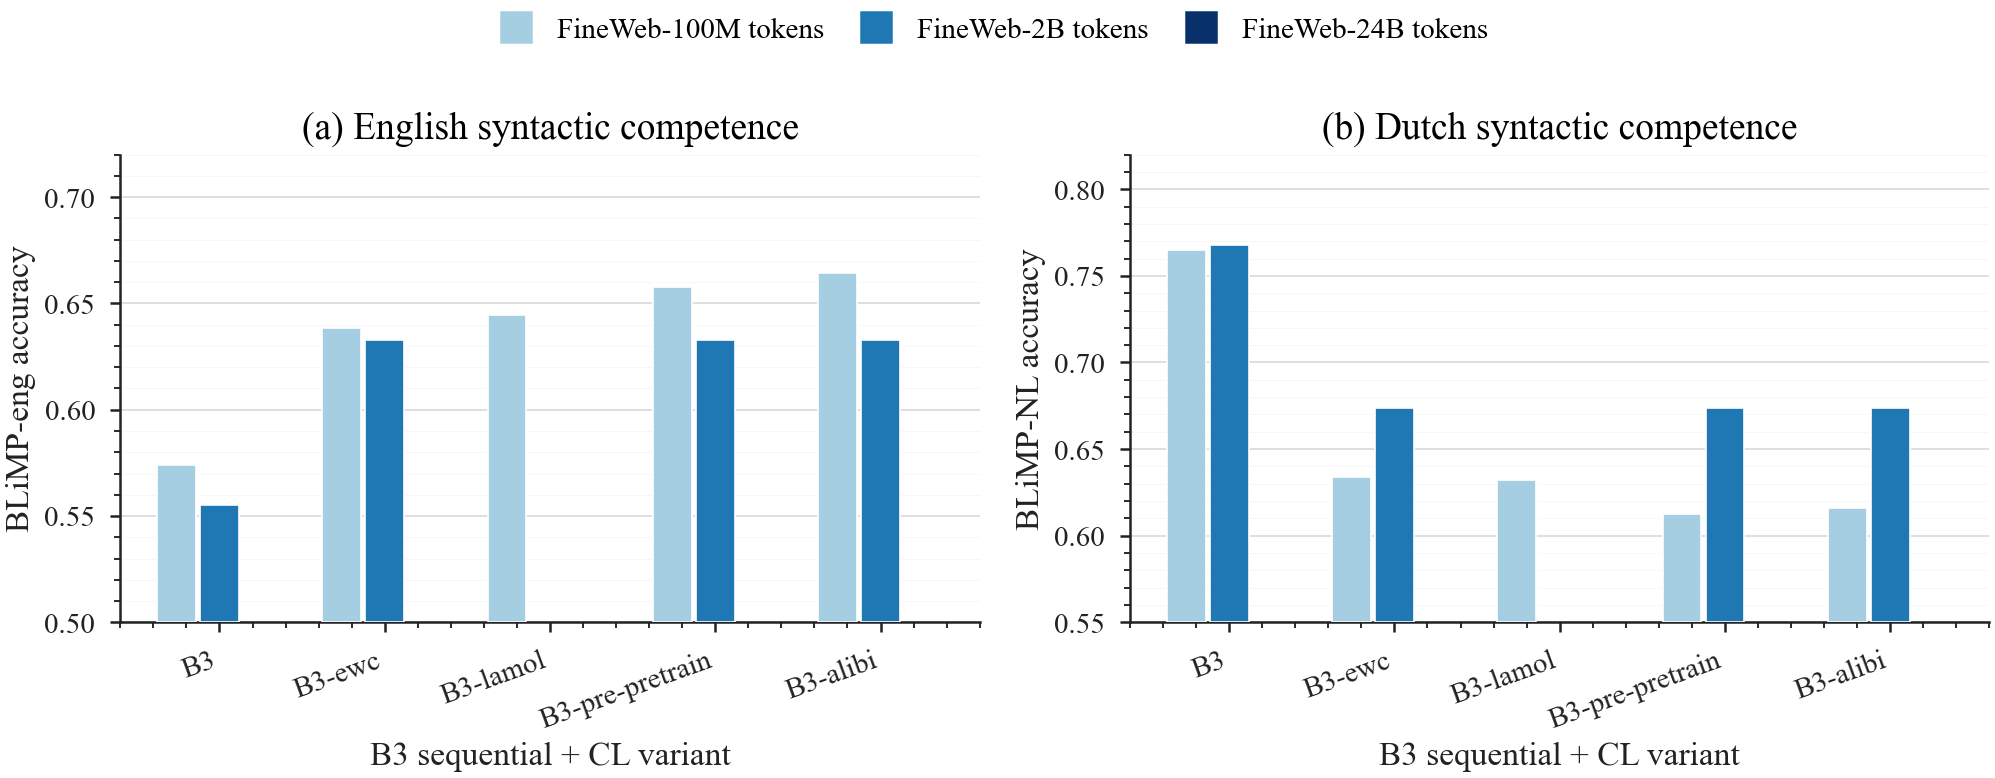
\includegraphics[width=1\linewidth]{fig/fig_cl_variants_scaling.png}
    \caption{Enter Caption}
    \label{fig:placeholder}
\end{figure}



\newpage

\section{Supplementary MECO Figures}\label{sec:meco-figs-supp}


\begin{figure}
    \centering
    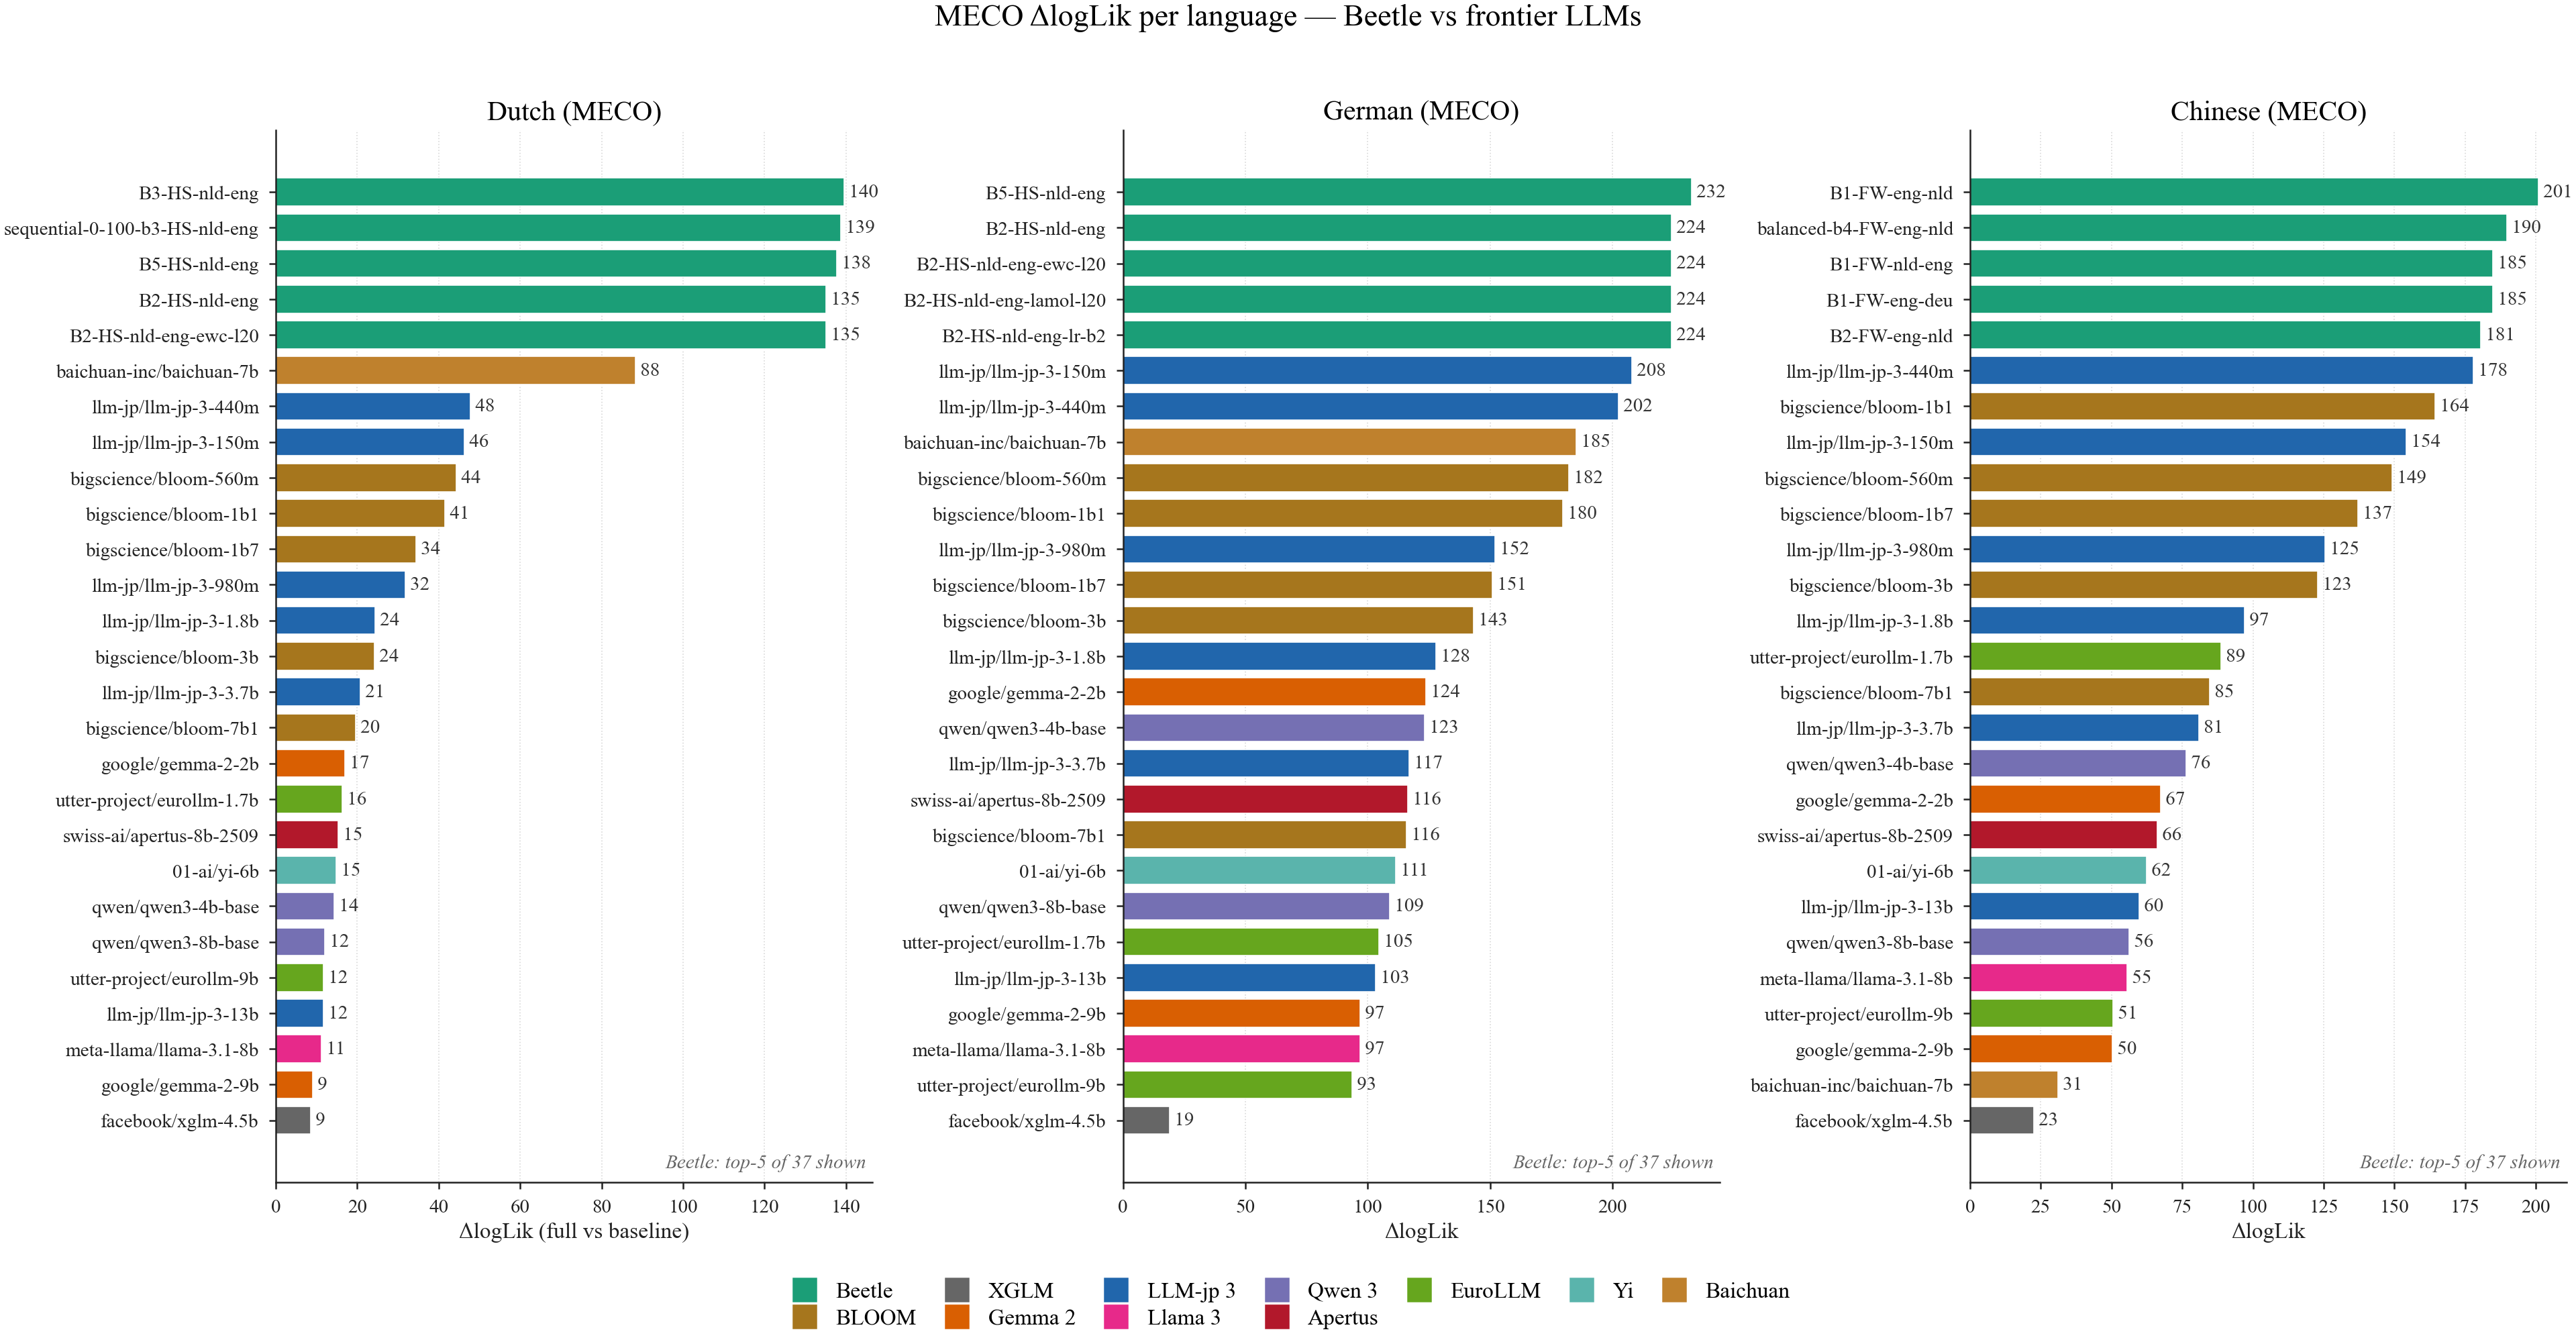
\includegraphics[width=1\linewidth]{fig/fig_meco_beetle_vs_baselines_bars.png}
    \caption{Enter Caption}
    \label{fig:placeholder}
\end{figure}


\begin{figure}
    \centering
    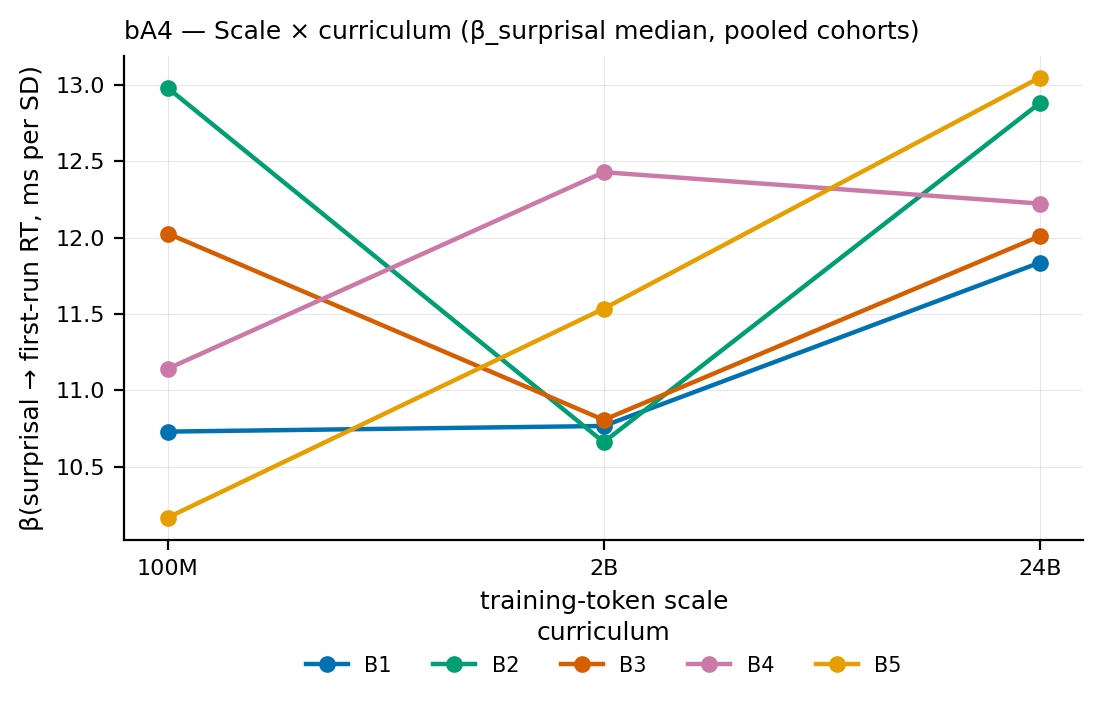
\includegraphics[width=1\linewidth]{fig/meco/bA4_scale_x_curriculum.png}
    \caption{Enter Caption}
    \label{fig:placeholder}
\end{figure}


\begin{figure}
    \centering
    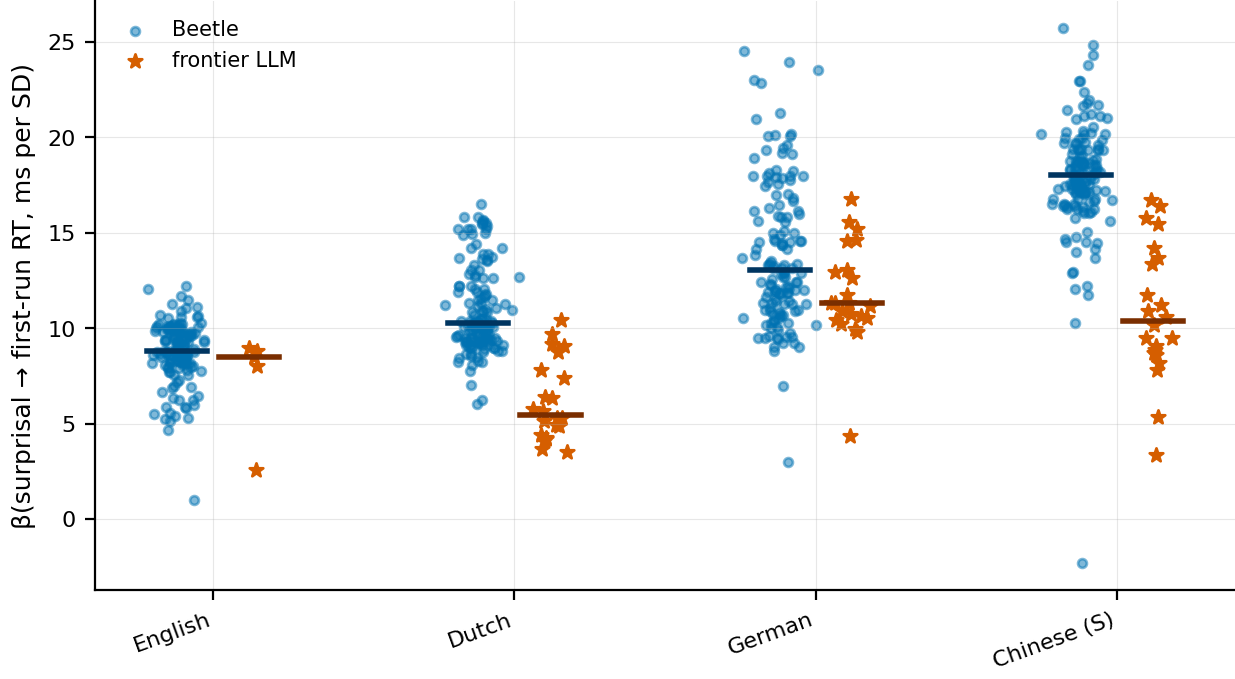
\includegraphics[width=1\linewidth]{fig/meco/bA5_beetle_vs_llm.png}
    \caption{Enter Caption}
    \label{fig:placeholder}
\end{figure}



\begin{figure}
    \centering
    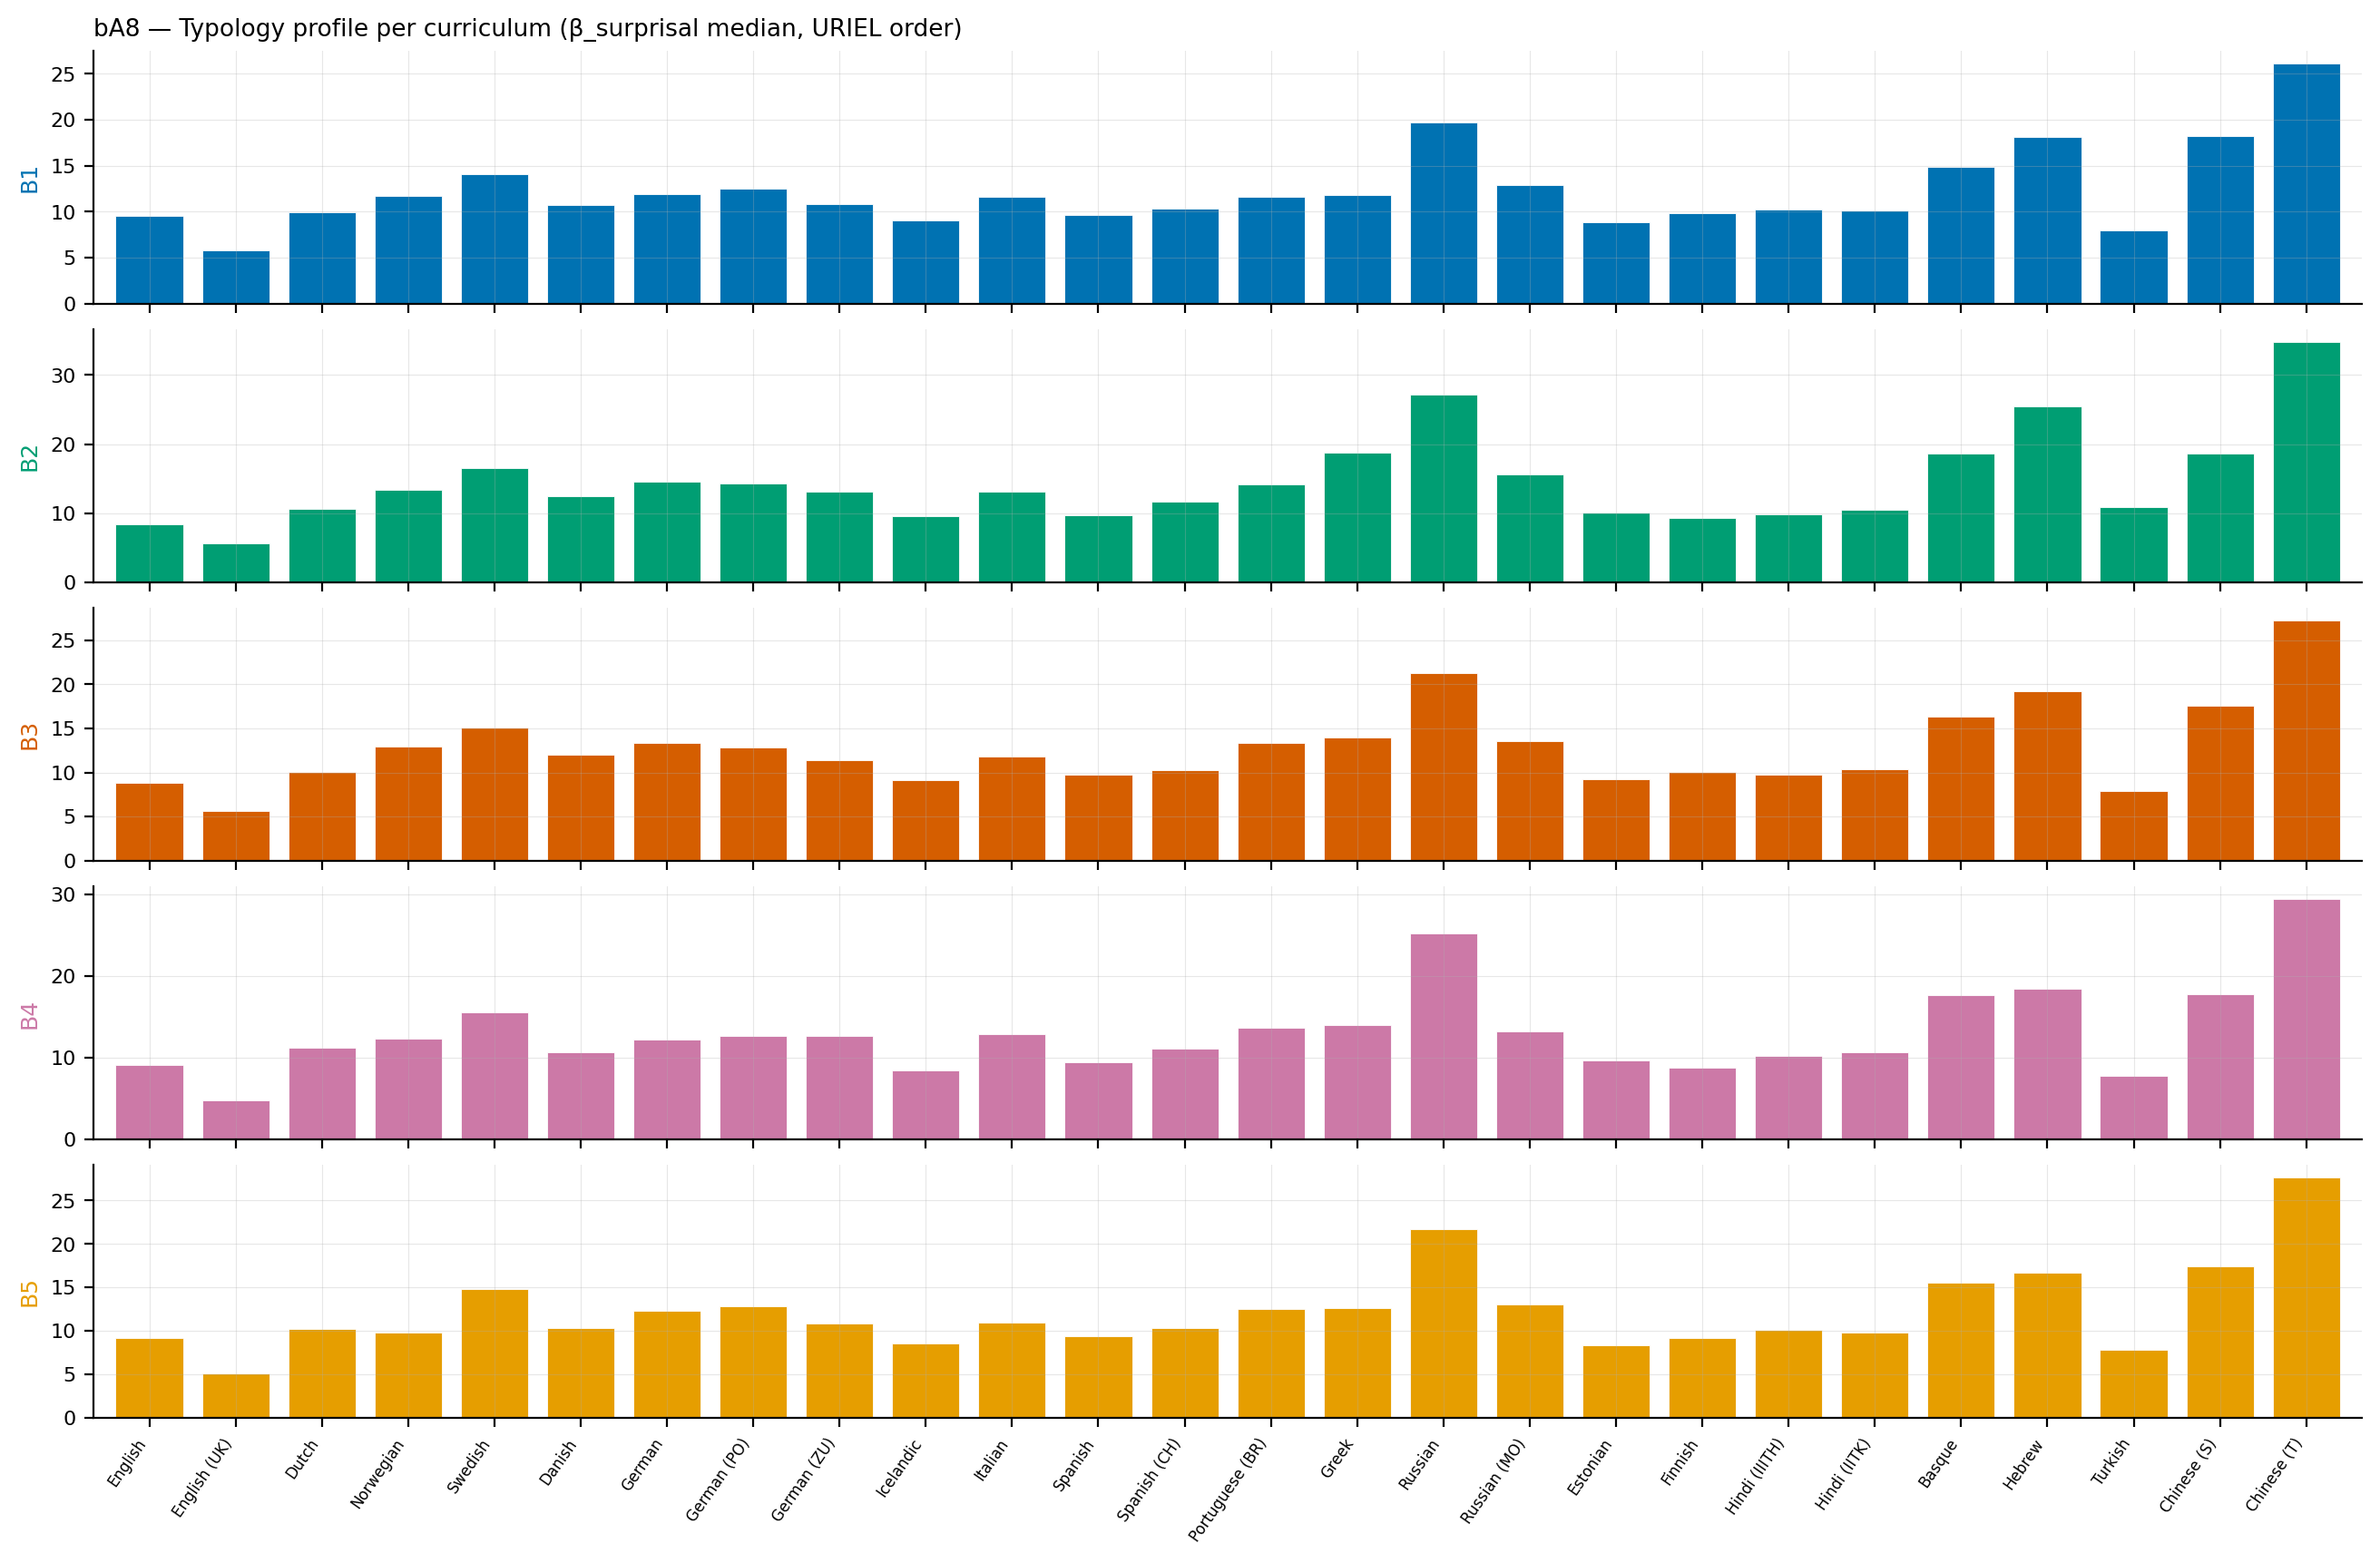
\includegraphics[width=1\linewidth]{fig/meco/bA8_typology_per_curriculum.png}
    \caption{Enter Caption}
    \label{fig:placeholder}
\end{figure}

\begin{figure}
    \centering
    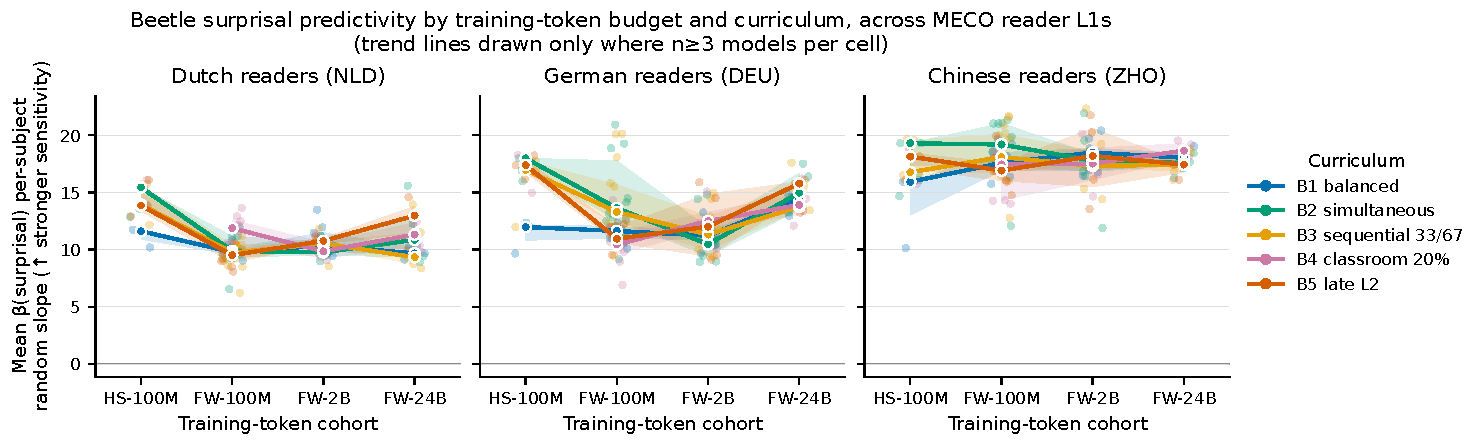
\includegraphics[width=1\linewidth]{fig/meco/fig1_scaling_x_curriculum.pdf}
    \caption{Enter Caption}
    \label{fig:placeholder}
\end{figure}

\begin{figure}
    \centering
    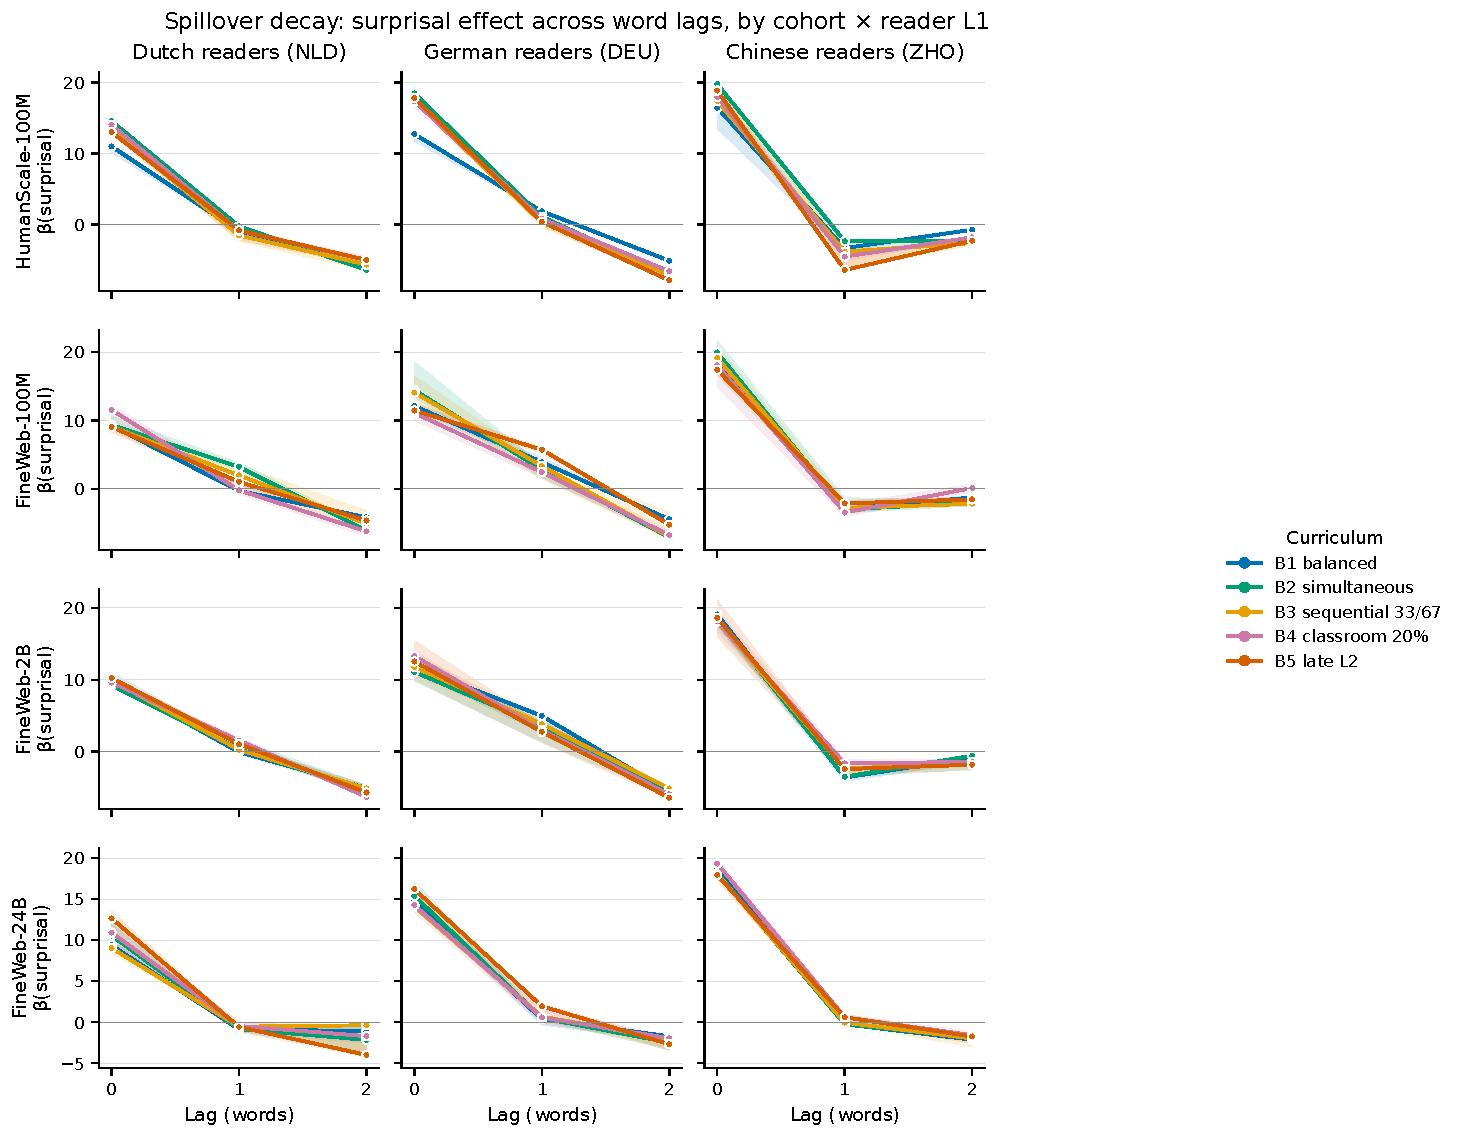
\includegraphics[width=1\linewidth]{fig/meco/fig3_spillover_decay.pdf}
    \caption{Enter Caption}
    \label{fig:placeholder}
\end{figure}



\begin{figure}
    \centering
    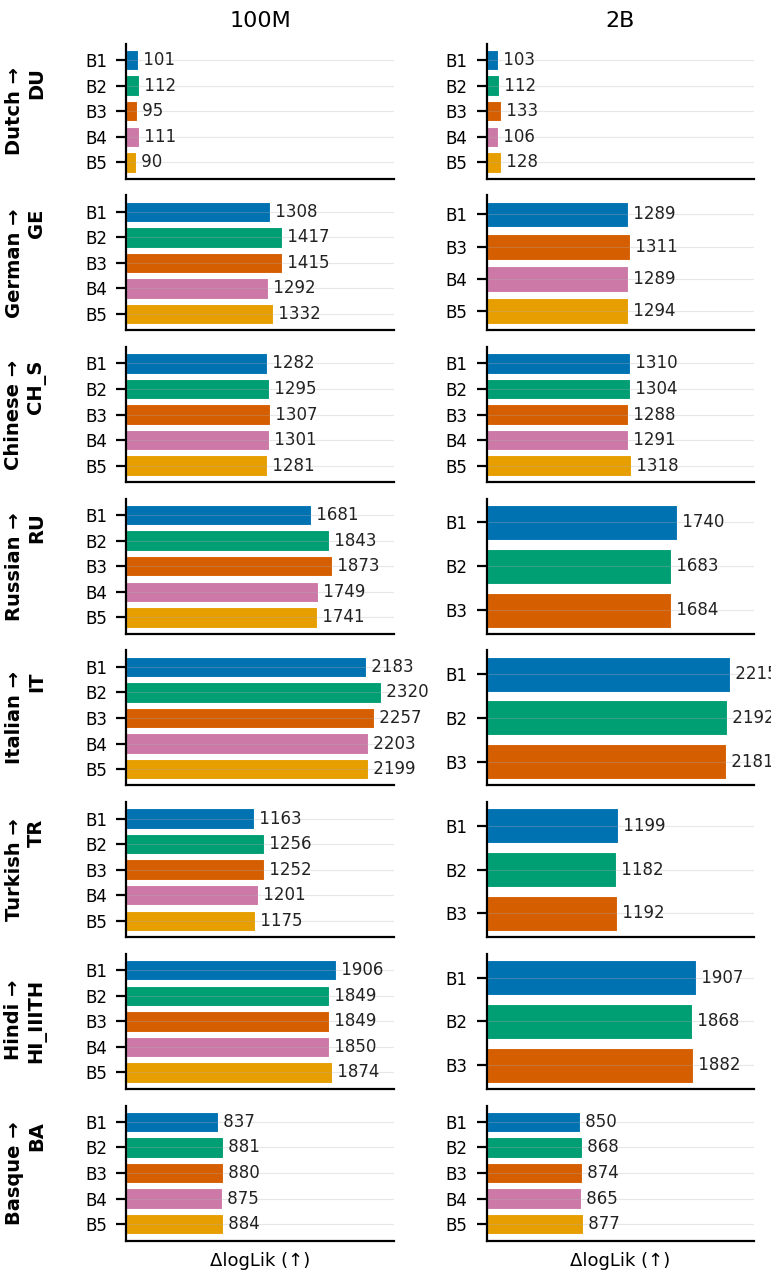
\includegraphics[width=0.8\linewidth]{fig/meco/fig9b_curriculum_sweep_matched.png}
    \caption{Enter Caption}
    \label{fig:placeholder}
\end{figure}




\newpage 


\begin{table}[!ht]
\centering
\begin{tabular}{lccccccc}
\hline
Strategy & BLiMP-en (\%) & BLiMP-nl (\%) & BLiSS RP@0 & BLiSS RP@$\tau$ & BLiSS NGS & BLiSS CPS & MECO \\
\hline
base& 63.86 & 63.51 & 55.96 & 48.35 & 55.88 & 49.49 & 5.135 \\
ewc & 63.83 & 63.37 & 56.64 & 48.58 & 56.02 & 50.62 & 5.136 \\
lamol & 64.46 & 63.24 & 54.60 & 48.81 & 55.47 & 50.06 & 5.143 \\
pre-pretrain & 65.77 & 61.28 & 57.66 & 49.72 & 55.93 & 47.79 & 4.989 \\
alibi & 66.43 & 61.59 & 56.19 & 49.83 & 55.72 & 49.94 & 5.060 \\
\hline
\end{tabular}
\caption{Performance comparison across different training strategies.}
\label{tab:strategy_results}
\end{table}



\section{BLiSS Curriculum, Token Efficiency, and Metric Tradeoff}\label{sec:bliss-detail}

\begin{figure}[!ht]
  \centering
  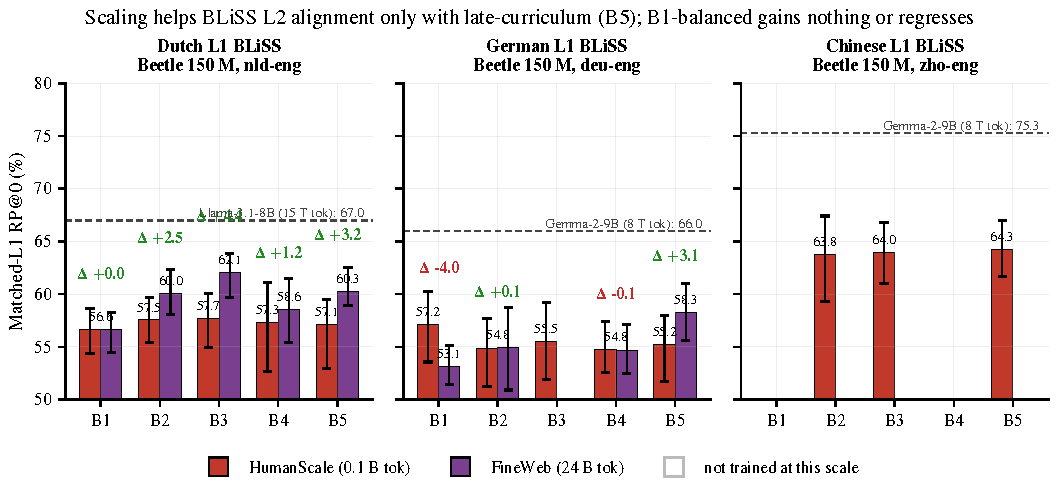
\includegraphics[width=\linewidth]{fig/F7_bliss_curriculum_x_scale.pdf}
  \caption{BLiSS NGS by exposure curriculum (B1--B5) $\times$ training scale (\textsc{HumanScale}~100M, \textsc{FineWeb}~2B). Unlike MECO, simultaneous (B2) and balanced (B1) schedules dominate at FineWeb scale; late-onset B5 is competitive at HumanScale. BLOOM and XGLM baselines are shown; \textsc{Beetle} FineWeb models surpass the BLOOM-7b1 NGS at both scales.}
  \label{fig:bliss_curriculum_scale}
\end{figure}

\begin{figure}[!ht]
  \centering
  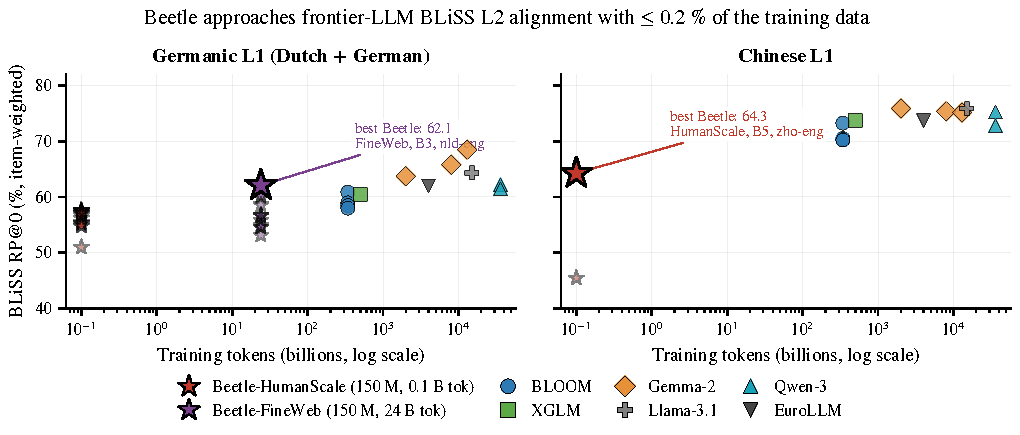
\includegraphics[width=\linewidth]{fig/F6_bliss_token_efficiency.pdf}
  \caption{BLiSS NGS as a function of training tokens for \textsc{Beetle} models (nld--eng, B1--B5) vs.\ baselines. Simultaneous B2 and balanced B1 reach competitive NGS earlier than sequential / late schedules --- the \emph{reverse} of the MECO token-efficiency ordering (Fig.~\ref{fig:meco_efficiency}).}
  \label{fig:bliss_efficiency}
\end{figure}

\begin{figure}[!ht]
  \centering
  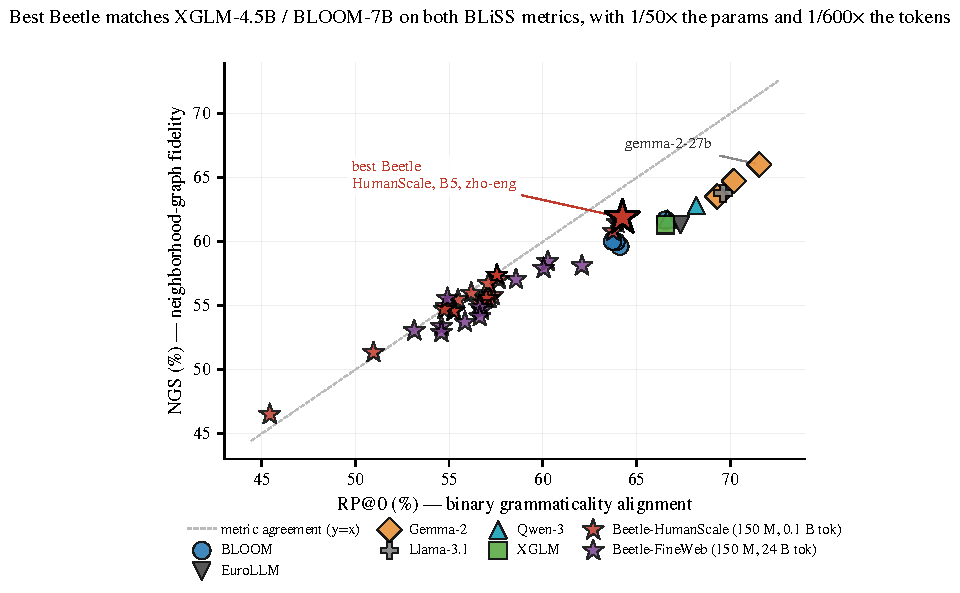
\includegraphics[width=\linewidth]{fig/F8_bliss_metric_tradeoff_pareto.pdf}
  \caption{BLiSS metric tradeoff: NGS vs.\ CPS vs.\ RP$@\tau$ across \textsc{Beetle} curricula and baselines. \textsc{Beetle} FineWeb B5 nld--eng leads NGS at \textbf{64.9} and RP$@0$ at \textbf{68.5}; XGLM-4.5B leads CPS at 59.1.}
  \label{fig:bliss_pareto}
\end{figure}


\newpage 
\section{Pedagogical Utility and CEFR Stratification}\label{sec:pedagogical-detail}

\begin{figure}[!ht]
  \centering
  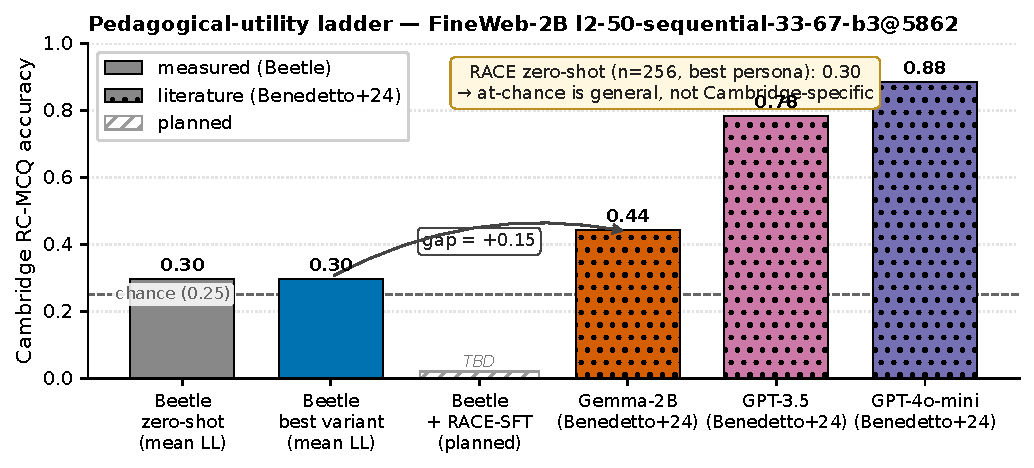
\includegraphics[width=\linewidth]{fig/P3_pedagogical_utility_ladder.pdf}
  \caption{\textbf{Pedagogical-utility ladder.} Cambridge CUP\&A5 RC-MCQ accuracy: Beetle zero-shot vs.\ Beetle best variant vs.\ Gemma-2B / GPT-3.5 / GPT-4o-mini reference rows from \citet{benedetto-etal-2024-using}. The Beetle-RACE-SFT bar is reserved (App.~\ref{sec:roadmap}, item 4) and rendered as a hatched placeholder.}
  \label{fig:ped_ladder}
\end{figure}

\begin{figure}[!ht]
  \centering
  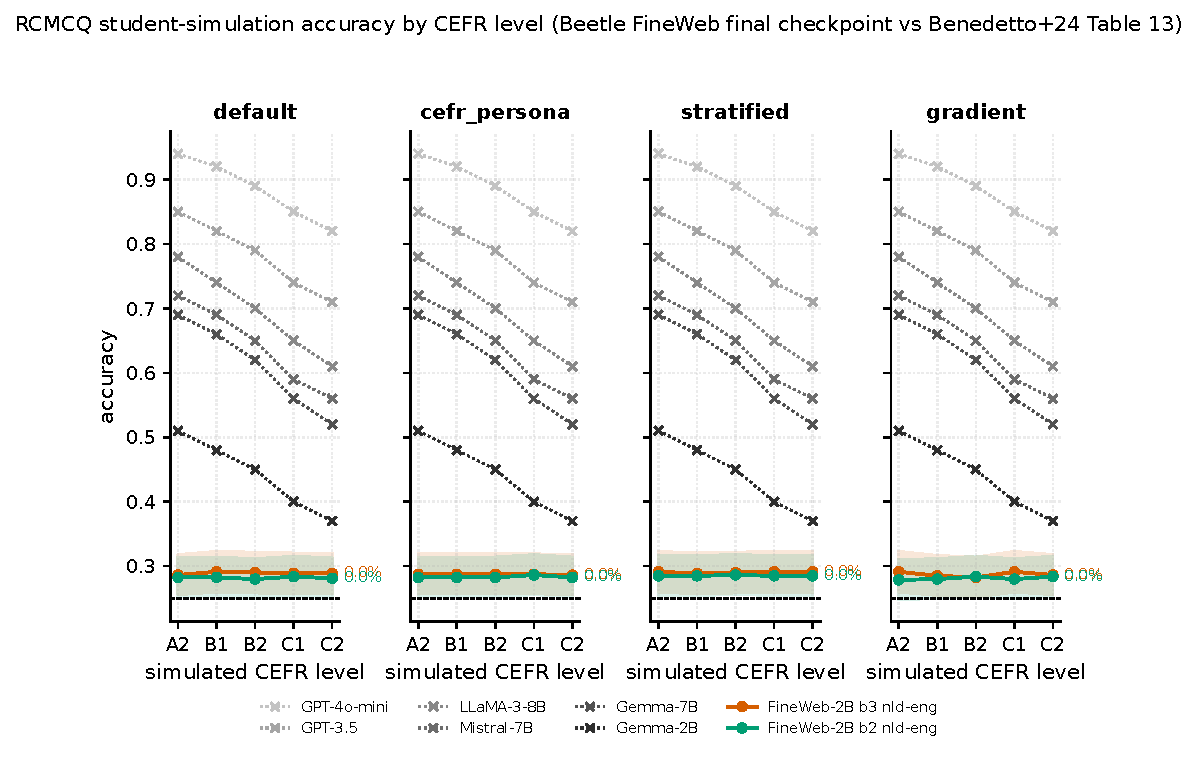
\includegraphics[width=\linewidth]{fig/P5_rcmcq_cefr.pdf}
  \caption{\textbf{CEFR stratification.} CEFR-stratified RC-MCQ accuracy under four prompting variants: \textsc{Beetle} FineWeb-2B B2/B3 vs.\ the six LLM rows of \citet{benedetto-etal-2024-using}. Beetle exhibits CEFR-monotonic behaviour on a subset of prompting variants.}
  \label{fig:rcmcq_cefr}
\end{figure}

\section{FLORES-200 Convergence Detail}\label{sec:flores-detail}

\begin{figure*}[!ht]
  \centering
  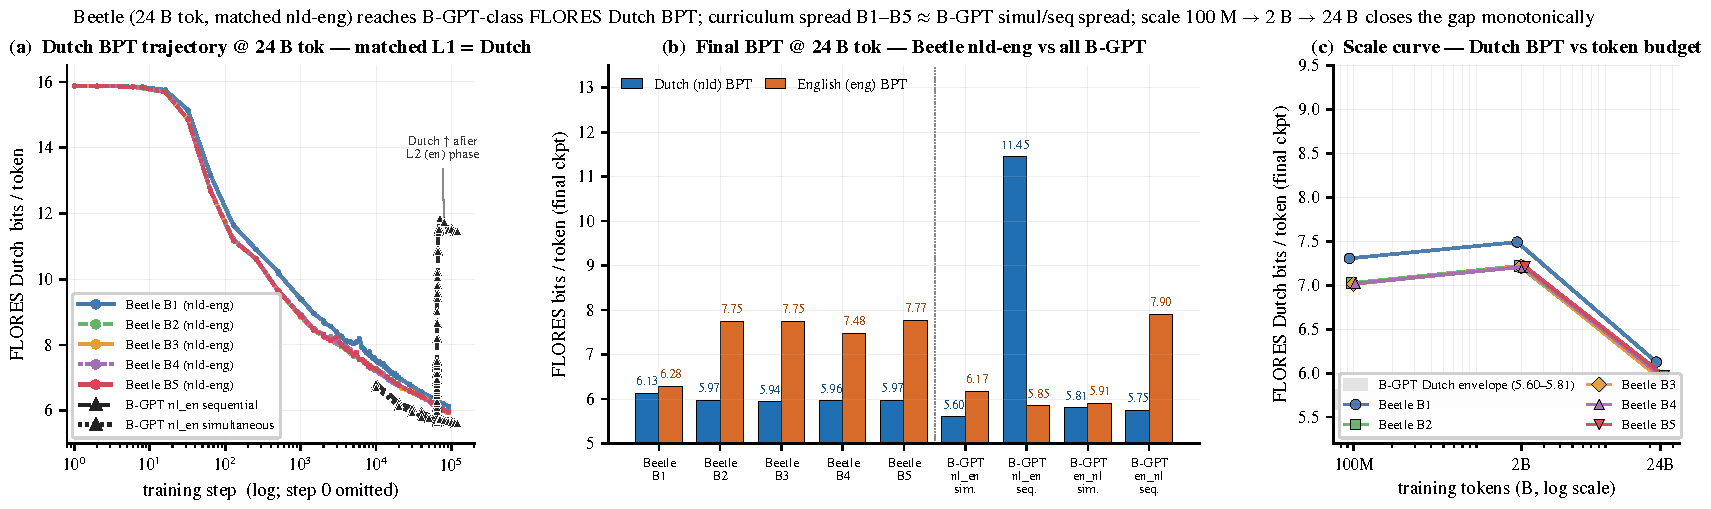
\includegraphics[width=\linewidth]{fig/F10_flores_beetle_vs_bgpt.pdf}
  \caption{\textbf{Bits-per-byte FLORES, Beetle vs.\ B-GPT (matched nld--eng).} (a) Dutch FLORES BPB trajectory across log-spaced \textsc{Beetle} training steps for the FineWeb-24B nld--eng cohort (B1--B5); the B-GPT non-forgetting envelope is drawn as a horizontal band because B-GPT checkpoints are not log-spaced. (b) Final-checkpoint Dutch / English FLORES paired bars at 24~B tokens for \textsc{Beetle} B1--B5 plus all four B-GPT variants. (c) Scale curve: final Dutch BPB versus 100~M / 2~B / 24~B token budget per curriculum, with the B-GPT non-forgetting envelope shaded. The matched-bilingual \textsc{Beetle} converges into the B-GPT band as the token budget grows; only the B-GPT \textsc{nl-en} sequential variant exhibits Dutch catastrophic forgetting (11.45 BPT).}
  \label{fig:flores_beetle_vs_bgpt}
\end{figure*}



\section{\beetle{} Control Parameters}\label{sec:beetle-control-parameters}

\paragraph{Exposure Schedules} For bilingual and trilingual experiments, language mixing is governed by one of six \emph{curriculum schedules} that modulate the per-step proportion of L1, L2, and (for trilingual runs) L3 tokens. The schedules – \textbf{balanced}, \textbf{late}, \textbf{sequential}, \textbf{heritage}, \textbf{part\_time}, and \textbf{simultaneous} – summarised in \textit{Table} \ref{tab:curricula} attempt to the space from fully interleaved exposure (modelling balanced bilingual/trilingual acquisition) to sequential exposure (modelling a more extreme acquisition scenario where learners receive no L1 input upon the acquisition of L2 in a bilingual setting; or not L1 and L2 input upon the acquisition of L3).

\subsection{Control Parameters}

All continual-learning experiments fix the language order to English~$\to$~Dutch~$\to$~Chinese under a uniform trilingual \texttt{sequential} exposure schedule, using the same PicoDecoder architecture and training budget as the main sweep ($T_{\max}\!=\!30{,}578$ steps). For EWC, we vary the regularisation strength $\lambda\!\in\!\{5,\,20,\,50,\,150\}$; the values $\lambda\!=\!20$ and $\lambda\!=\!150$ replicate settings reported in \citep{constantinescu2025investigating}.  The Fisher diagonal $\hat{F}$ is estimated on $K\!=\!10$ held-out L1 batches at the L1$\to$L2 phase boundary, and the anchor parameters~$\theta^*$ are snapshotted at the same moment; the penalty is then active for the remainder of training. For MAML, we vary the hybrid ratio $r\!\in\!\{0.25,\,0.50,\,0.75,\,1.00\}$, which controls the fraction of training steps executed as $N$-way, $K$-shot meta episodes ($N\!=\!5$, $K\!=\!1$, 3 inner SGD steps at $\alpha\!=\!0.1$) versus standard autoregressive steps. We have a combined condition that combines all four EWC strengths with all four hybrid ratios, yielding a $4\!\times\!4$ factorial design, which we compare against a trilingual baseline, producing 25 experimental conditions, each trained and evaluated identically to the baseline trilingual run.

%\paragraph{Multilingual Data Quality} We use FineWeb2 \citep{penedo2025fineweb2} for 2B tokens of bilingual model pretraining for the following languages: English, Japanese, Chinese, French, German, (Italian), Basque, Turkish, Indonesian. We do data decontamination.  \textit{ignore for potential CDL submission}


\subsection{Meta-Learning}

\beetle{}  uses the \texttt{pico-maml} implementation of MAML used in \citet{africa-etal-2025-learning} and \citet{africa-etal-2025-meta}. 


\begin{algorithm}\small \caption{Distributed SMLMT Loop}\label{alg:dist-maml} \begin{algorithmic} \State Initialize model $f_\theta$, head $h_\phi$, outer optimizer, and inner SGD on $h_\phi$ \State step $\leftarrow 0$ \For{each sub-batch $B$ from dataloader} \State $X \leftarrow \text{AllGather}(B\ \text{inputs})$ \Comment{across devices} \State $r \leftarrow \text{Broadcast}(\text{Uniform}(0,1))$ \If{$r < \rho$} \State $(S,Q,y_S,y_Q) \leftarrow \text{MaskTokens}(X)$ \State $\phi_{\text{snap}} \leftarrow \phi$ \Comment{save head params} \For{$t = 1$ to $T_{\text{inner}}$} \State $\ell_S \leftarrow \text{CE}\big(h_\phi(f_\theta(S)),,y_S\big)$ \State $\phi \leftarrow \phi - \alpha,\nabla_\phi \ell_S$ \EndFor \State $\ell \leftarrow \text{CE}\big(h_\phi(f_\theta(Q)),,y_Q\big)$ \State $\phi \leftarrow \phi_{\text{snap}}$ \Comment{restore head} \Else \State $X_{\text{in}} \leftarrow X$ without last token; $Y \leftarrow X$ without first token \State $\ell \leftarrow \text{CE}\big(f_\theta(X_{\text{in}}),,Y\big)$ \EndIf \State Backward$\big(\ell ,/, \text{accum\_steps}\big)$ \If{$( \text{step} + 1 ) \bmod \text{accum\_steps} = 0$} \State OptimizerStep(); SchedulerStep(); ZeroGrad() \State AggregateMetrics($\ell$); Barrier() \EndIf \State step $\leftarrow$ step $+ 1$ \EndFor \end{algorithmic} \end{algorithm}

\begin{algorithm}\small \caption{Distributed AR Loop}\label{alg:dist-ar} \begin{algorithmic} \State Initialize configs, Fabric/strategy, tokenizer, model $f_\theta$, optimizer \State Prepare dataloader and distribute it \State step $\leftarrow 0$; ZeroGrad() \For{each sub-batch $B$ from dataloader} \State $X \leftarrow \text{AllGather}(B\ \text{inputs})$ \Comment{across devices} \State $X_{\text{in}} \leftarrow X$ without last token; $Y \leftarrow X$ without first token \State $\ell \leftarrow \text{CE}\big(f_\theta(X_{\text{in}}),,Y\big)$ \State Backward$\big(\ell ,/, \text{accum\_steps}\big)$ \If{$( \text{step} + 1 ) \bmod \text{accum\_steps} = 0$} \State OptimizerStep(); SchedulerStep(); ZeroGrad() \State Barrier() \Comment{optional} \EndIf \State step $\leftarrow$ step $+ 1$ \EndFor \end{algorithmic} \end{algorithm}


\newpage 

\section{Learning Dynamics}

\begin{figure}
    \centering
    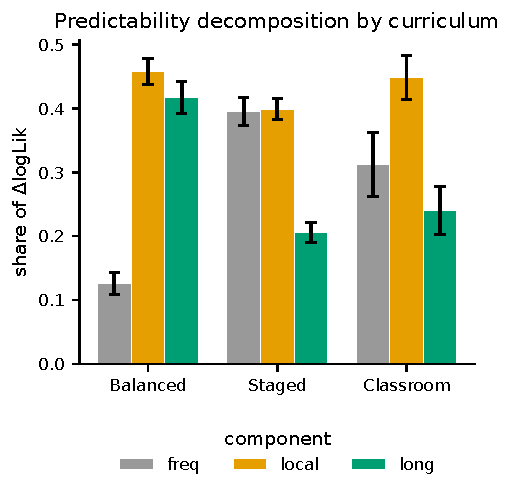
\includegraphics[width=1\linewidth]{fig/interp/D5_decomp_shares.pdf}
    \caption{Enter Caption}
    \label{fig:placeholder}
\end{figure}

\begin{figure}
    \centering
    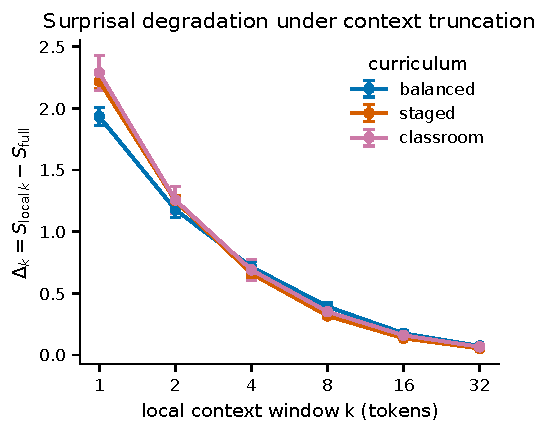
\includegraphics[width=1\linewidth]{fig/interp/D6_context_degradation.pdf}
    \caption{Enter Caption}
    \label{fig:placeholder}
\end{figure}

\begin{figure}
    \centering
    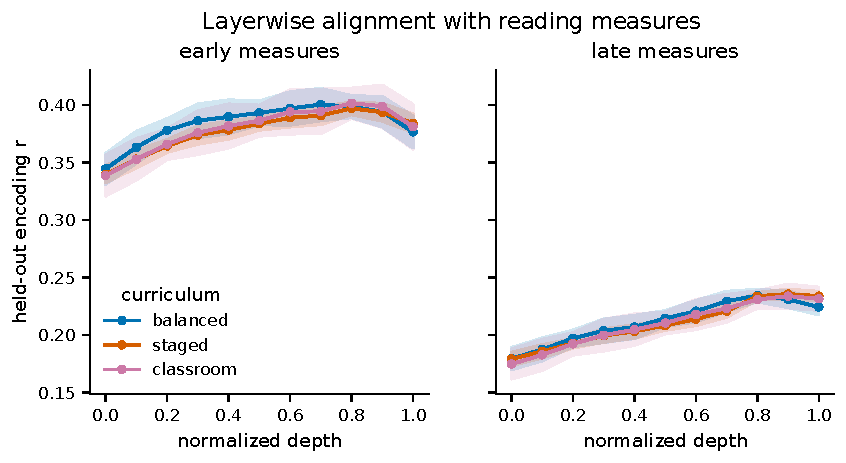
\includegraphics[width=1\linewidth]{fig/interp/D8_layerwise_profile.pdf}
    \caption{Enter Caption}
    \label{fig:placeholder}
\end{figure}


\begin{figure}
    \centering
    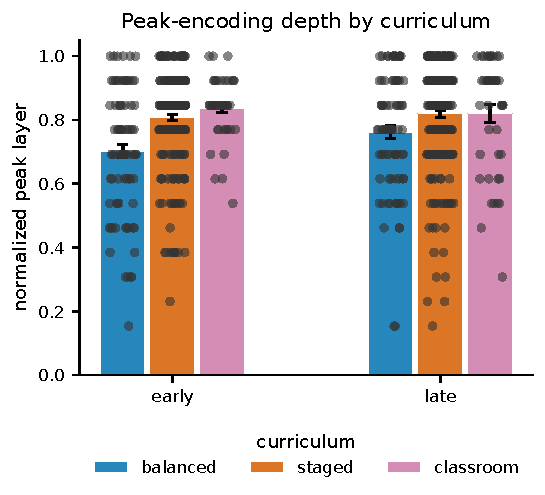
\includegraphics[width=1\linewidth]{fig/interp/D9_peak_layer.pdf}
    \caption{Enter Caption}
    \label{fig:placeholder}
\end{figure}



\begin{figure}
    \centering
    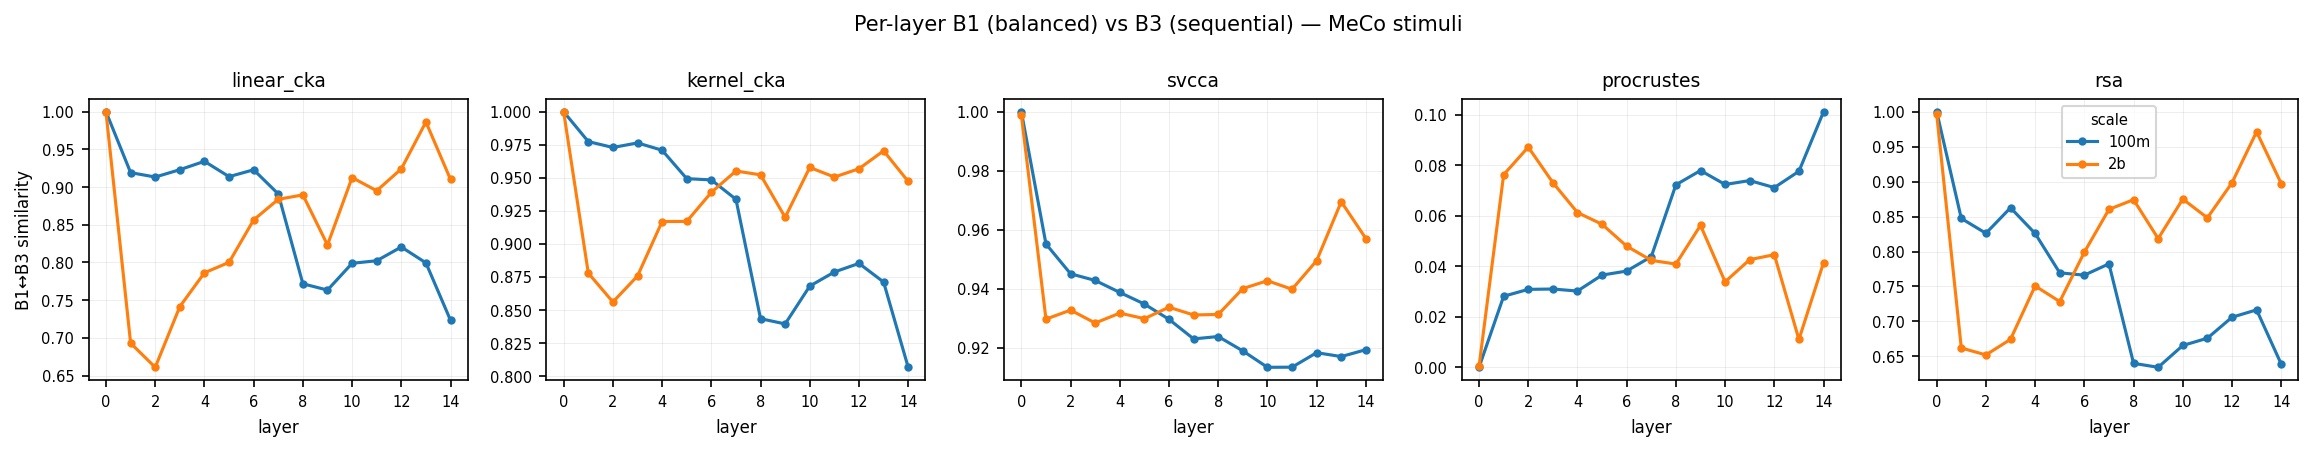
\includegraphics[width=1\linewidth]{fig/interp/repsim_b1_vs_b3.png}
    \caption{Enter Caption}
    \label{fig:placeholder}
\end{figure}

\begin{figure}
    \centering
    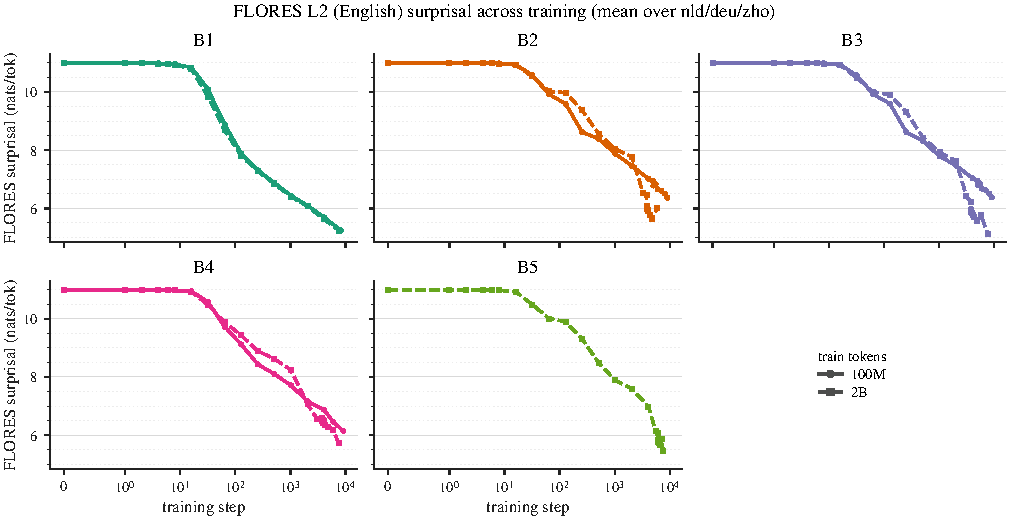
\includegraphics[width=1\linewidth]{fig/flores/fig_flores_main.pdf}
    \caption{Enter Caption}
    \label{fig:placeholder}
\end{figure}

\begin{figure}
    \centering
    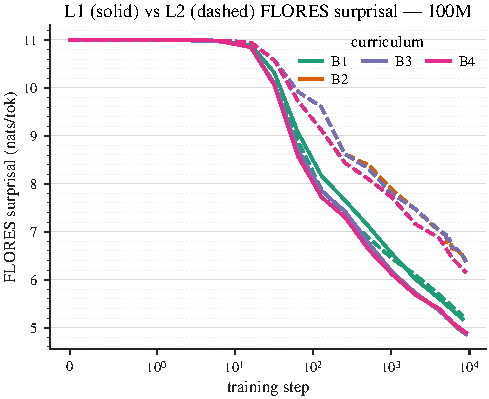
\includegraphics[width=1\linewidth]{fig/flores/fig_flores_l1l2.pdf}
    \caption{Enter Caption}
    \label{fig:placeholder}
\end{figure}


\begin{figure}
    \centering
    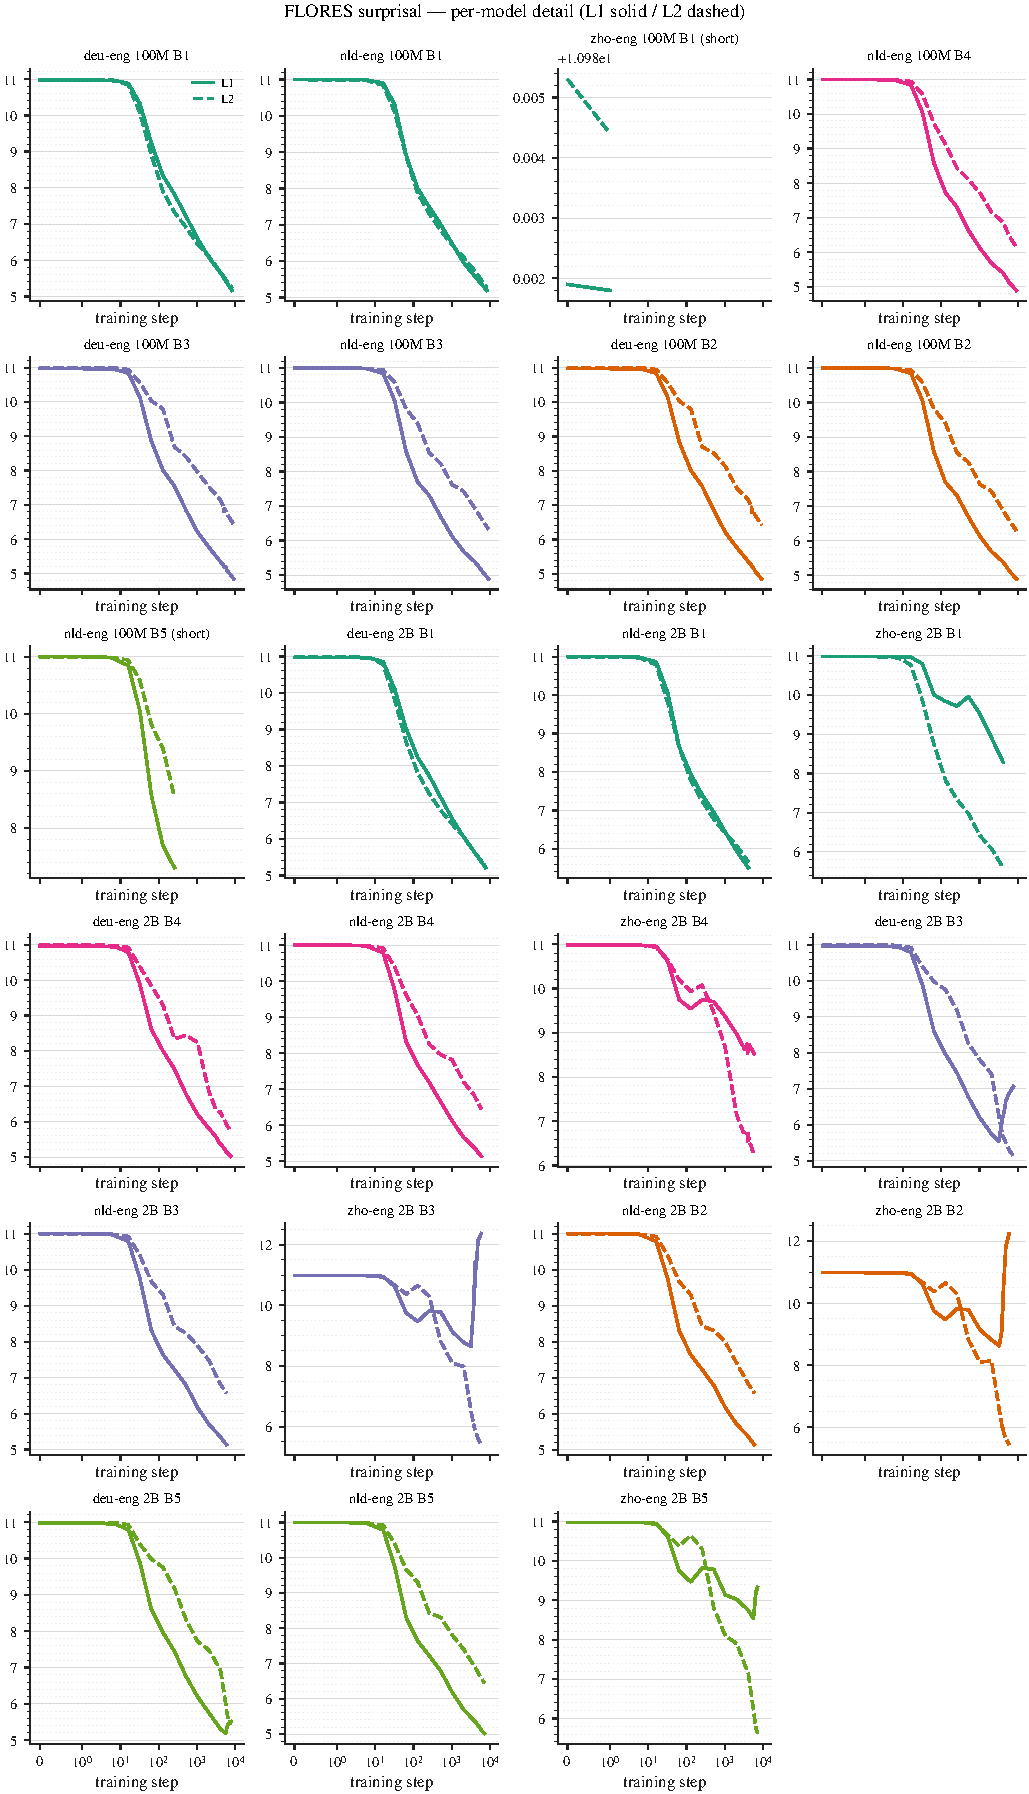
\includegraphics[width=1\linewidth]{fig/flores/appx_flores_per_model.pdf}
    \caption{\suchir{TO DO retrain zho-100m B1}}
    \label{fig:placeholder}
\end{figure}


\subsection{Q1 --- How does interpretability differ between models?}\label{sec:pico-q1}

\begin{figure}[!ht]
  \centering
  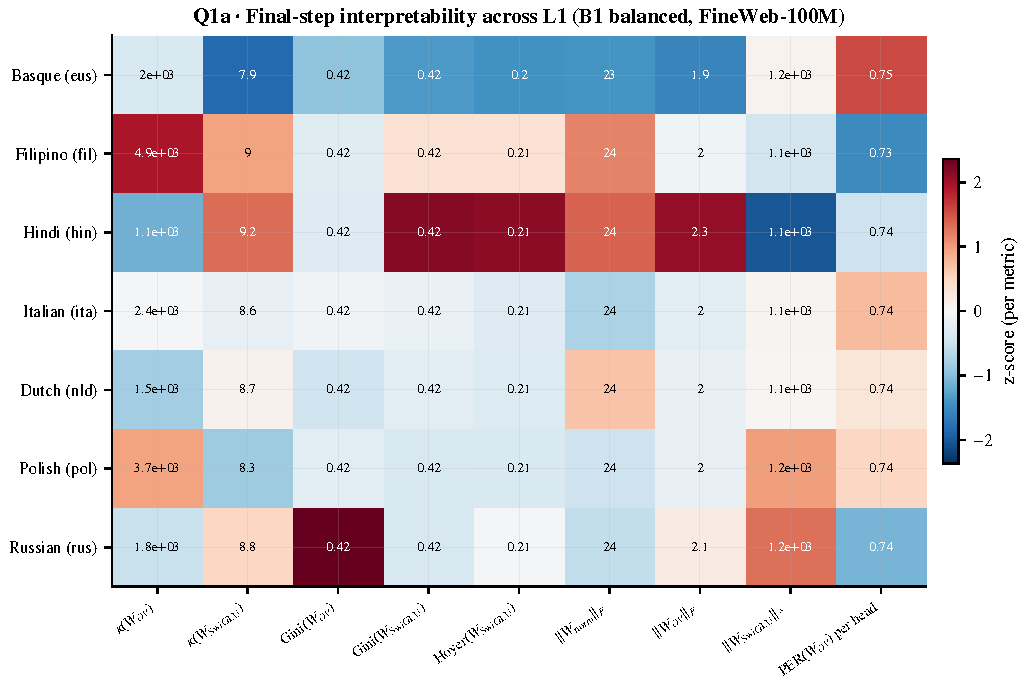
\includegraphics[width=\linewidth]{fig/pico_q1a_l1_heatmap.pdf}
  \caption{\textbf{Q1a -- L1 heatmap.} Final-step layer-mean of every \textsc{Pico-Analyze} interpretability metric against every L1 (B1 only). Cell colour is the per-metric $z$-score; cell text is the raw value. The dominant cross-L1 signal sits in $\kappa(W_{OV})$, which spans an order of magnitude (Dutch $\sim\!1.5\!\times\!10^{3}$ to Hindi $\sim\!1.1\!\times\!10^{4}$). Other metrics are nearly flat across L1 despite the L1s spanning four typological groupings (Germanic, Romance, Slavic, Indo-Aryan, Austronesian, isolate), suggesting that the OV-circuit's spectral conditioning encodes typological distance from the L2 (English) far more sensitively than any sparsity-style metric does.}
  \label{fig:pico-q1a}
\end{figure}

\begin{figure}[!ht]
  \centering
  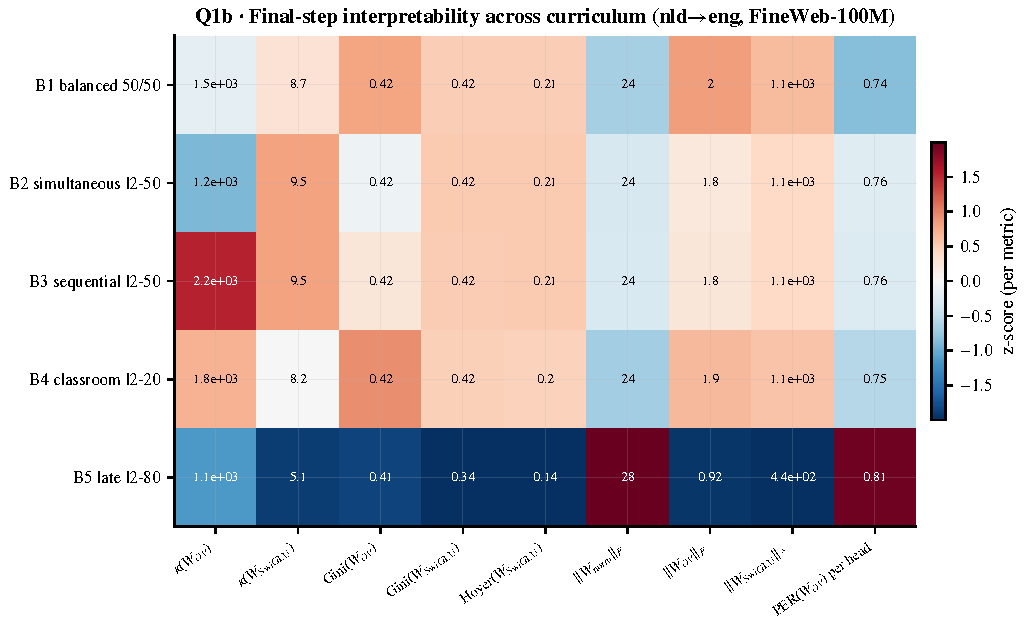
\includegraphics[width=\linewidth]{fig/pico_q1b_curriculum_heatmap.pdf}
  \caption{\textbf{Q1b -- Curriculum heatmap.} Same construction as Fig.~\ref{fig:pico-q1a}, sliced over the nld--eng curriculum sweep (B1--B5). B5 (late l2-80) is the standout outlier on \texttt{gini-swiglu}, \texttt{hoyer-swiglu}, $\Vert W_{OV}\Vert_F$ and $\Vert W_{\text{SwiGLU}}\Vert_*$: its SwiGLU weights are markedly less sparse and the OV norm is depressed (0.92 vs.\ $\sim\!1.78$--$2.02$ for B1--B4). Delaying L2 exposure to 80\% of training prevents the OV circuit from acquiring the high-norm, high-sparsity geometry the other curricula reach.}
  \label{fig:pico-q1b}
\end{figure}

\begin{figure}[!ht]
  \centering
  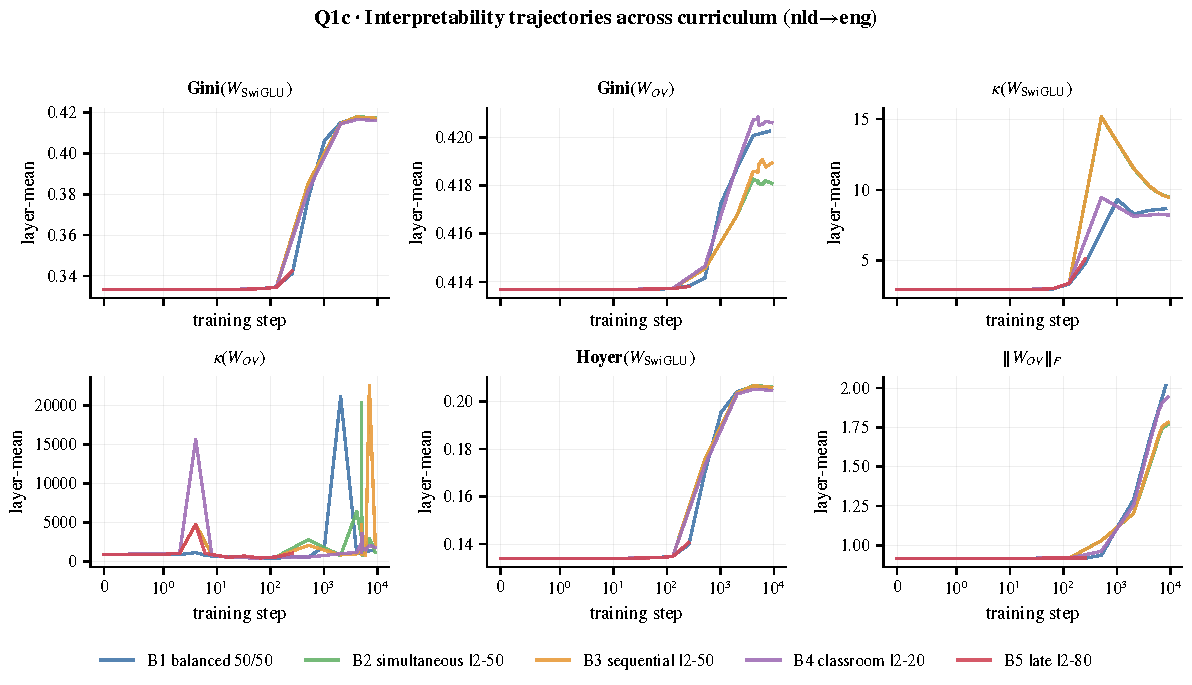
\includegraphics[width=\linewidth]{fig/pico_q1c_curriculum_trajectories.pdf}
  \caption{\textbf{Q1c -- Curriculum trajectories.} Layer-mean trajectories across training step for the B1--B5 nld--eng curricula on six representative interpretability metrics. All metrics emerge between step 256 and 1024 and saturate by 8k; B5 follows the same trajectory shape but at a depressed plateau, indicating that the curriculum effect is one of \emph{plateau height} rather than \emph{onset timing}.}
  \label{fig:pico-q1c}
\end{figure}

\begin{figure}[!ht]
  \centering
  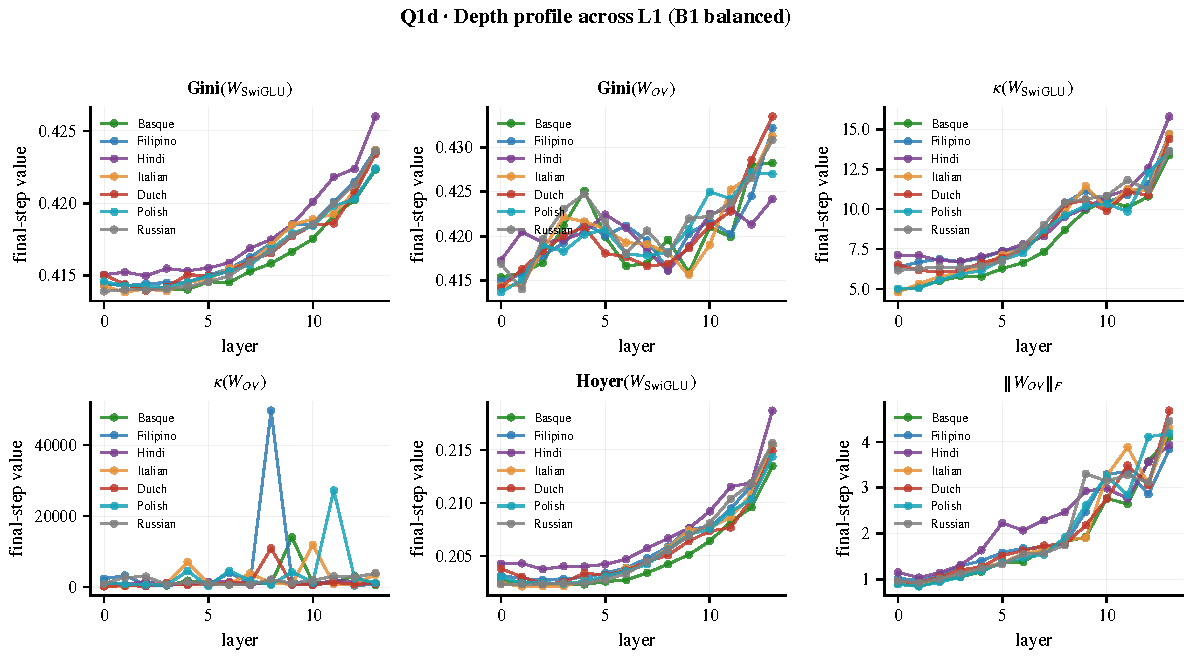
\includegraphics[width=\linewidth]{fig/pico_q1d_depth_profile_l1.pdf}
  \caption{\textbf{Q1d -- Depth profile across L1.} Final-step value as a function of layer index, one panel per metric, lines = L1 (B1 only). The OV-circuit signal is concentrated in mid-to-late layers; sparsity metrics (Gini, Hoyer) are layer-flat. Read together with Fig.~\ref{fig:pico-q1a}, this localises the typological-distance signal to the same depth band that hosts the OV induction circuitry.}
  \label{fig:pico-q1d}
\end{figure}

\begin{figure}[!ht]
  \centering
  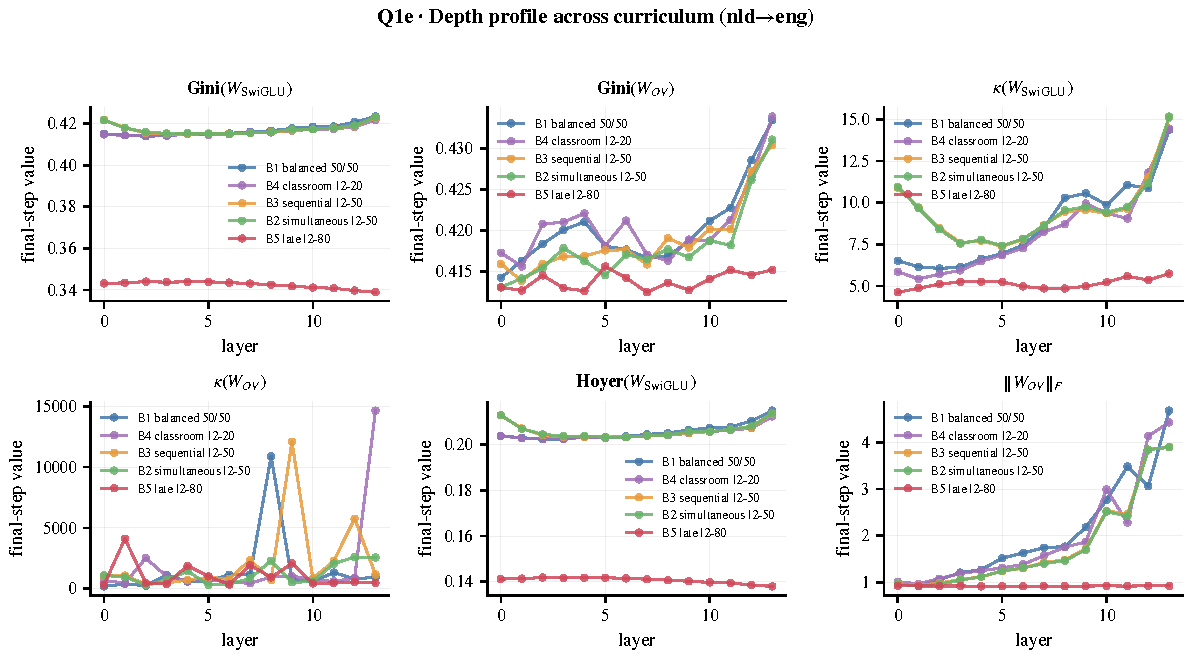
\includegraphics[width=\linewidth]{fig/pico_q1e_depth_profile_curriculum.pdf}
  \caption{\textbf{Q1e -- Depth profile across curriculum.} Same construction as Fig.~\ref{fig:pico-q1d}, lines = curriculum (B1--B5, nld--eng). The B5-vs-B1--B4 plateau gap of Fig.~\ref{fig:pico-q1c} is concentrated in mid-to-late layers, again co-localising with the OV induction band.}
  \label{fig:pico-q1e}
\end{figure}

\subsection{Q2 --- Do interpretability metrics correlate with downstream behaviour?}\label{sec:pico-q2}

\begin{figure}[!ht]
  \centering
  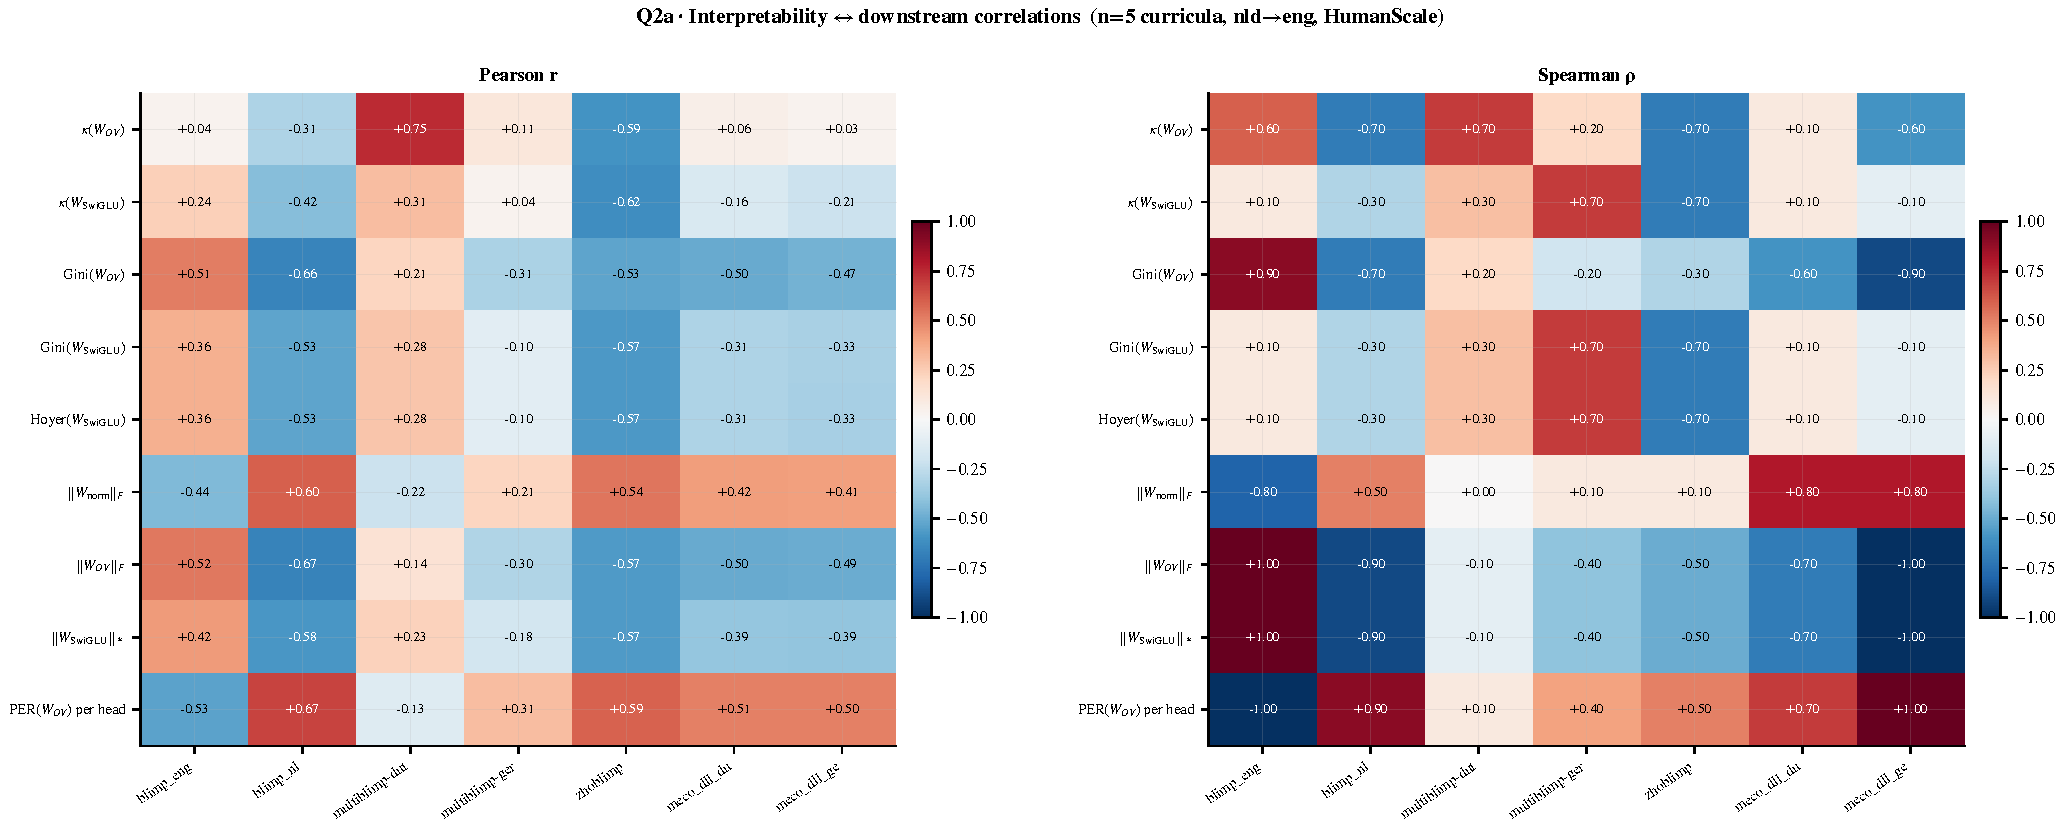
\includegraphics[width=\linewidth]{fig/pico_q2a_corr_heatmap.pdf}
  \caption{\textbf{Q2a -- Correlation heatmap.} Pearson $r$ and Spearman $\rho$ for every (interpretability metric $\times$ downstream metric) pair across the nld--eng curriculum sweep ($n=5$). The signal is asymmetric: sparsity/norm metrics on the OV+SwiGLU subspace track L2 (English) BLiMP performance, but anti-predict the L1-side BLiMP and human-RT alignment. The attention-norm Frobenius $\Vert W_{\text{norm}}\Vert_F$ is the only metric that positively predicts both Dutch BLiMP and MECO surprisal-fit, consistent with B5's larger attention-LayerNorm scales (a more ``spread'' attention pattern). $\kappa(W_{OV})$ is uninformative for the curriculum sweep ($|r|\le 0.31$) yet was the most informative metric across L1s in Q1a --- the same metric carries different signal on different sweep axes.}
  \label{fig:pico-q2a}
\end{figure}

\begin{figure}[!ht]
  \centering
  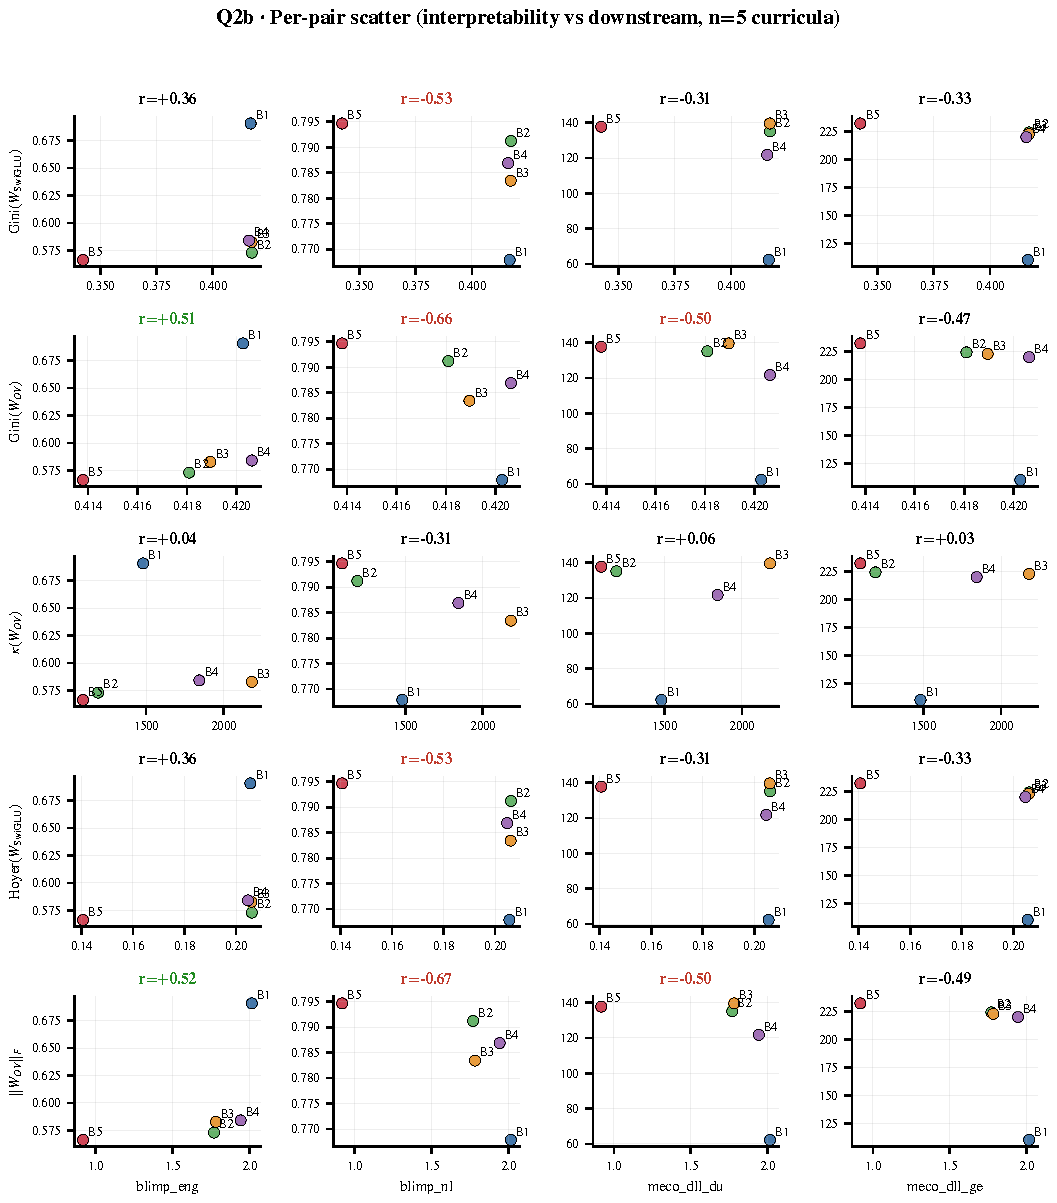
\includegraphics[width=\linewidth]{fig/pico_q2b_scatter_grid.pdf}
  \caption{\textbf{Q2b -- Per-pair scatter.} Scatter for a curated subset of (interpretability metric $\times$ downstream metric) pairs over the $n=5$ nld--eng curricula. Curriculum labels (B1--B5) annotated on each panel; per-panel Pearson $r$ in the title. The B1$\leftrightarrow$B5 separation along $\Vert W_{OV}\Vert_F$ and Gini$(W_{\text{SwiGLU}})$ is visible directly in the per-panel point cloud; treat the regression slopes as exploratory at $n=5$.}
  \label{fig:pico-q2b}
\end{figure}

\begin{figure}[!ht]
  \centering
  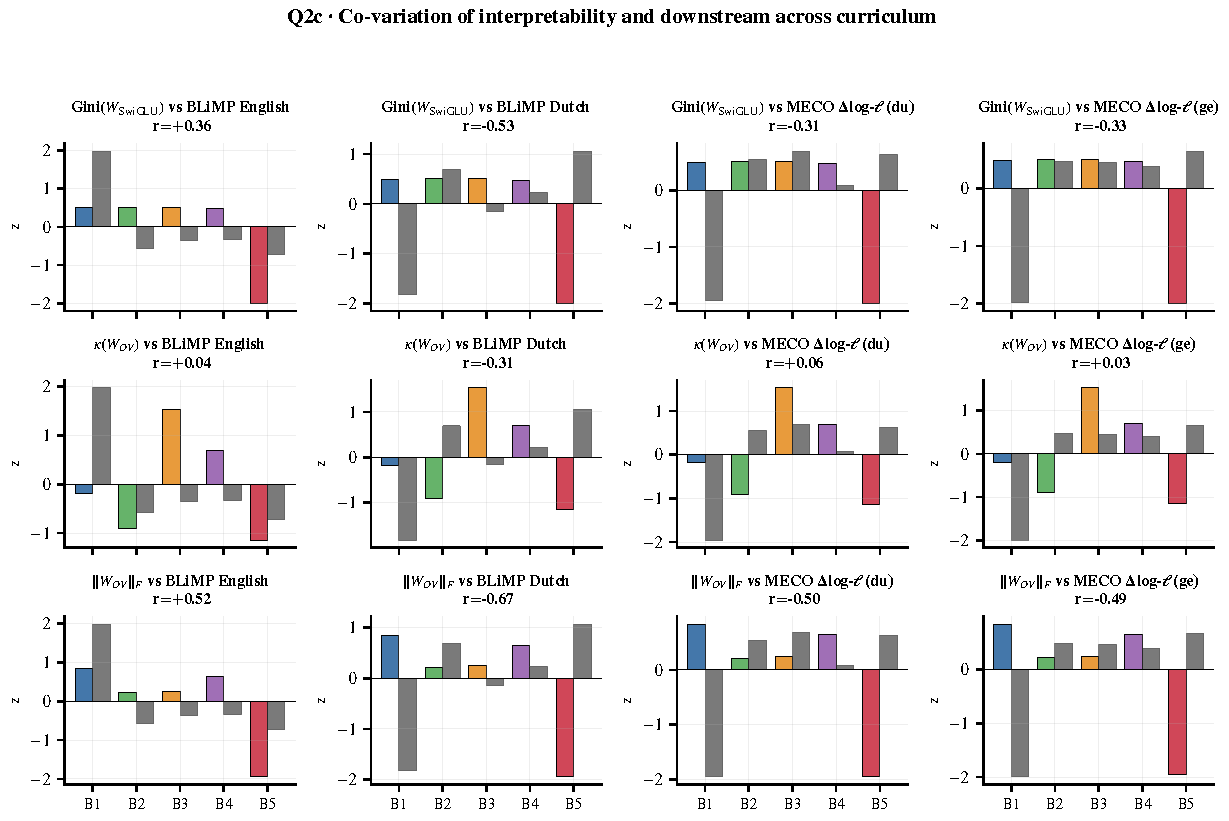
\includegraphics[width=\linewidth]{fig/pico_q2c_paired_bars.pdf}
  \caption{\textbf{Q2c -- Paired $z$-scored bars.} For each curriculum (B1--B5), each interpretability metric is paired with a downstream metric on a common $z$-axis. Co-variation is read as ``same height $\Rightarrow$ same direction''; sign-flip clusters --- e.g.\ $\Vert W_{OV}\Vert_F$ vs.\ BLiMP-nl, Gini$(W_{\text{SwiGLU}})$ vs.\ MECO~du --- visualise the specialisation--generalisation trade-off referenced in \S\ref{sec:interp-comparative} (this is the figure reproduced as Fig.~\ref{fig:pico-q2c-main}).}
  \label{fig:pico-q2c}
\end{figure}

\subsection{Principal correlations and summary}\label{sec:pico-headline}

The principal Q2 results, exact reproductions of the per-pair Pearson $r$ values plotted in Fig.~\ref{fig:pico-q2a} and tabulated in \texttt{ledger\_q2\_joined.csv}, are summarised in Table~\ref{tab:pico-q2-headline}.

\begin{table}[h]
  \centering
  \small
  \caption{Pearson $r$ across the $n=5$ nld--eng curriculum sweep (B1--B5) for selected (interpretability metric, downstream metric) pairs. Bold cells exceed $|r|>0.5$. From \texttt{ledger\_q2\_joined.csv}.}
  \label{tab:pico-q2-headline}
  \begin{tabular}{lrrrr}
    \toprule
    metric & BLiMP-eng & BLiMP-nl & MECO-du & MECO-ge \\
    \midrule
    $\Vert W_{OV}\Vert_F$       & \textbf{+0.52} & \textbf{$-$0.67} & $-$0.50 & $-$0.49 \\
    Gini$(W_{\text{SwiGLU}})$   & $+$0.36        & \textbf{$-$0.53} & $-$0.31 & $-$0.33 \\
    Hoyer$(W_{\text{SwiGLU}})$  & $+$0.36        & \textbf{$-$0.53} & $-$0.37 & $-$0.33 \\
    $\Vert W_{\text{norm}}\Vert_F$ & $-$0.44     & \textbf{$+$0.60} & \textbf{$+$0.54} & $+$0.42 \\
    $\kappa(W_{OV})$            & $+$0.04        & $-$0.31          & $+$0.06 & $+$0.03 \\
    \bottomrule
  \end{tabular}
\end{table}

\paragraph{Take-home.} The interpretability metrics in \textsc{Pico-Analyze} do not measure a single latent ``model quality'' axis. They measure \emph{specialisation vs.\ generalisation}: high Gini/Hoyer/Frobenius on the OV+SwiGLU subspaces buy English BLiMP at the cost of L1 transfer and psycholinguistic alignment. The curriculum that maximises BLiMP-eng (B1, balanced 50/50) and the curriculum that maximises L1 retention and human-RT alignment (B5, late l2-80) lie at opposite ends of the same axis the interpretability metrics are sensitive to.

\paragraph{Caveats.} (i) $n=5$ for every Q2 correlation; treat $r$-values as exploratory; bootstrap CIs over the curriculum sweep are pending. (ii) Downstream evaluations are at \textsc{HumanScale} (0.1~B token); interpretability metrics are at \textsc{FineWeb}-100M ($\sim$0.1~B token). Same parameter count and effective token budget, but the corpora differ; a matched-corpus re-run (interpretability on \textsc{HumanScale} checkpoints) would tighten the join. (iii) \textsc{BLiSS} excluded as noted above. (iv) \textsc{Pico} run \texttt{beetle-bilingual-balanced-b1-fineweb-100m-rus-eng} contributes to Q1 only.

\section{Detailed Results}


\begin{figure}[!htbp]
  \centering
  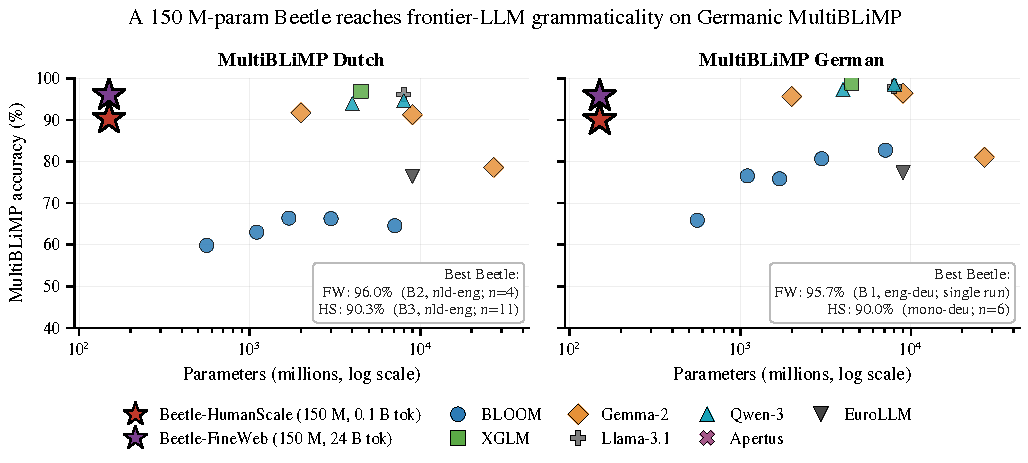
\includegraphics[width=0.86\linewidth,height=0.78\textheight,keepaspectratio]{fig/F1_multiblimp_pareto_baselines.pdf}
  \caption{MultiBLiMP Pareto frontier: per-language grammaticality accuracy for \textsc{Beetle} bilingual curricula B1--B5 (\textsc{HumanScale}~100M and \textsc{FineWeb}~2B token budgets) against the BLOOM 560M--7B1 ladder, XGLM-4.5B, EuroLLM-9B, Apertus-8B, Gemma-2-9B, and Qwen-3 baselines. Reproduced at full resolution from main-body Fig.~\ref{fig:multiblimp_pareto}.}
  \label{appcomp:F1_multiblimp_pareto_baselines}
\end{figure}

\begin{figure}[!htbp]
  \centering
  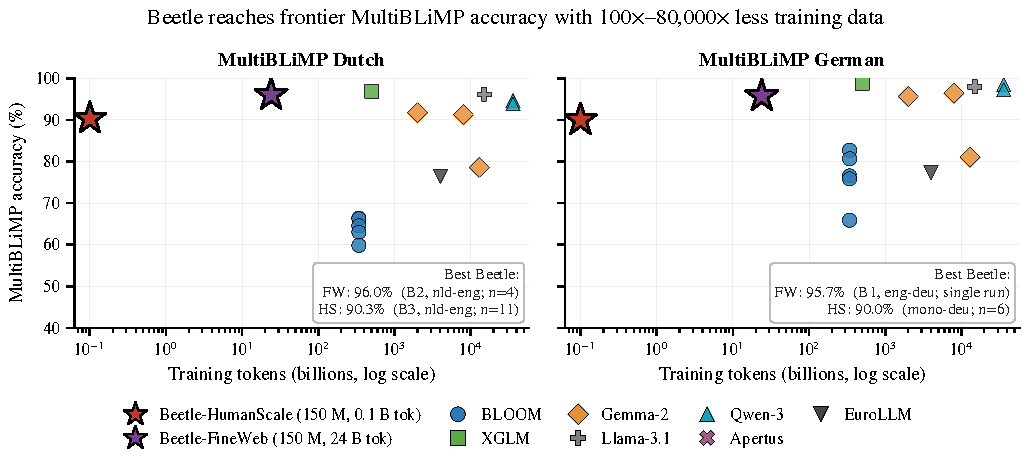
\includegraphics[width=0.86\linewidth,height=0.78\textheight,keepaspectratio]{fig/F2_multiblimp_token_efficiency.pdf}
  \caption{MultiBLiMP Dutch grammaticality accuracy as a function of training tokens (log scale) for \textsc{Beetle} curricula B1--B5 nld--eng compared to the BLOOM ladder and XGLM-4.5B. Reproduced from main-body Fig.~\ref{fig:multiblimp_efficiency}.}
  \label{appcomp:F2_multiblimp_token_efficiency}
\end{figure}

\begin{figure}[!htbp]
  \centering
  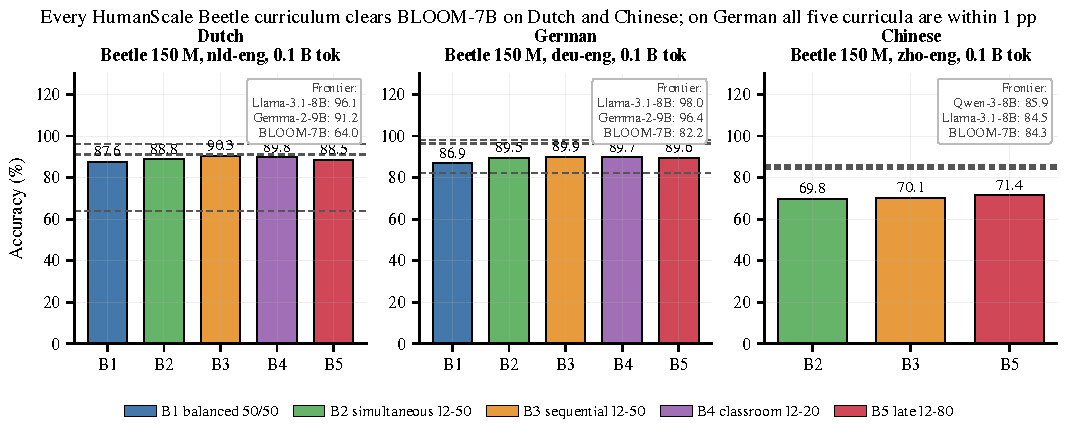
\includegraphics[width=0.86\linewidth,height=0.78\textheight,keepaspectratio]{fig/F3_curriculum_multiblimp.pdf}
  \caption{MultiBLiMP grammaticality accuracy by curriculum (B1--B5) across five target languages (Dutch, German, French, Persian, Bulgarian) for \textsc{Beetle} bilingual nld--eng models at the \textsc{FineWeb}~2B token budget. Reproduced from main-body Fig.~\ref{fig:multiblimp_curriculum}.}
  \label{appcomp:F3_curriculum_multiblimp}
\end{figure}

\begin{figure}[!htbp]
  \centering
  \includegraphics[width=0.86\linewidth,height=0.78\textheight,keepaspectratio]{fig/F4_curriculum_meco_deltaLL.pdf}
  \caption{MECO~L2 $\Delta\log L$ by exposure curriculum (B1--B5) for Dutch, German, and Chinese L2 reader groups, evaluated on the matched MECO~L2 split. The cross-curriculum ordering is the inverse of the MultiBLiMP ordering shown in Fig.~\ref{appcomp:F3_curriculum_multiblimp}; reproduced from main-body Fig.~\ref{fig:meco_curriculum}.}
  \label{appcomp:F4_curriculum_meco_deltaLL}
\end{figure}

\begin{figure}[!htbp]
  \centering
  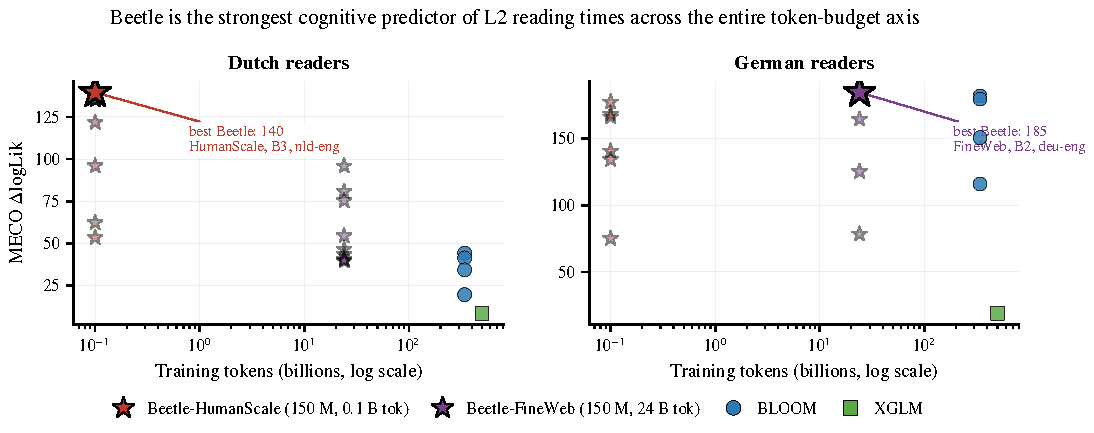
\includegraphics[width=0.86\linewidth,height=0.78\textheight,keepaspectratio]{fig/F5_meco_token_efficiency.pdf}
  \caption{MECO~L2 $\Delta\log L$ as a function of training tokens (log scale) for \textsc{Beetle} curricula B1--B5 (nld--eng and deu--eng) against the BLOOM ladder and XGLM-4.5B. Reproduced from main-body Fig.~\ref{fig:meco_efficiency}.}
  \label{appcomp:F5_meco_token_efficiency}
\end{figure}

\begin{figure}[!htbp]
  \centering
  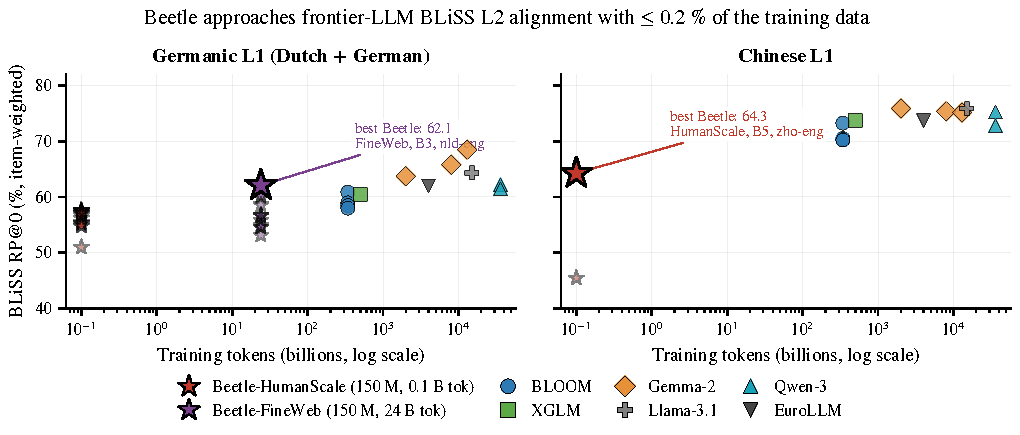
\includegraphics[width=0.86\linewidth,height=0.78\textheight,keepaspectratio]{fig/F6_bliss_token_efficiency.pdf}
  \caption{BLiSS NGS as a function of training tokens for \textsc{Beetle} curricula B1--B5 against the same baselines. Companion to Fig.~\ref{appcomp:F5_meco_token_efficiency}; the curriculum ordering is the inverse of the MECO~L2 ordering.}
  \label{appcomp:F6_bliss_token_efficiency}
\end{figure}

\begin{figure}[!htbp]
  \centering
  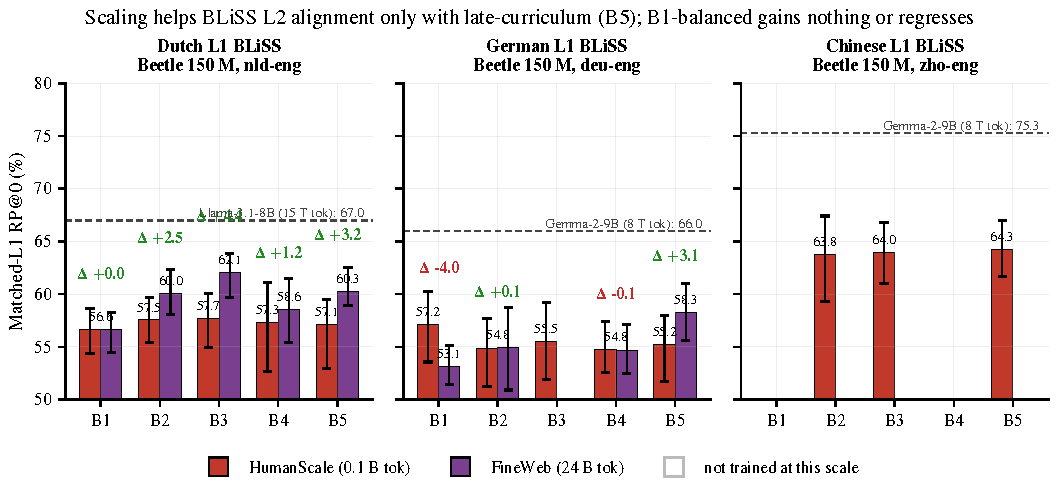
\includegraphics[width=0.86\linewidth,height=0.78\textheight,keepaspectratio]{fig/F7_bliss_curriculum_x_scale.pdf}
  \caption{BLiSS NGS by exposure curriculum $\times$ training scale (\textsc{HumanScale}~100M and \textsc{FineWeb}~2B). Reproduced from main-body Fig.~\ref{fig:bliss_curriculum_scale}.}
  \label{appcomp:F7_bliss_curriculum_x_scale}
\end{figure}

\begin{figure}[!htbp]
  \centering
  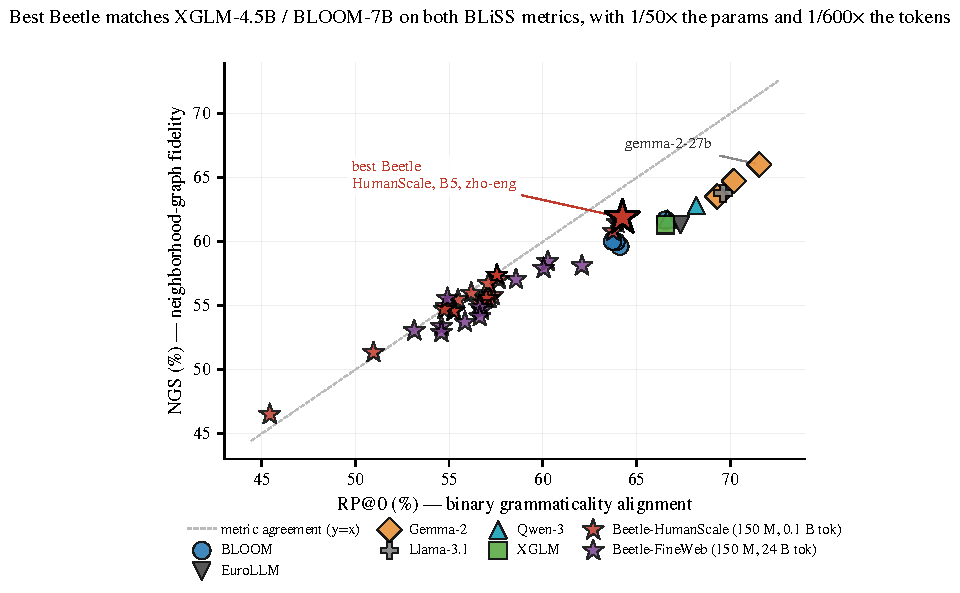
\includegraphics[width=0.86\linewidth,height=0.78\textheight,keepaspectratio]{fig/F8_bliss_metric_tradeoff_pareto.pdf}
  \caption{BLiSS metric trade-off Pareto frontier (NGS, CPS, RP$@\tau$) across \textsc{Beetle} curricula and the baseline cohort. Reproduced from main-body Fig.~\ref{fig:bliss_pareto}.}
  \label{appcomp:F8_bliss_metric_tradeoff_pareto}
\end{figure}

\begin{figure}[!htbp]
  \centering
  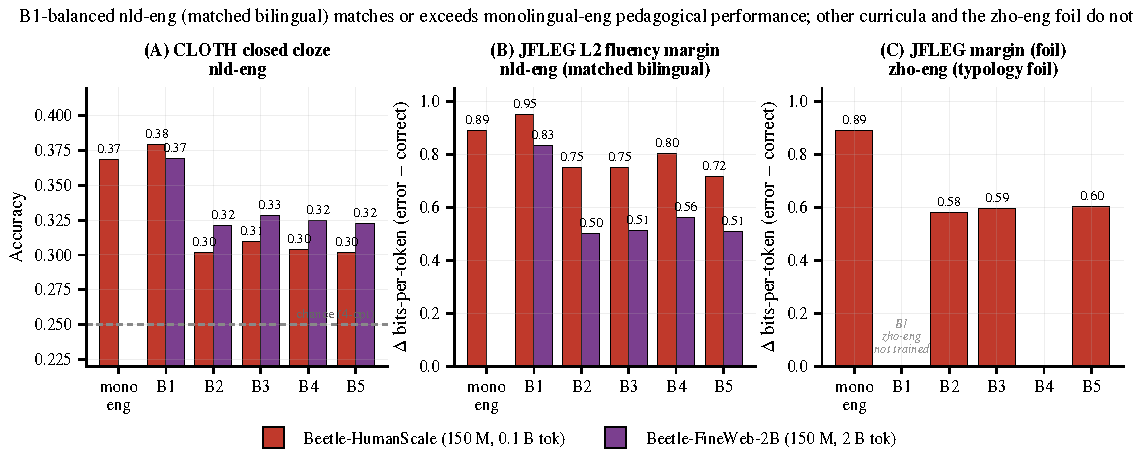
\includegraphics[width=0.86\linewidth,height=0.78\textheight,keepaspectratio]{fig/F9_pedagogical_headline.pdf}
  \caption{Pedagogical evaluation: CLOTH closed-cloze accuracy and JFLEG L2-fluency margin (matched nld--eng; zho--eng foil) by curriculum and training scale. Reproduced from main-body Fig.~\ref{fig:pedagogical_headline}.}
  \label{appcomp:F9_pedagogical_headline}
\end{figure}

\begin{figure}[!htbp]
  \centering
  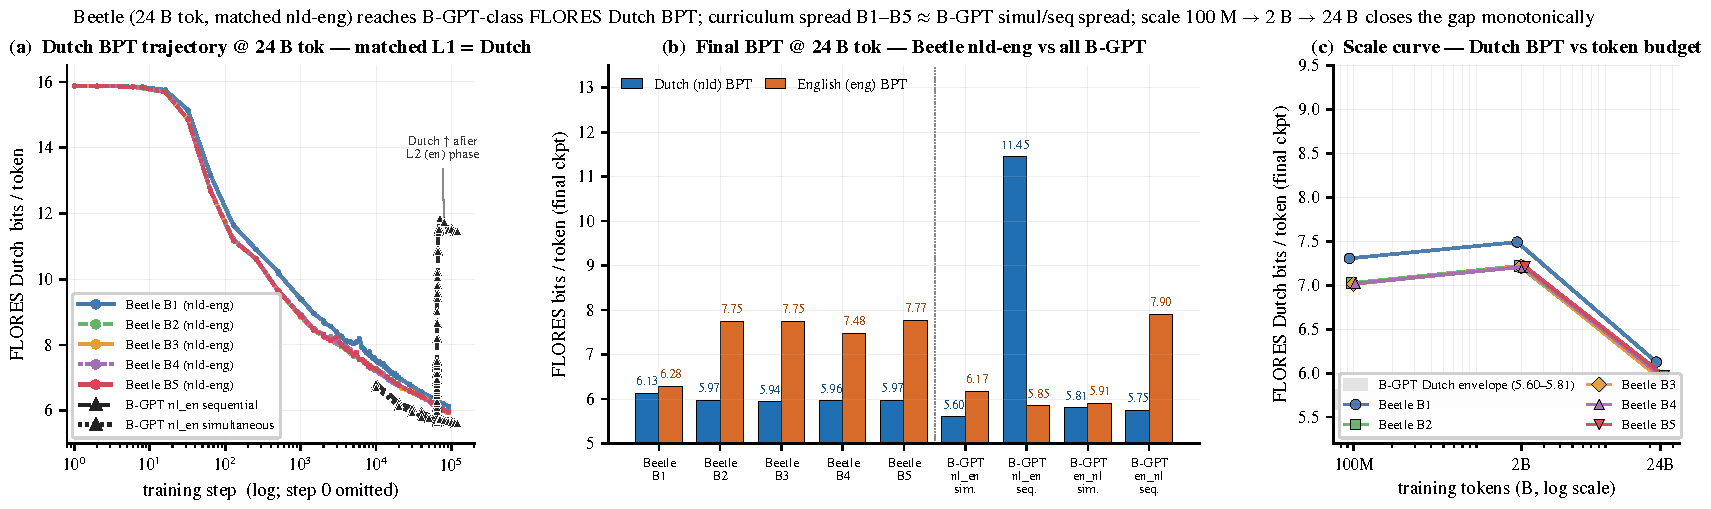
\includegraphics[width=0.86\linewidth,height=0.78\textheight,keepaspectratio]{fig/F10_flores_beetle_vs_bgpt.pdf}
  \caption{FLORES bits-per-byte for matched nld--eng \textsc{Beetle} curricula against B-GPT \citep{arnett-etal-2025-acquisition}: developmental trajectory, final paired bars, and 100M/2B/24B scale curve. Reproduced from main-body Fig.~\ref{fig:flores_beetle_vs_bgpt}.}
  \label{appcomp:F10_flores_beetle_vs_bgpt}
\end{figure}


\section{Detailed MECO}


\begin{figure}[!htbp]
  \centering
  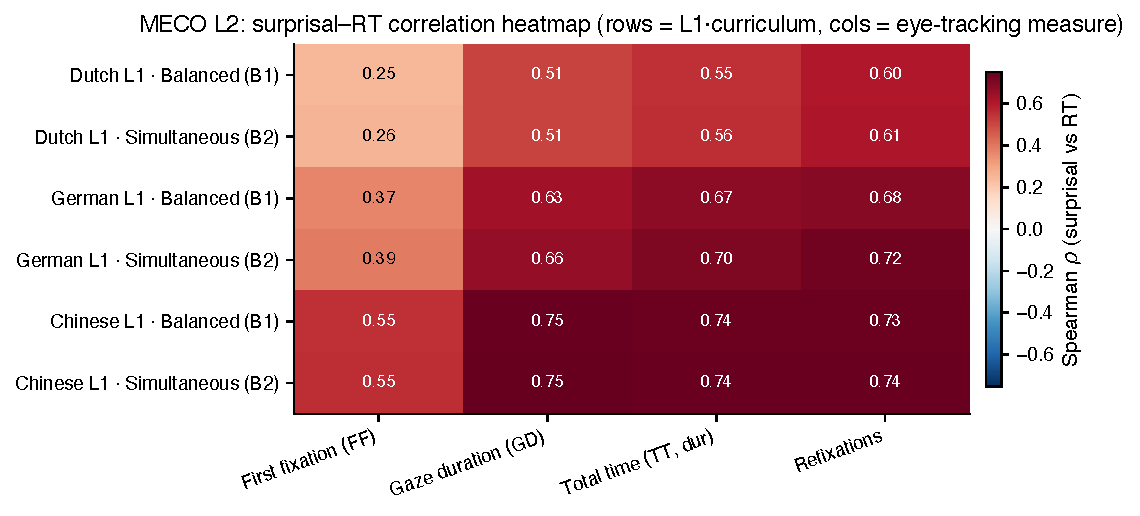
\includegraphics[width=0.86\linewidth,height=0.78\textheight,keepaspectratio]{fig/fig_meco_l2_participants_heatmap.pdf}
  \caption{Per-participant MECO~L2 $\Delta\log L$ heatmap (participant $\times$ model).}
  \label{appcomp:fig_meco_l2_participants_heatmap}
\end{figure}

\newpage
\section{Detailed BLiSS}

\begin{figure}[!htbp]
  \centering
  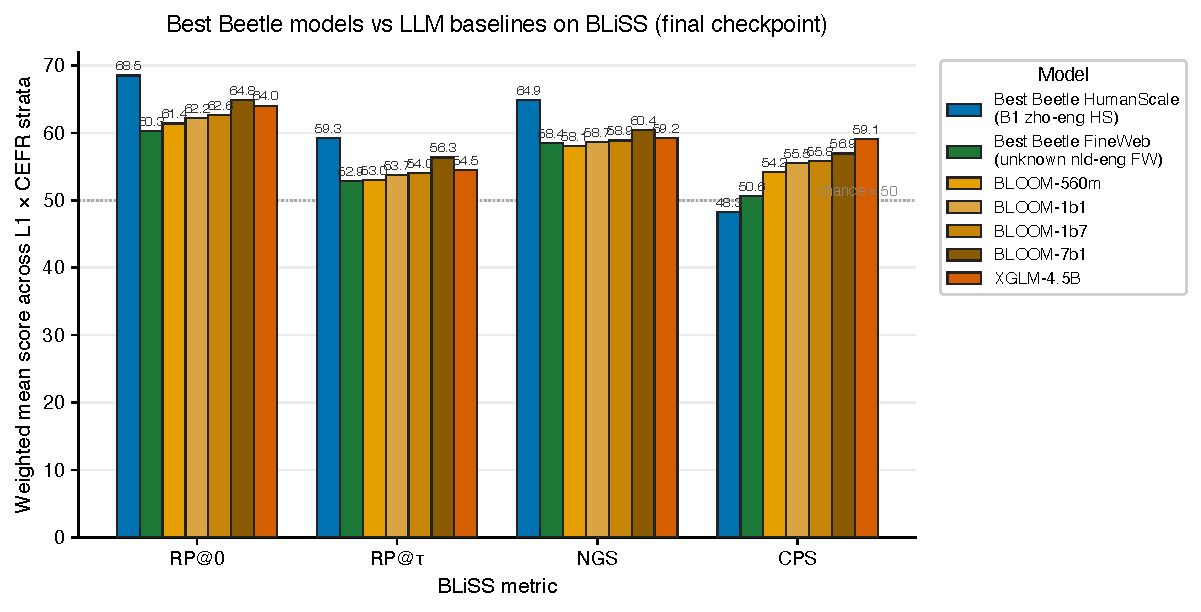
\includegraphics[width=0.86\linewidth,height=0.78\textheight,keepaspectratio]{fig/fig_best_bliss_vs_baselines.pdf}
  \caption{Best \textsc{Beetle} BLiSS NGS (B5 nld--eng \textsc{FineWeb}~2B) against the baseline cohort. Reproduced from main-body Fig.~\ref{fig:bliss_best}.}
  \label{appcomp:fig_best_bliss_vs_baselines}
\end{figure}

\begin{figure}[!htbp]
  \centering
  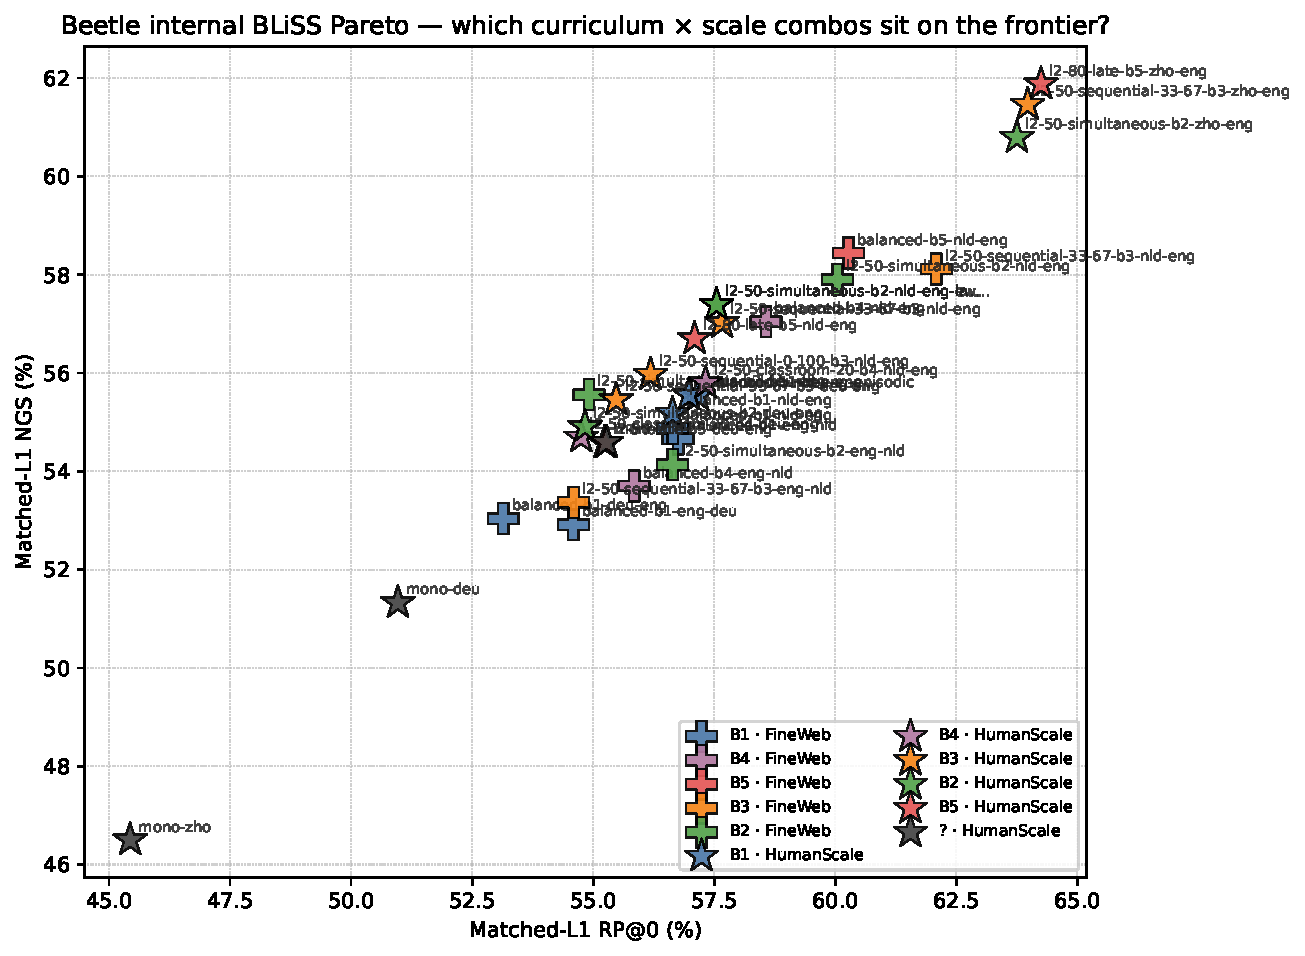
\includegraphics[width=0.86\linewidth,height=0.78\textheight,keepaspectratio]{fig/fig_bliss_beetle_curriculum_frontier.pdf}
  \caption{BLiSS curriculum frontier: NGS as a function of curriculum (B1--B5) at the \textsc{FineWeb}~2B token budget.}
  \label{appcomp:fig_bliss_beetle_curriculum_frontier}
\end{figure}

\begin{figure}[!htbp]
  \centering
  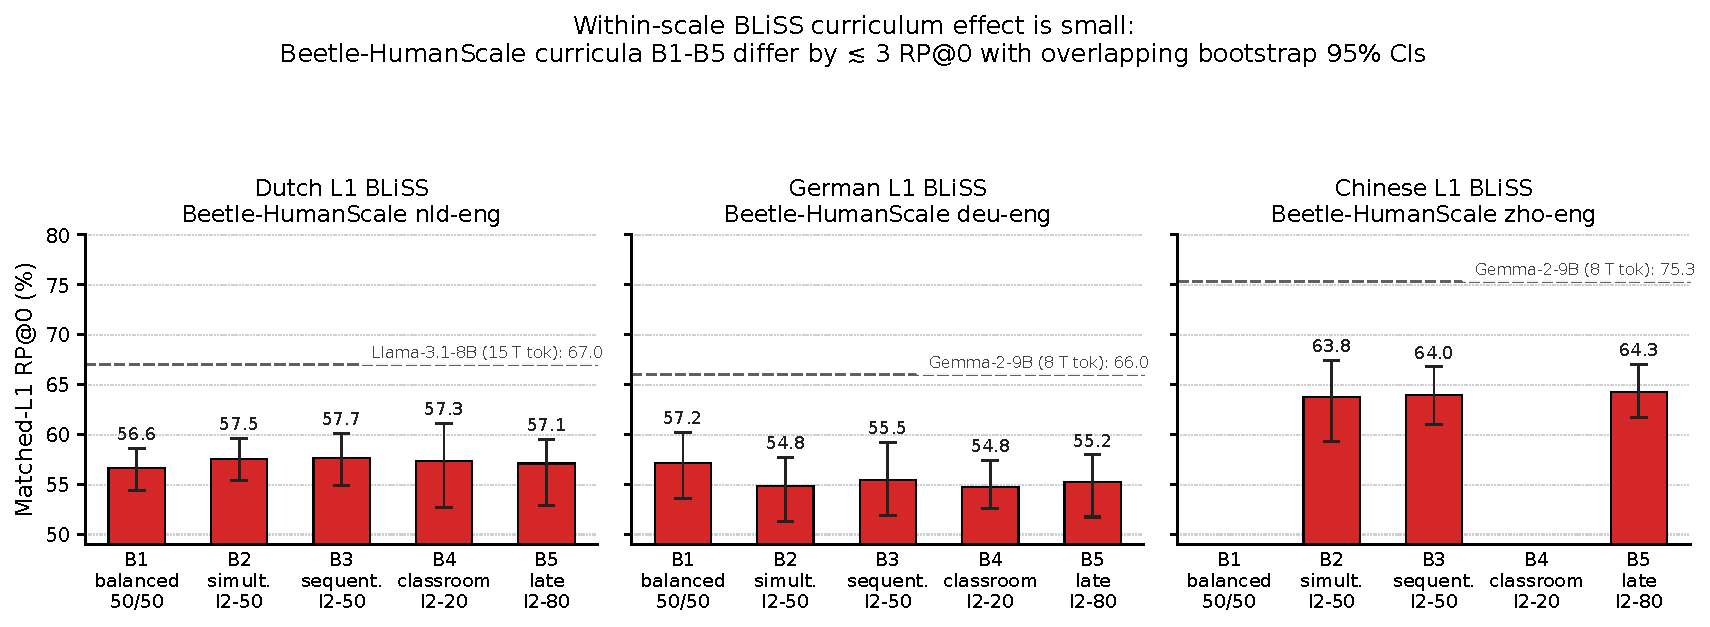
\includegraphics[width=0.86\linewidth,height=0.78\textheight,keepaspectratio]{fig/fig_bliss_curriculum_supp.pdf}
  \caption{Supplementary BLiSS curriculum diagnostics on CPS and RP$@\tau$.}
  \label{appcomp:fig_bliss_curriculum_supp}
\end{figure}

\begin{figure}[!htbp]
  \centering
  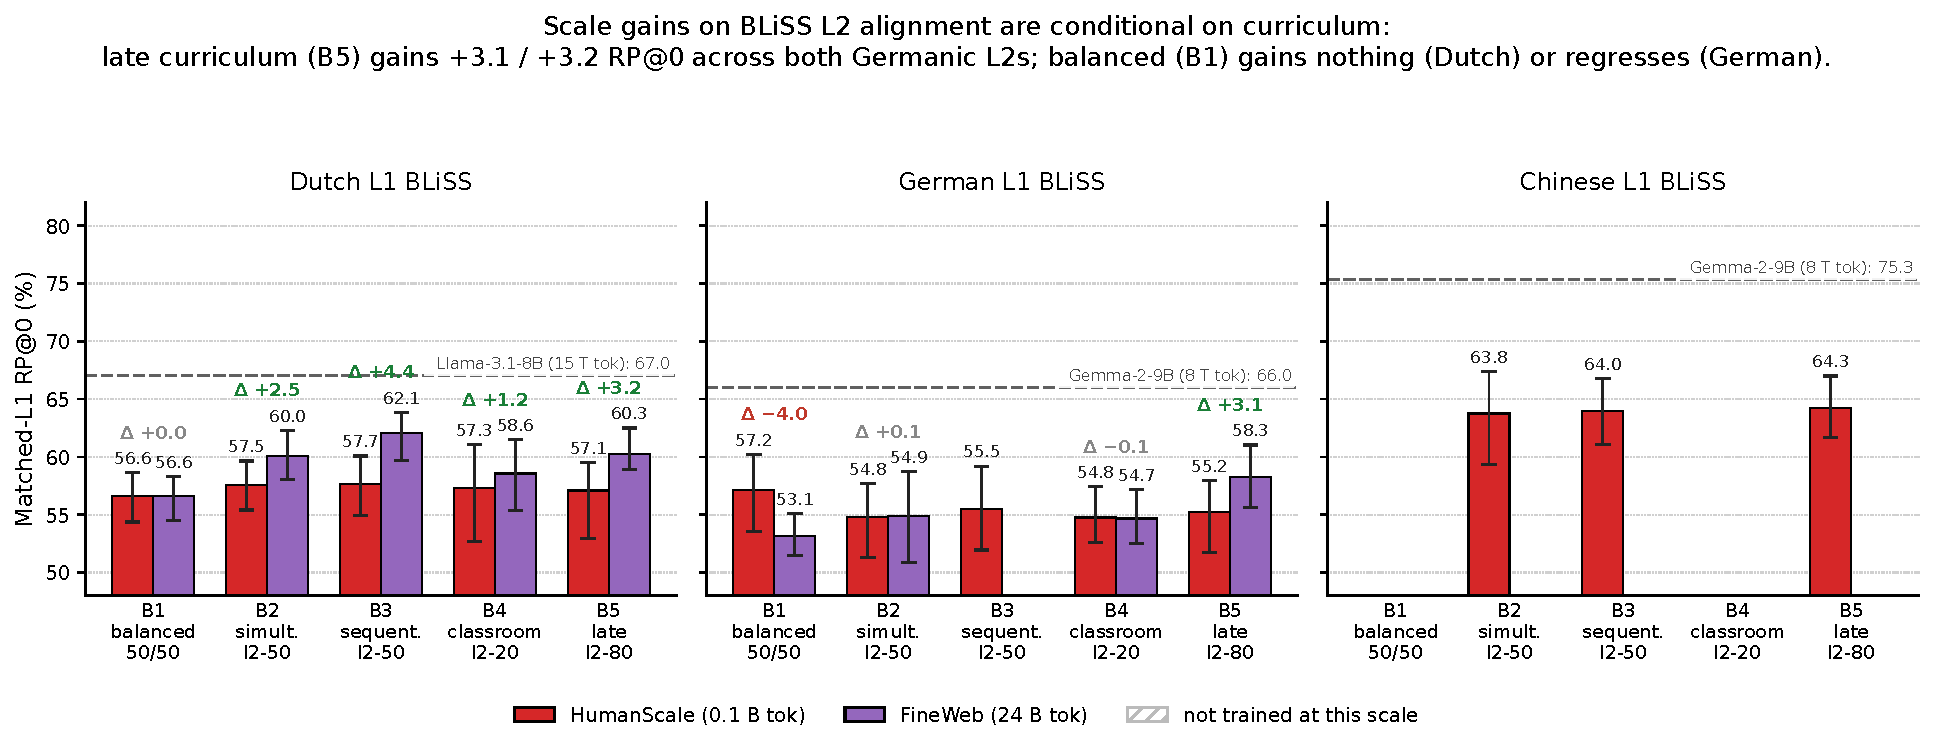
\includegraphics[width=0.86\linewidth,height=0.78\textheight,keepaspectratio]{fig/fig_bliss_main_curriculum.pdf}
  \caption{Aggregated BLiSS NGS by curriculum across all \textsc{Beetle} L1 cohorts.}
  \label{appcomp:fig_bliss_main_curriculum}
\end{figure}

\begin{figure}[!htbp]
  \centering
  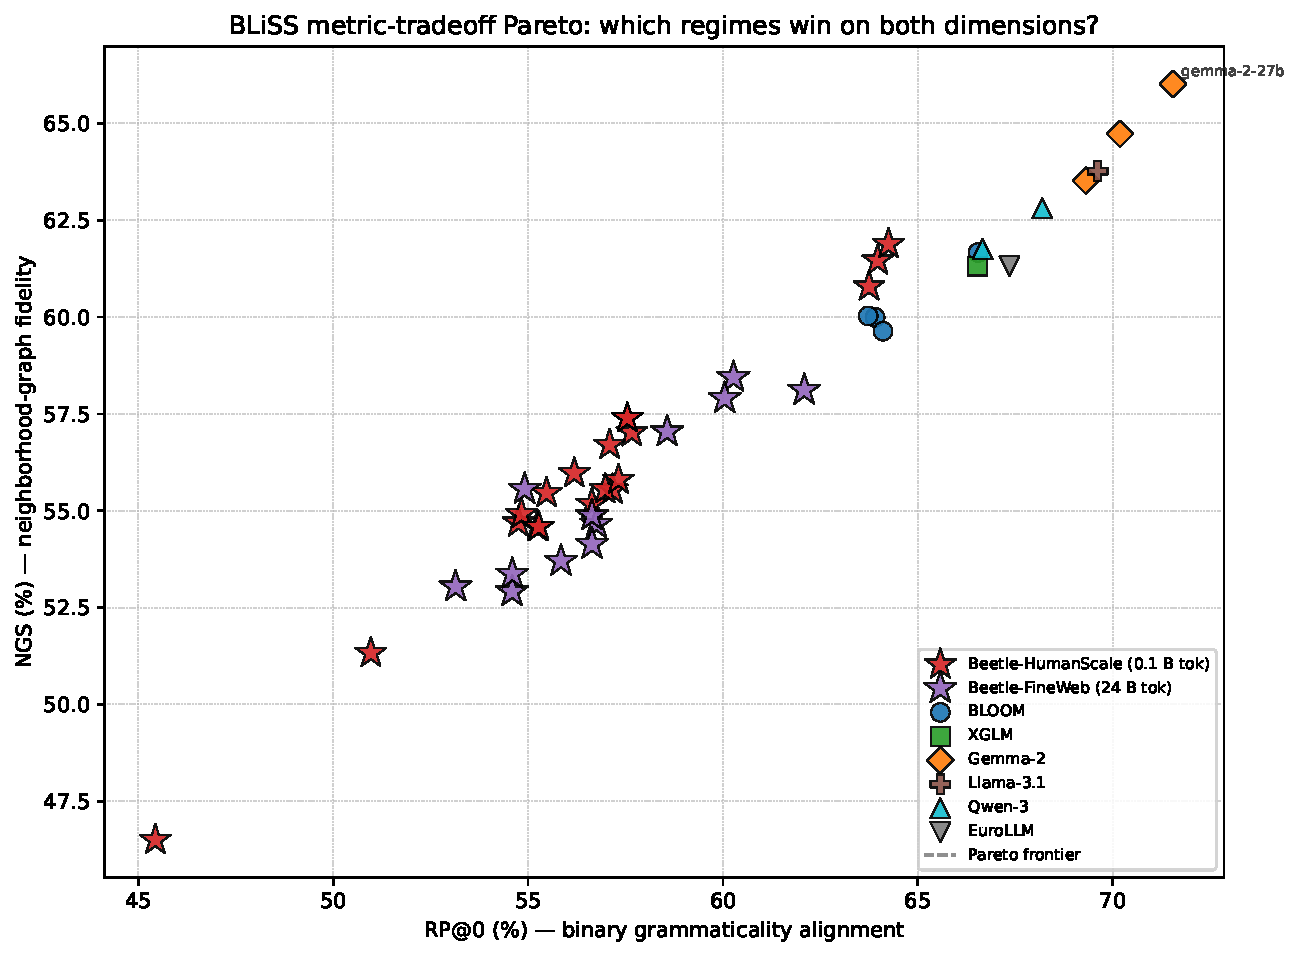
\includegraphics[width=0.86\linewidth,height=0.78\textheight,keepaspectratio]{fig/fig_bliss_pareto_metric_tradeoff.pdf}
  \caption{BLiSS Pareto metric trade-off (NGS, CPS, RP$@\tau$); companion to Fig.~\ref{appcomp:F8_bliss_metric_tradeoff_pareto}.}
  \label{appcomp:fig_bliss_pareto_metric_tradeoff}
\end{figure}

\begin{figure}[!htbp]
  \centering
  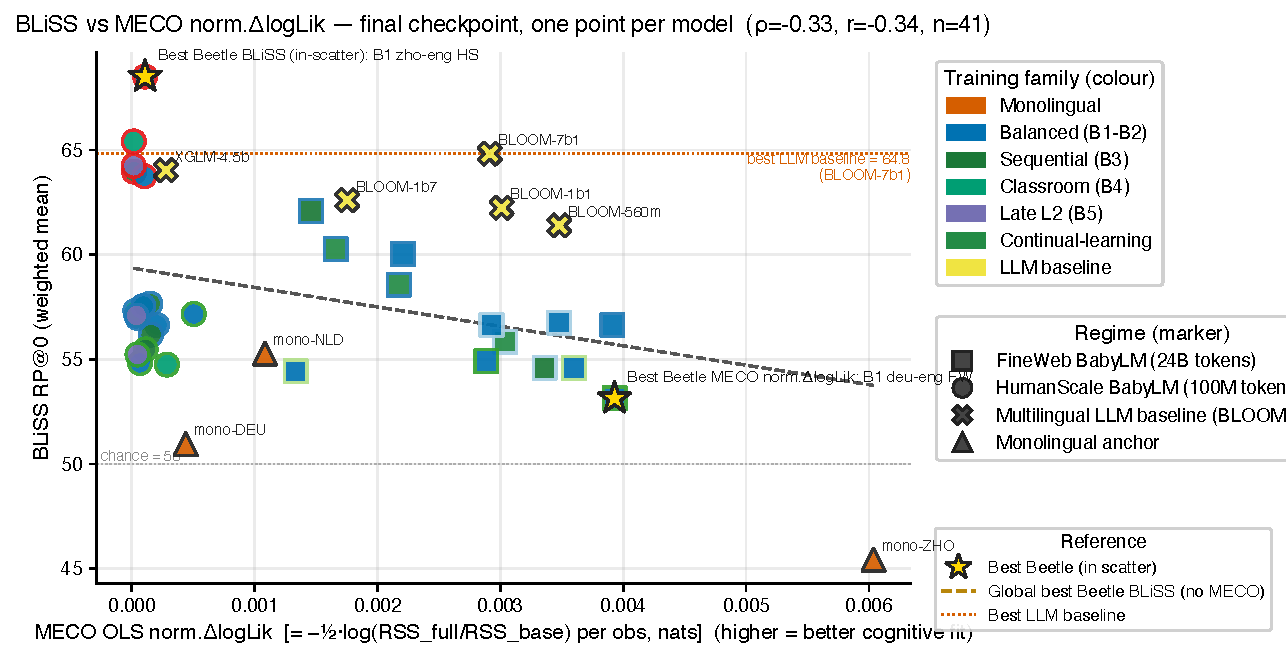
\includegraphics[width=0.86\linewidth,height=0.78\textheight,keepaspectratio]{fig/fig_bliss_vs_meco_final.pdf}
  \caption{Final-checkpoint scatter of BLiSS NGS against MECO~L2 $\Delta\log L$ coloured by curriculum: the Pareto-inversion visualisation underlying \S\ref{sec:results}.}
  \label{appcomp:fig_bliss_vs_meco_final}
\end{figure}

\newpage 
\section{Detailed Pedagogical Tasks}


\begin{figure}[!htbp]
  \centering
  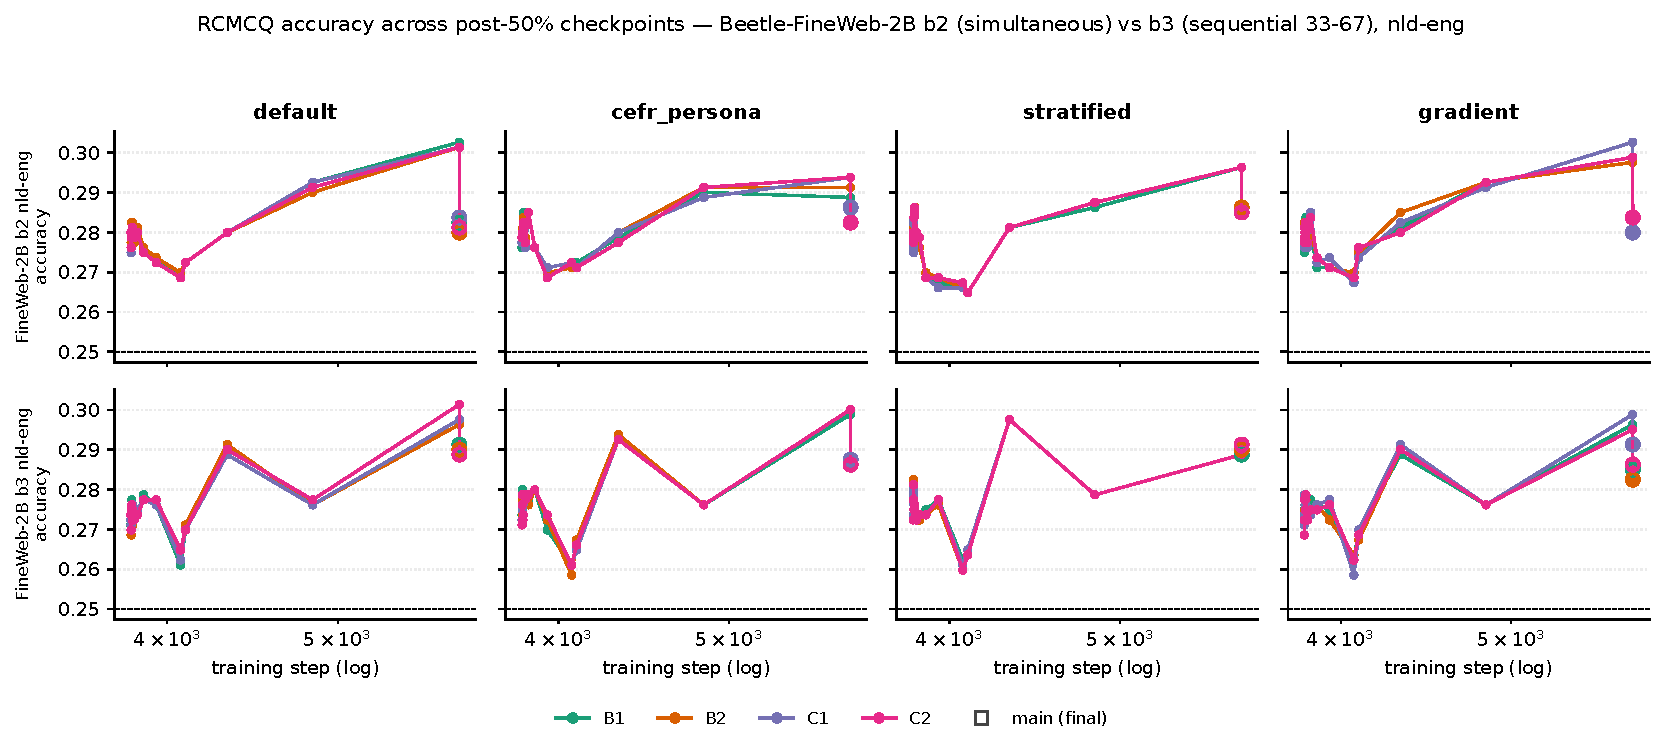
\includegraphics[width=0.86\linewidth,height=0.78\textheight,keepaspectratio]{fig/figC_ckpt_rcmcq_trace.pdf}
  \caption{Reading-comprehension multiple-choice accuracy trace across log-spaced 24B-token \textsc{Beetle} checkpoints.}
  \label{appcomp:figC_ckpt_rcmcq_trace}
\end{figure}

\begin{figure}[!htbp]
  \centering
  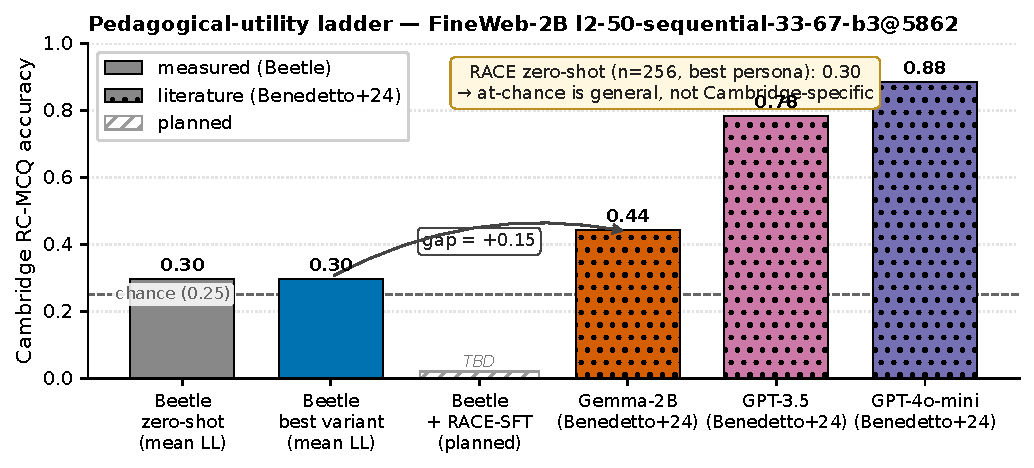
\includegraphics[width=0.86\linewidth,height=0.78\textheight,keepaspectratio]{fig/figC_pedagogical_utility.pdf}
  \caption{Composite pedagogical-utility figure across the CUP\&A5, CLOTH, JFLEG, and EVP evaluation axes.}
  \label{appcomp:figC_pedagogical_utility}
\end{figure}

\begin{figure}[!htbp]
  \centering
  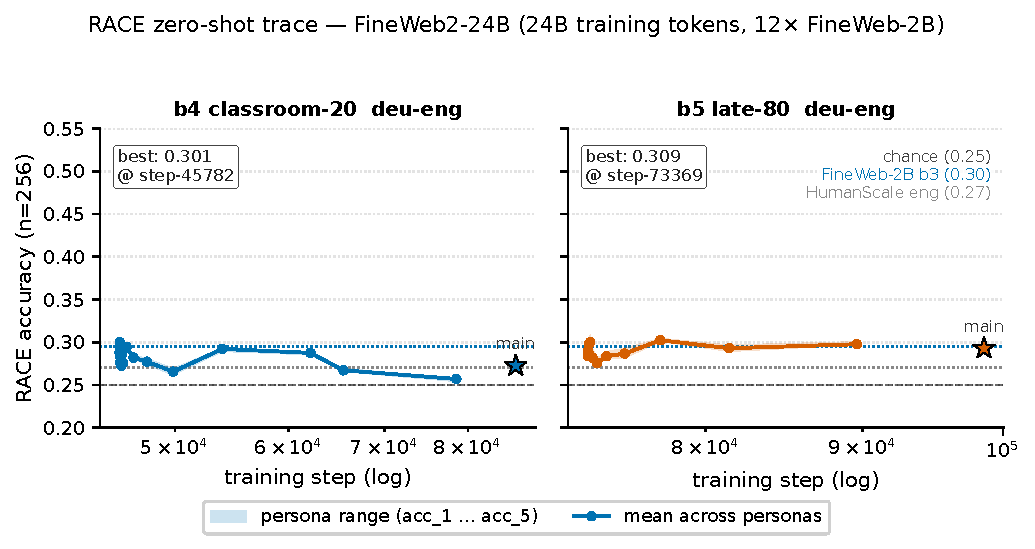
\includegraphics[width=0.86\linewidth,height=0.78\textheight,keepaspectratio]{fig/figC_race_24b_trace.pdf}
  \caption{RACE zero-shot accuracy trace across 24B-token \textsc{Beetle} checkpoints (pre-fine-tuning baseline).}
  \label{appcomp:figC_race_24b_trace}
\end{figure}

\begin{figure}[!htbp]
  \centering
  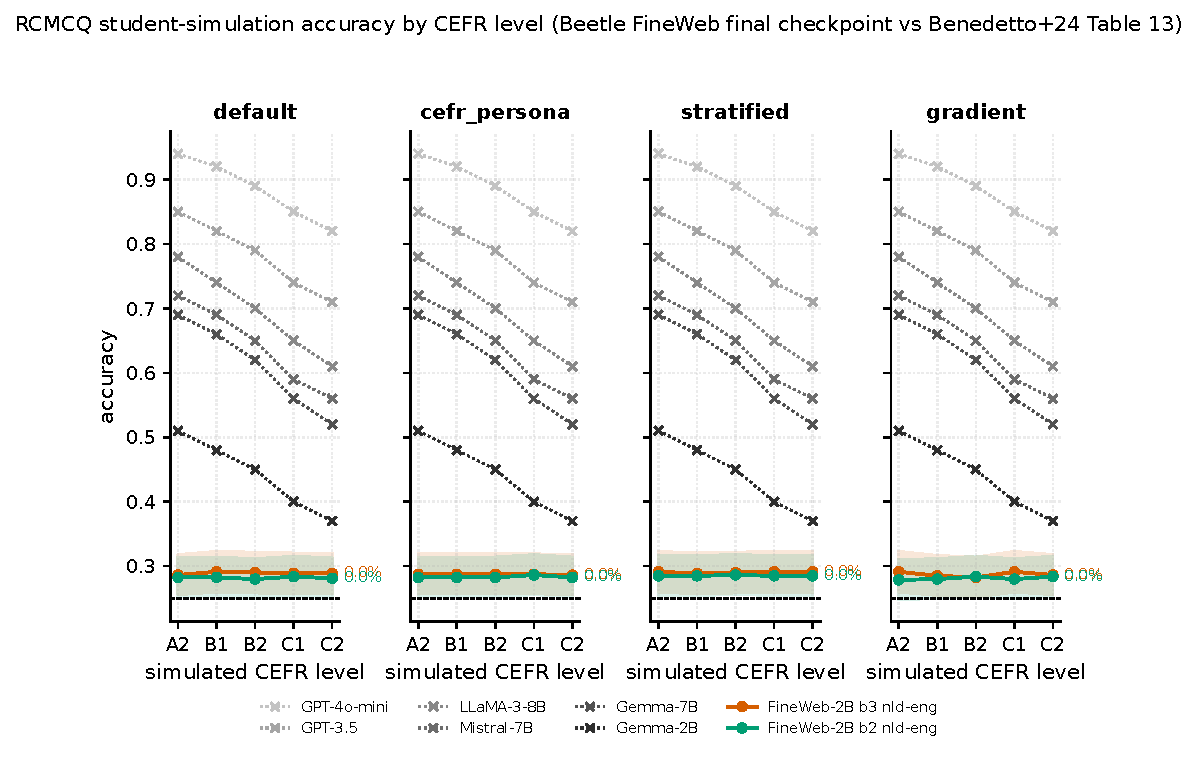
\includegraphics[width=0.86\linewidth,height=0.78\textheight,keepaspectratio]{fig/figC_rcmcq_cefr.pdf}
  \caption{CEFR-stratified reading-comprehension multiple-choice accuracy across the four prompting variants of CUP\&A5.}
  \label{appcomp:figC_rcmcq_cefr}
\end{figure}

\begin{figure}[!htbp]
  \centering
  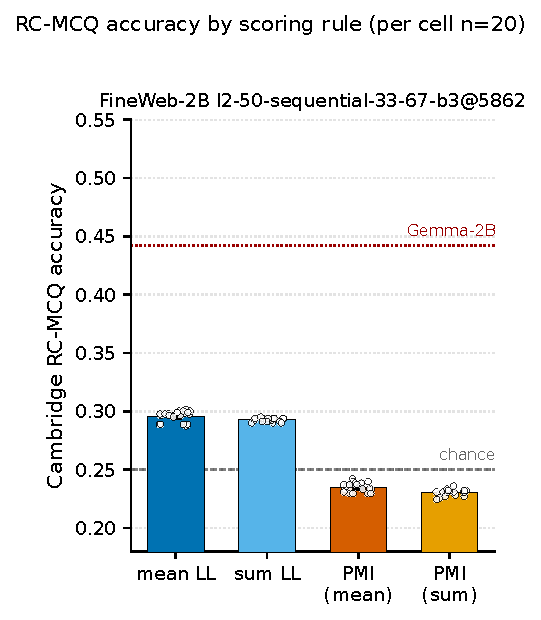
\includegraphics[width=0.86\linewidth,height=0.78\textheight,keepaspectratio]{fig/figC_score_variants.pdf}
  \caption{Score-variant ablation for the CUP\&A5 reading-comprehension task across normalisation choices.}
  \label{appcomp:figC_score_variants}
\end{figure}

\begin{figure}[!htbp]
  \centering
  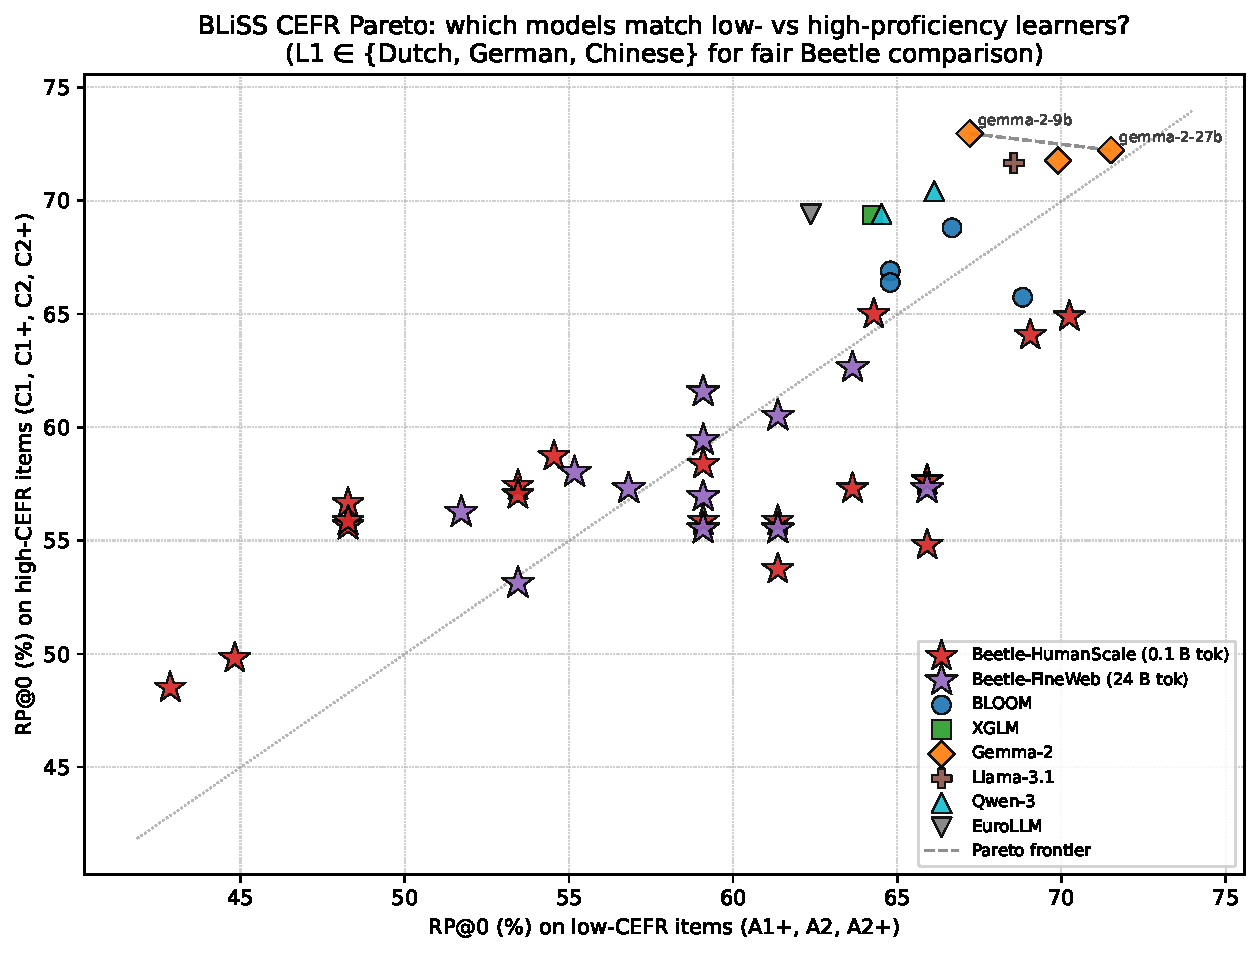
\includegraphics[width=0.86\linewidth,height=0.78\textheight,keepaspectratio]{fig/fig_bliss_pareto_cefr.pdf}
  \caption{BLiSS Pareto frontier cross-referenced against CEFR difficulty stratification.}
  \label{appcomp:fig_bliss_pareto_cefr}
\end{figure}

\begin{figure}[!htbp]
  \centering
  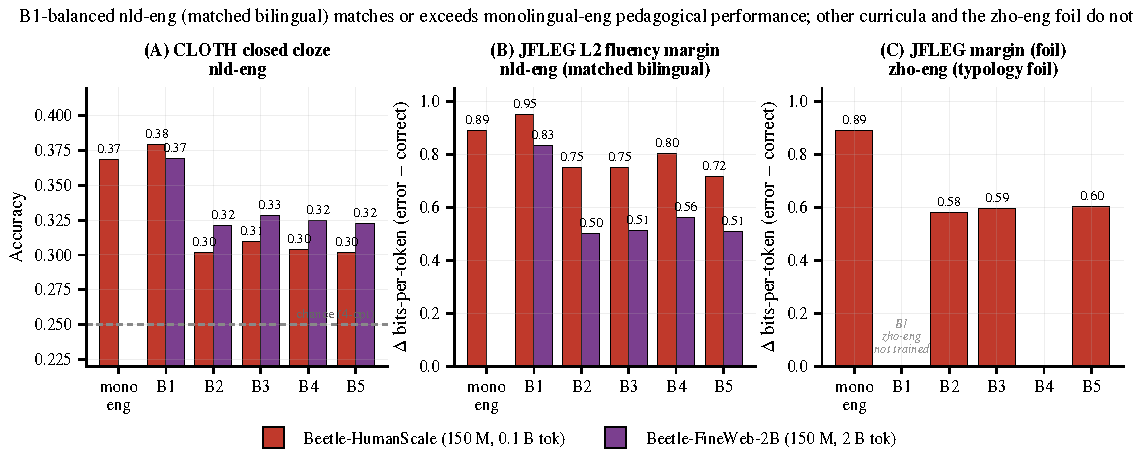
\includegraphics[width=0.86\linewidth,height=0.78\textheight,keepaspectratio]{fig/headline_pedagogical_2x2.pdf}
  \caption{Pedagogical-evidence 2$\times$2 grid: CEFR perplexity gradient, CLOTH closed-cloze accuracy, interlanguage discrimination, and EVP trajectory.}
  \label{appcomp:headline_pedagogical_2x2}
\end{figure}

\begin{figure}[!htbp]
  \centering
  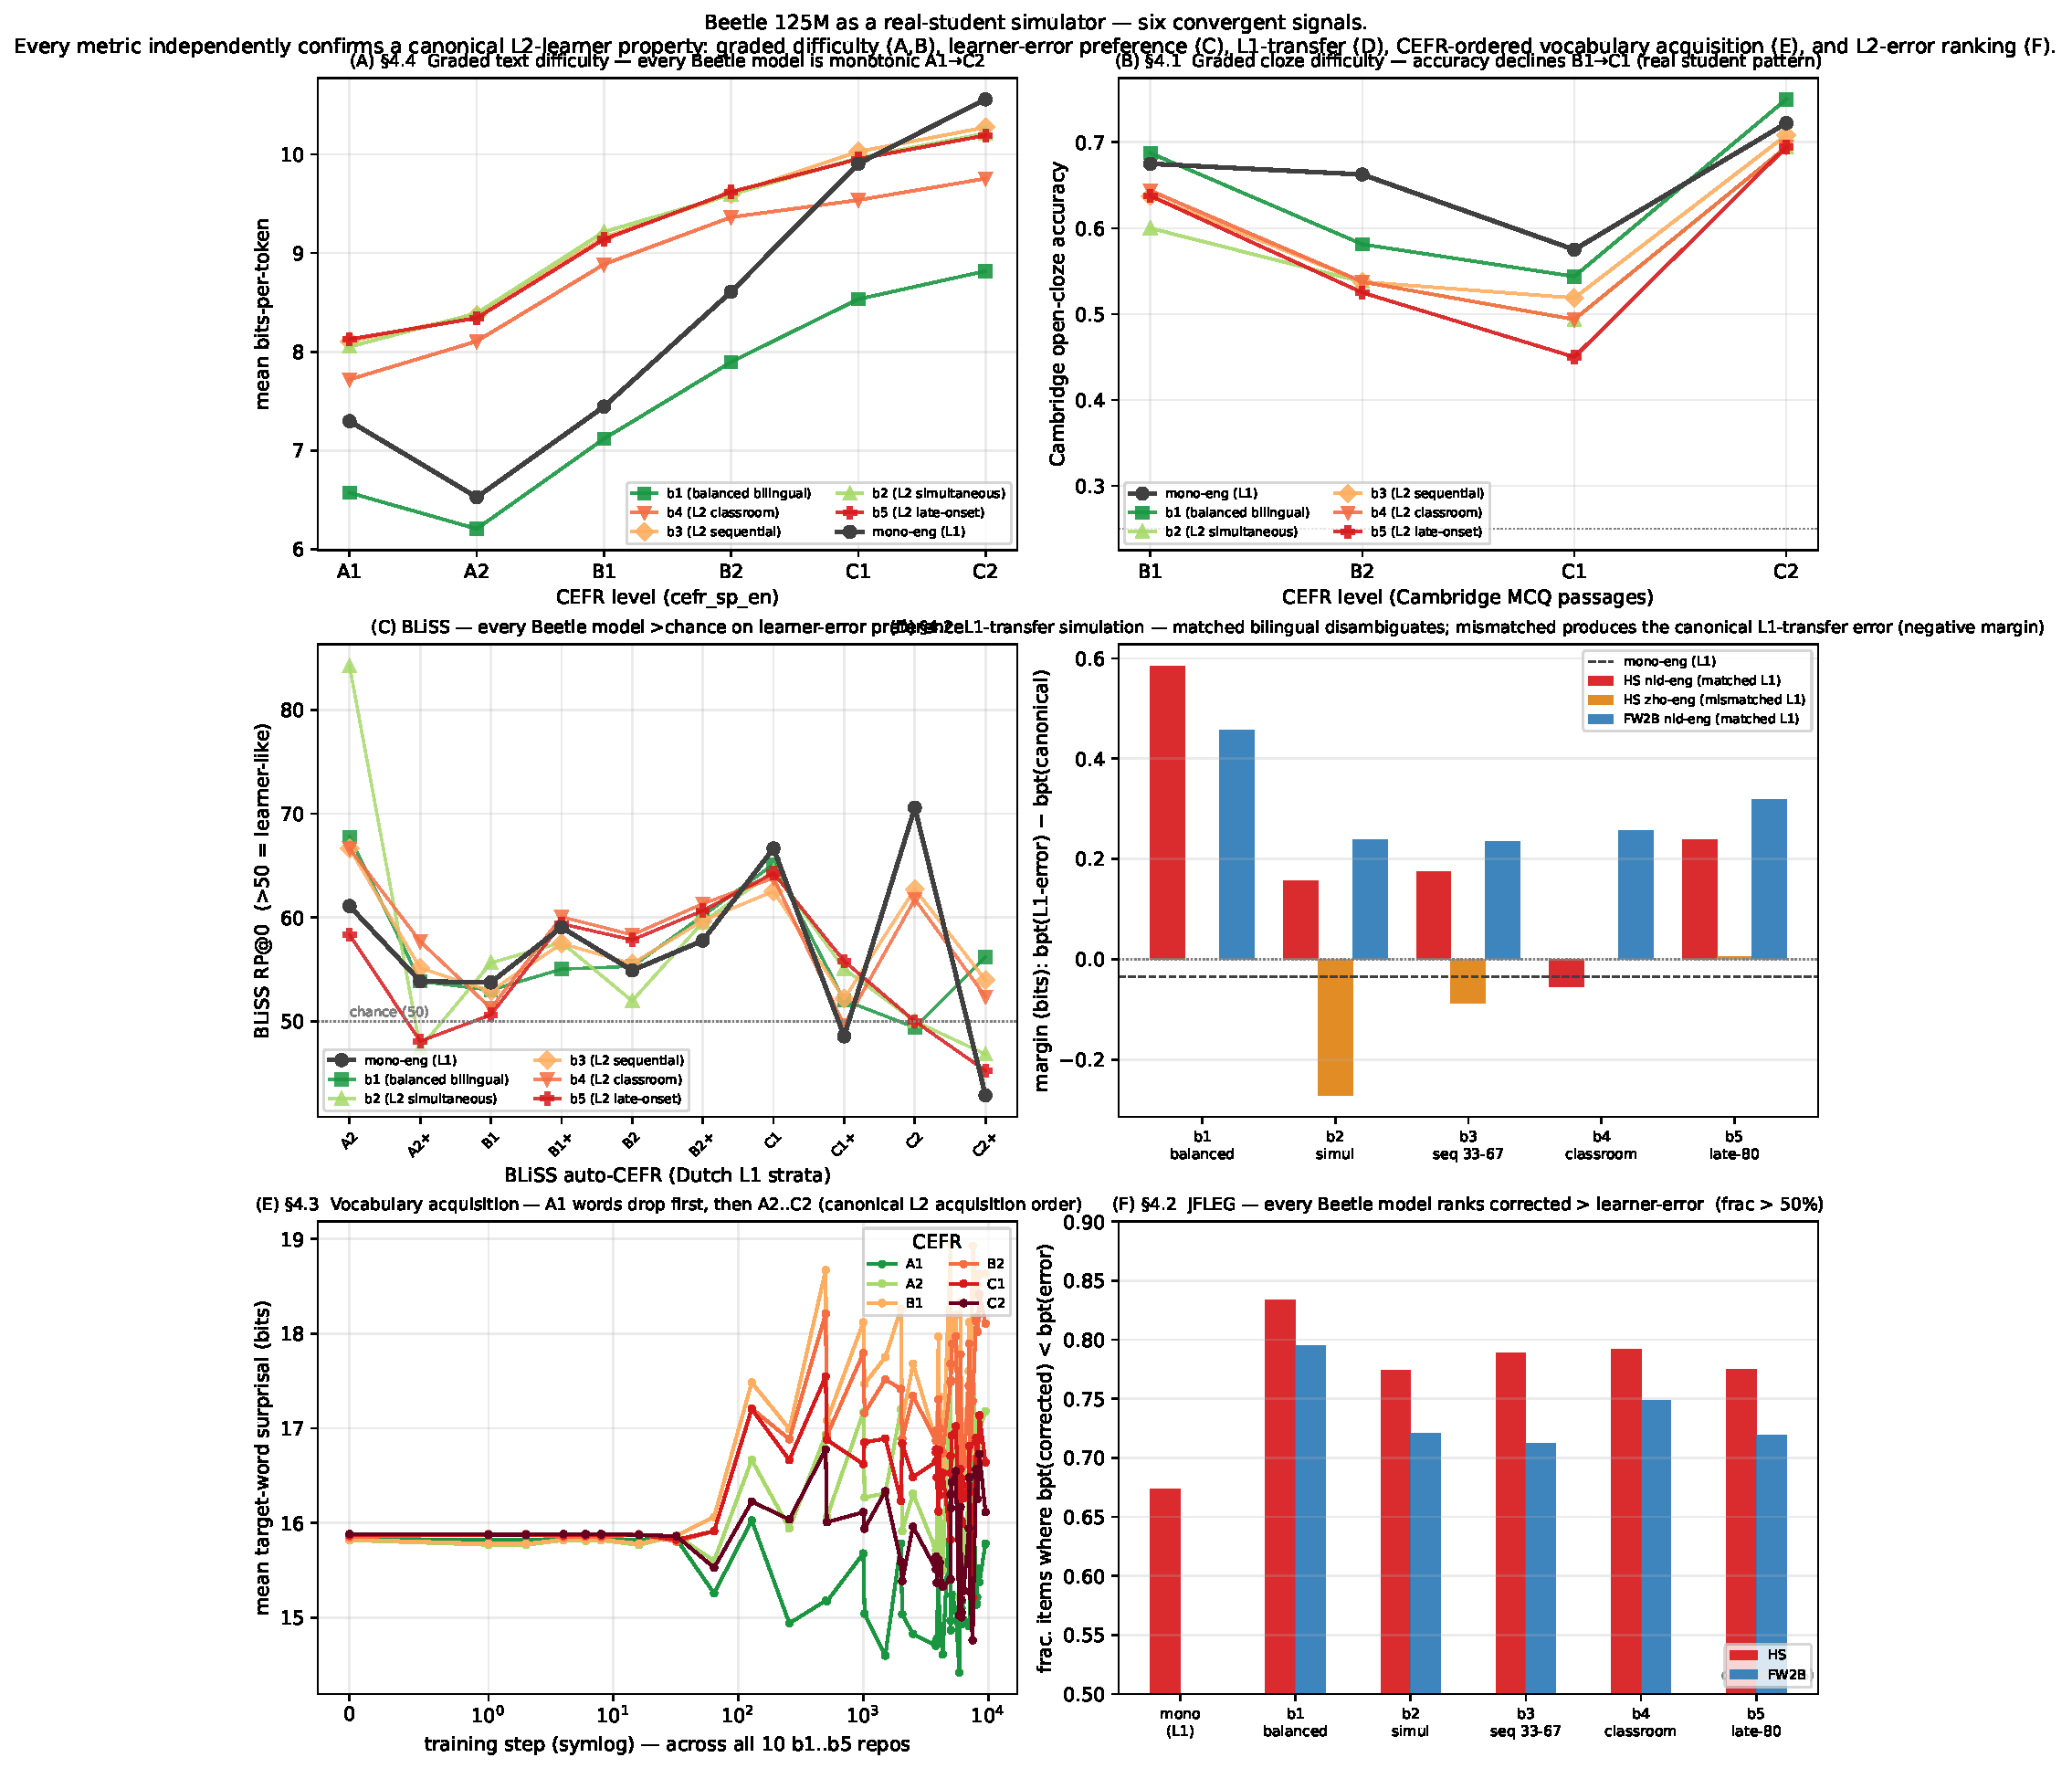
\includegraphics[width=0.86\linewidth,height=0.78\textheight,keepaspectratio]{fig/headline_pedagogical_evidence.pdf}
  \caption{Consolidated pedagogical-evidence panel; companion to main-body Fig.~\ref{fig:pedagogical_headline}.}
  \label{appcomp:headline_pedagogical_evidence}
\end{figure}

\begin{figure}[!htbp]
  \centering
  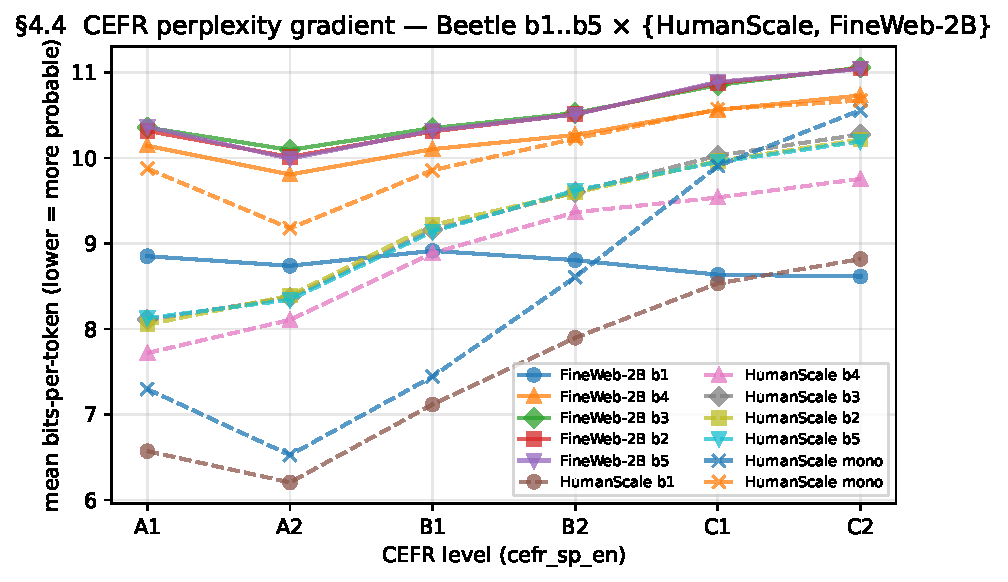
\includegraphics[width=0.86\linewidth,height=0.78\textheight,keepaspectratio]{fig/panelA_cefr_ppl_gradient.pdf}
  \caption{CEFR perplexity gradient (A1--C2) for \textsc{Beetle} curricula and the baseline cohort.}
  \label{appcomp:panelA_cefr_ppl_gradient}
\end{figure}

\begin{figure}[!htbp]
  \centering
  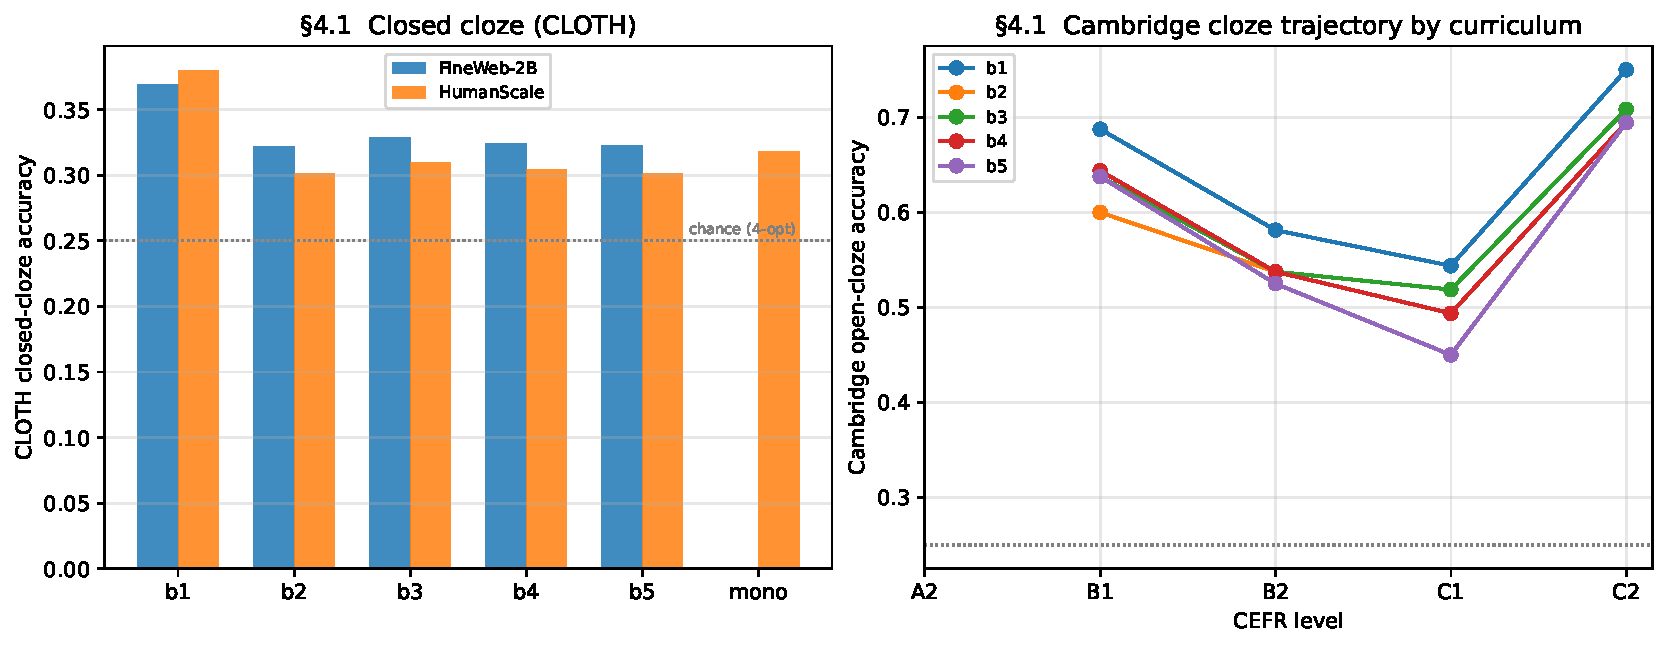
\includegraphics[width=0.86\linewidth,height=0.78\textheight,keepaspectratio]{fig/panelB_cloze.pdf}
  \caption{CLOTH closed-cloze accuracy by CEFR level for \textsc{Beetle} curricula.}
  \label{appcomp:panelB_cloze}
\end{figure}

\begin{figure}[!htbp]
  \centering
  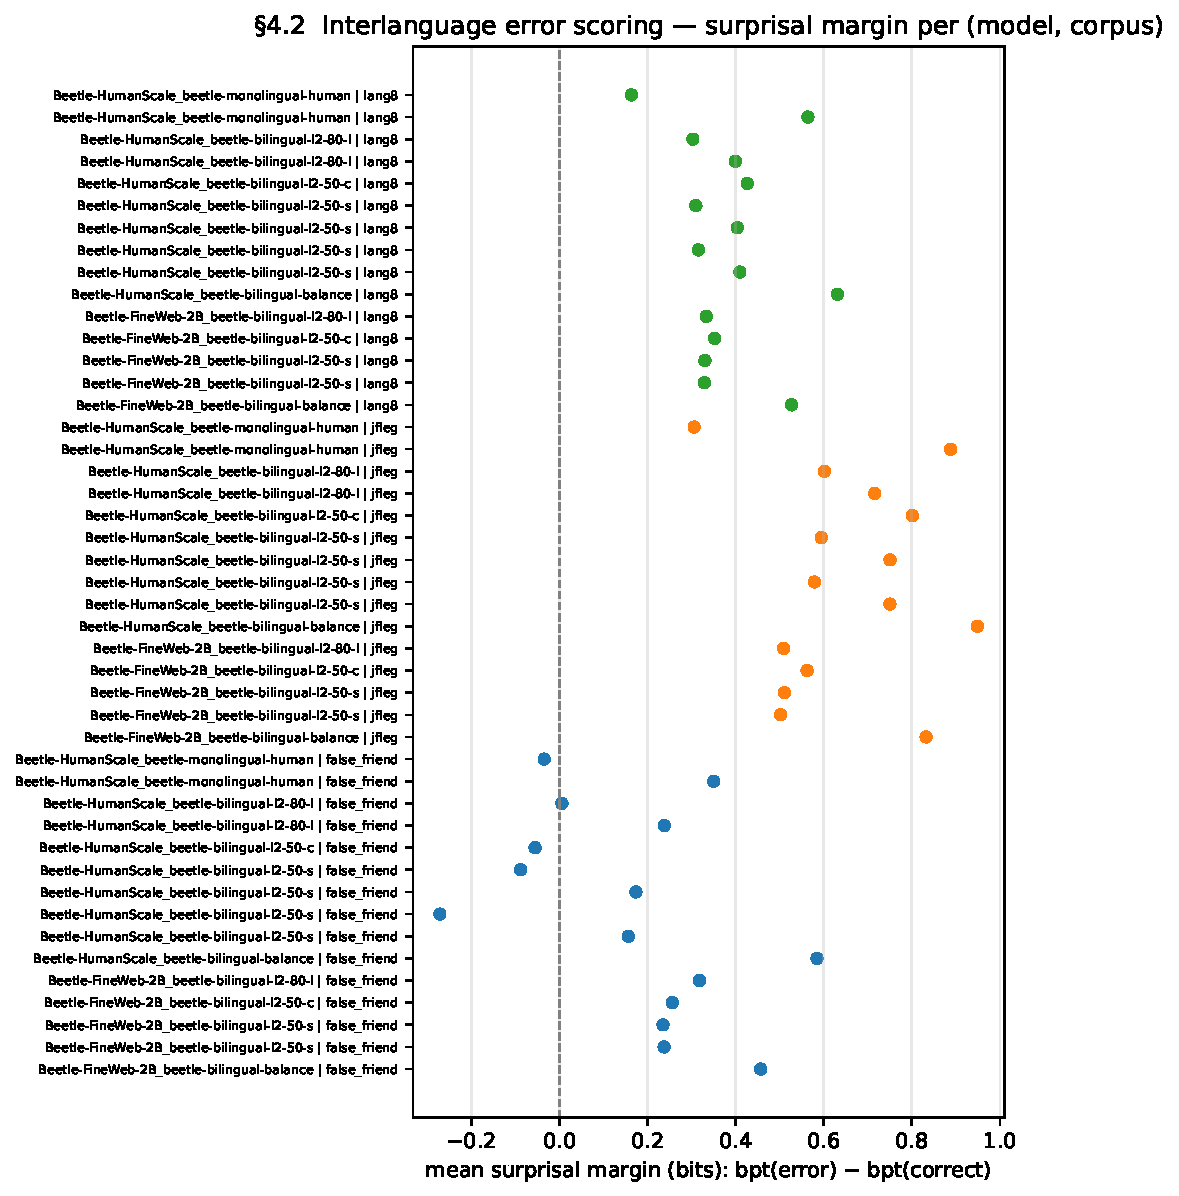
\includegraphics[width=0.86\linewidth,height=0.78\textheight,keepaspectratio]{fig/panelC_interlanguage_forest.pdf}
  \caption{Interlanguage error-discrimination forest plot for the pedagogical evaluation cohort.}
  \label{appcomp:panelC_interlanguage_forest}
\end{figure}


\begin{figure}[!htbp]
  \centering
  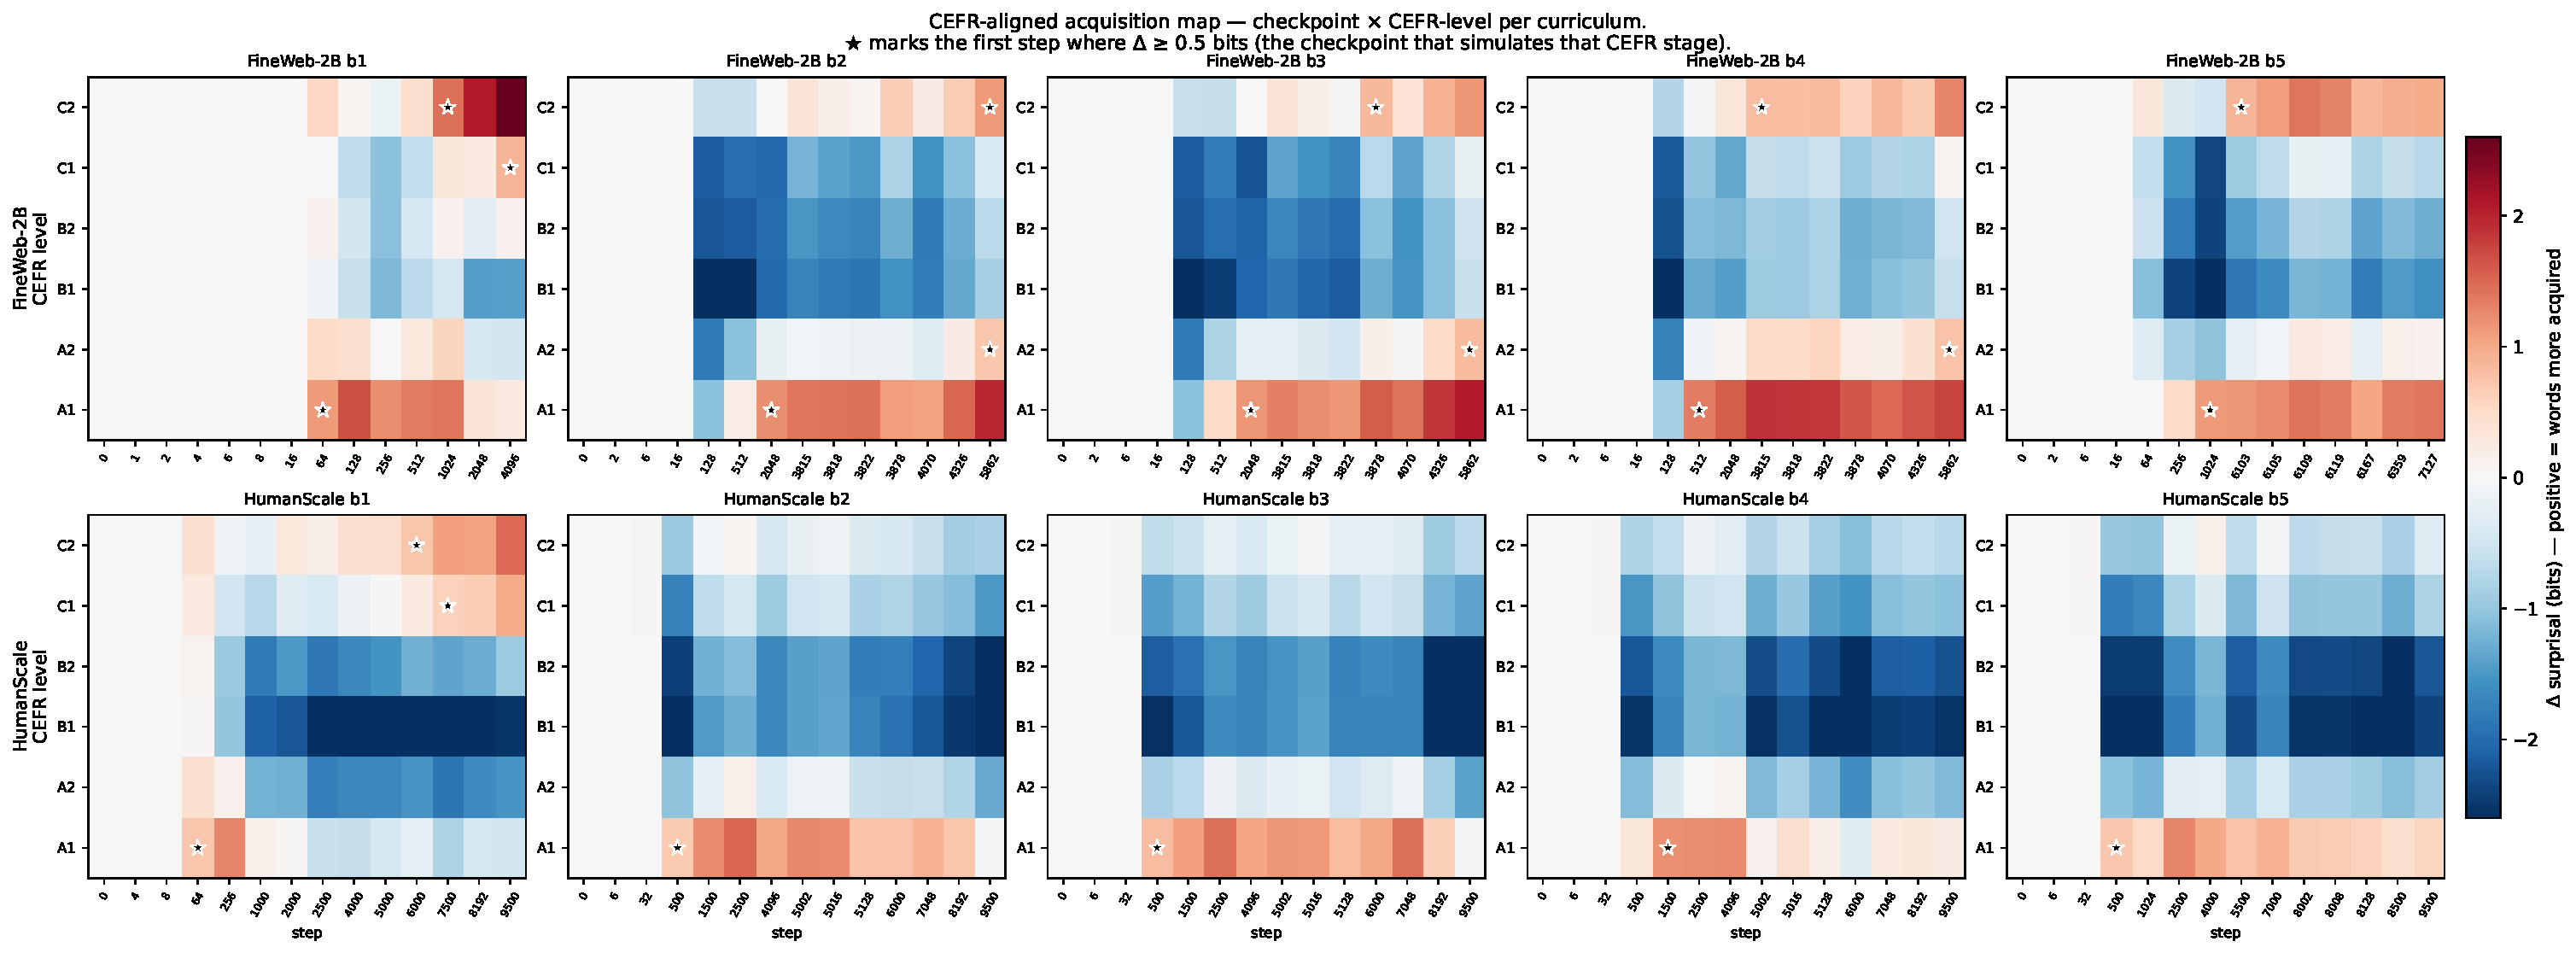
\includegraphics[width=0.86\linewidth,height=0.78\textheight,keepaspectratio]{fig/trajectory_cefr_alignment_heatmap.pdf}
  \caption{CEFR alignment heatmap: levels A1--C2 against log-spaced training step for the B3-33 nld--eng \textsc{Beetle} run.}
  \label{appcomp:trajectory_cefr_alignment_heatmap}
\end{figure}

\begin{figure}[!htbp]
  \centering
  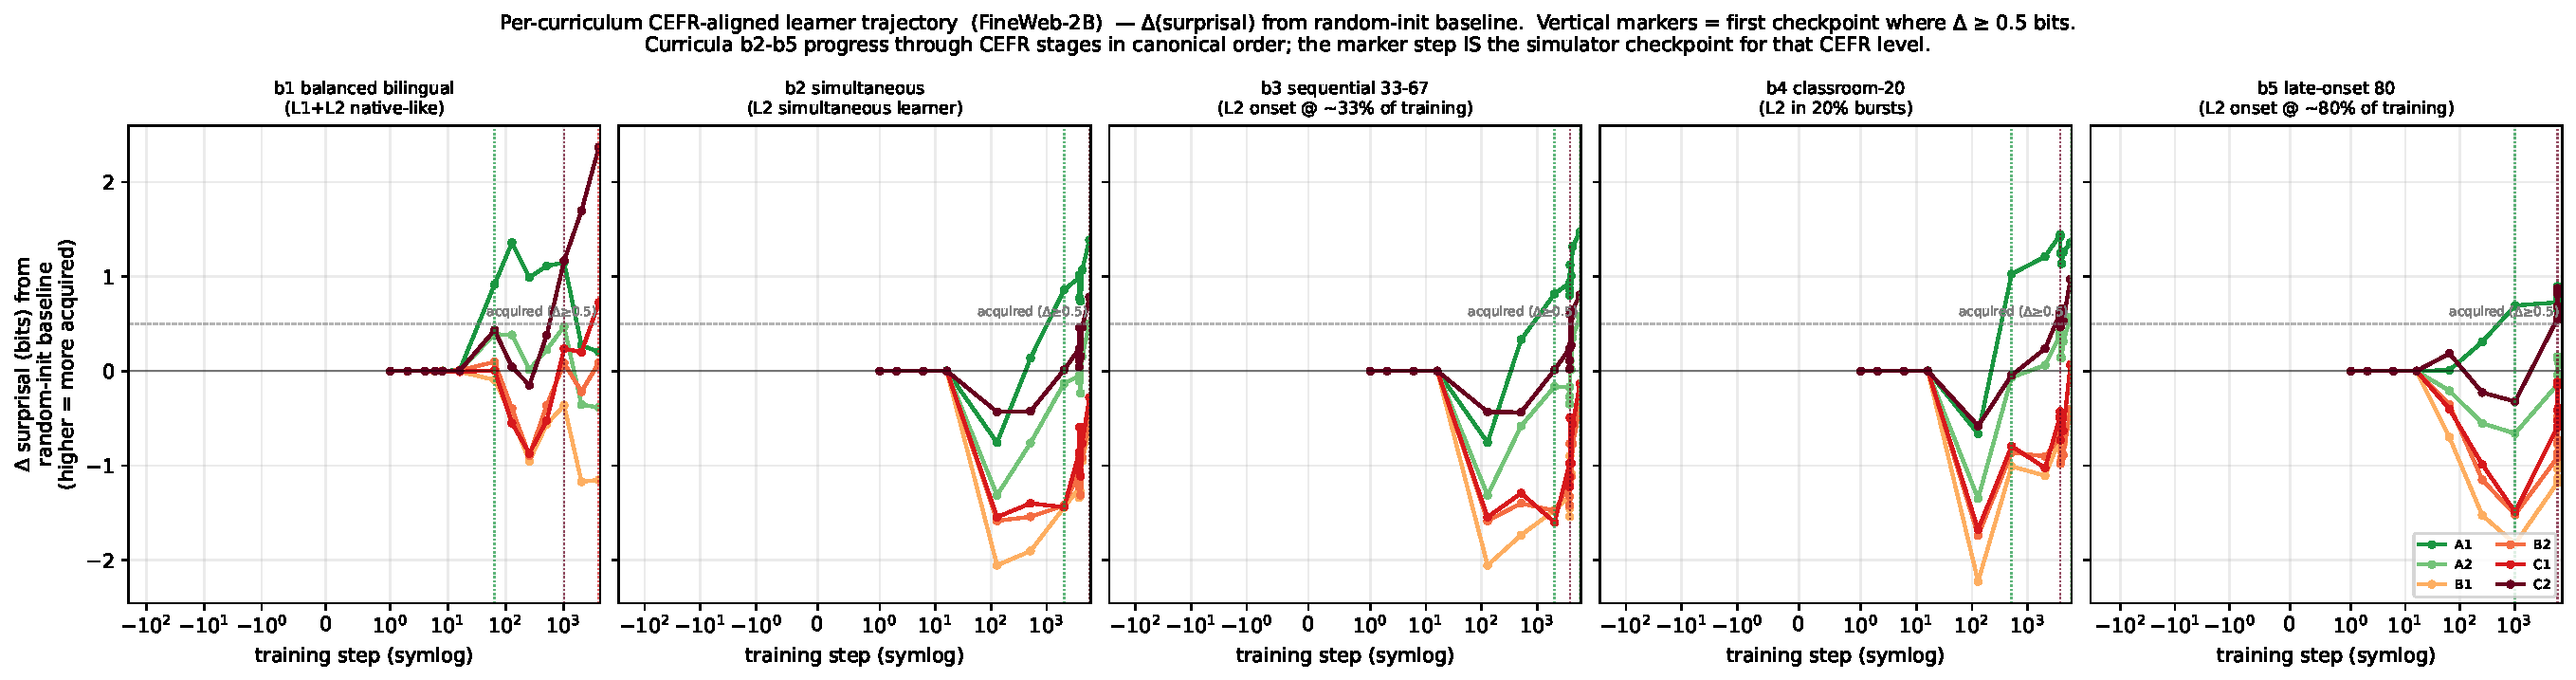
\includegraphics[width=0.86\linewidth,height=0.78\textheight,keepaspectratio]{fig/trajectory_cefr_fineweb2b.pdf}
  \caption{CEFR alignment trajectory at the \textsc{FineWeb}~2B token budget for \textsc{Beetle} curricula.}
  \label{appcomp:trajectory_cefr_fineweb2b}
\end{figure}

\begin{figure}[!htbp]
  \centering
  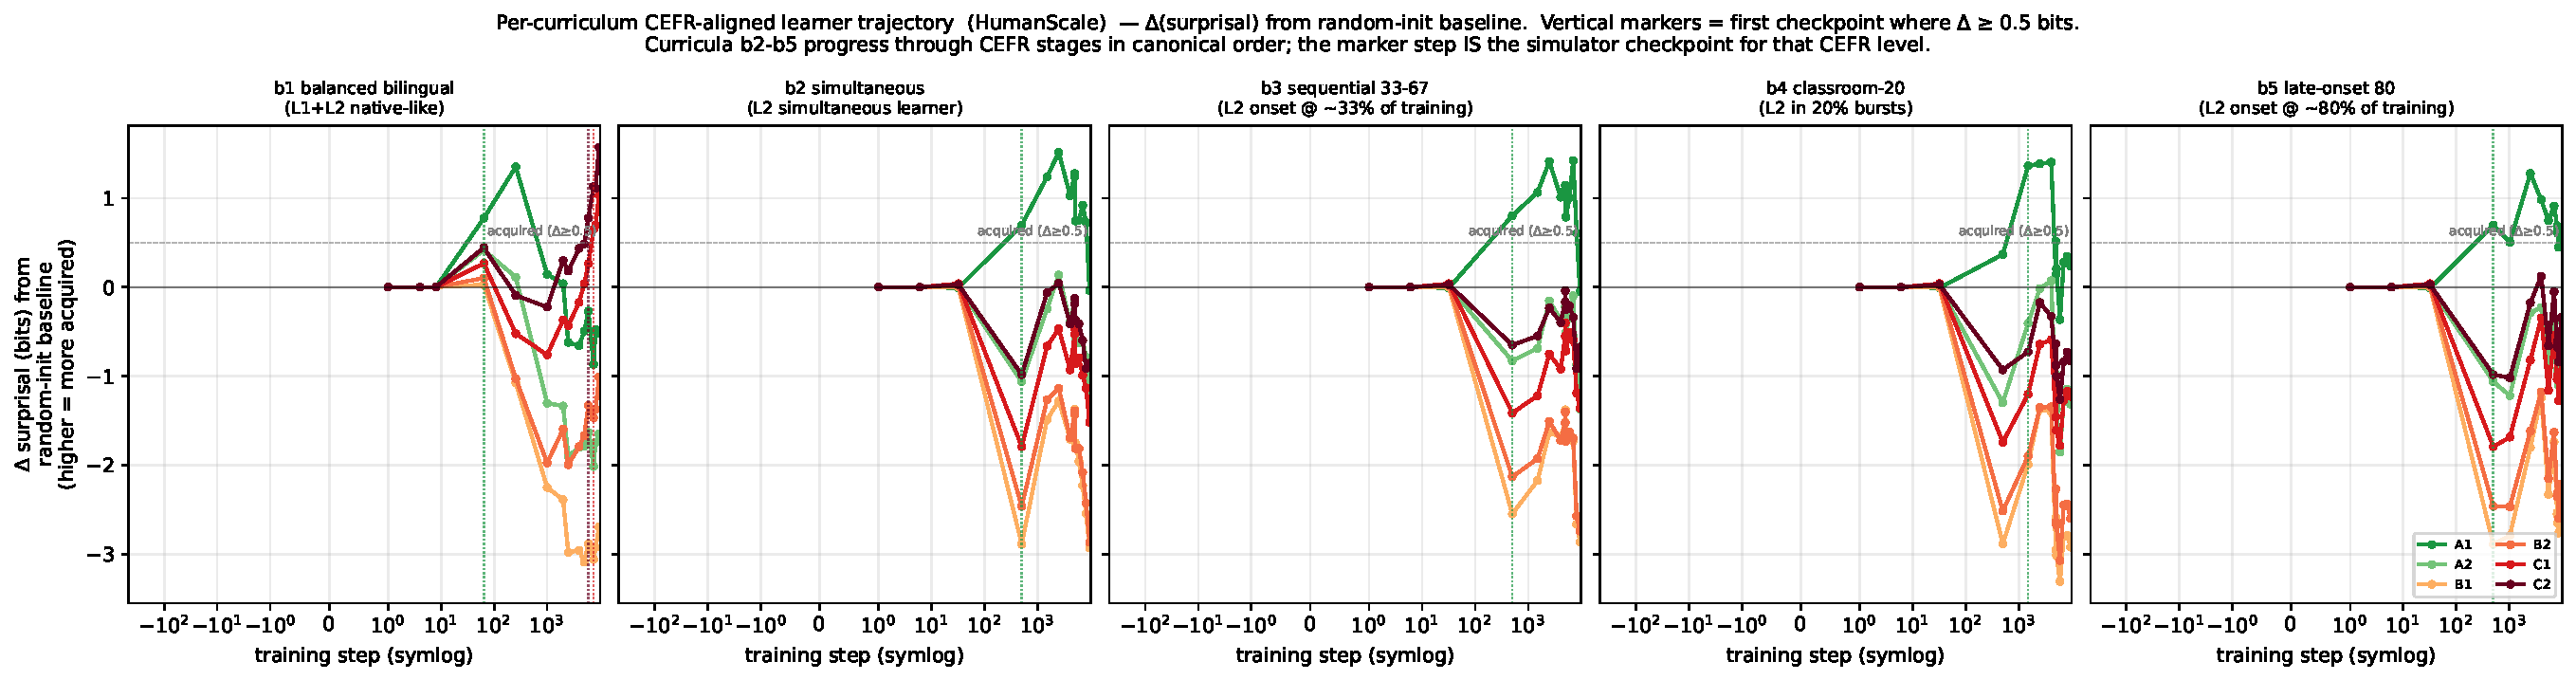
\includegraphics[width=0.86\linewidth,height=0.78\textheight,keepaspectratio]{fig/trajectory_cefr_humanscale.pdf}
  \caption{CEFR alignment trajectory at the \textsc{HumanScale}~100M token budget for \textsc{Beetle} curricula.}
  \label{appcomp:trajectory_cefr_humanscale}
\end{figure}

\newpage
\section{Comparison of Continual Learning Strategies}

\begin{figure*}[!ht]
    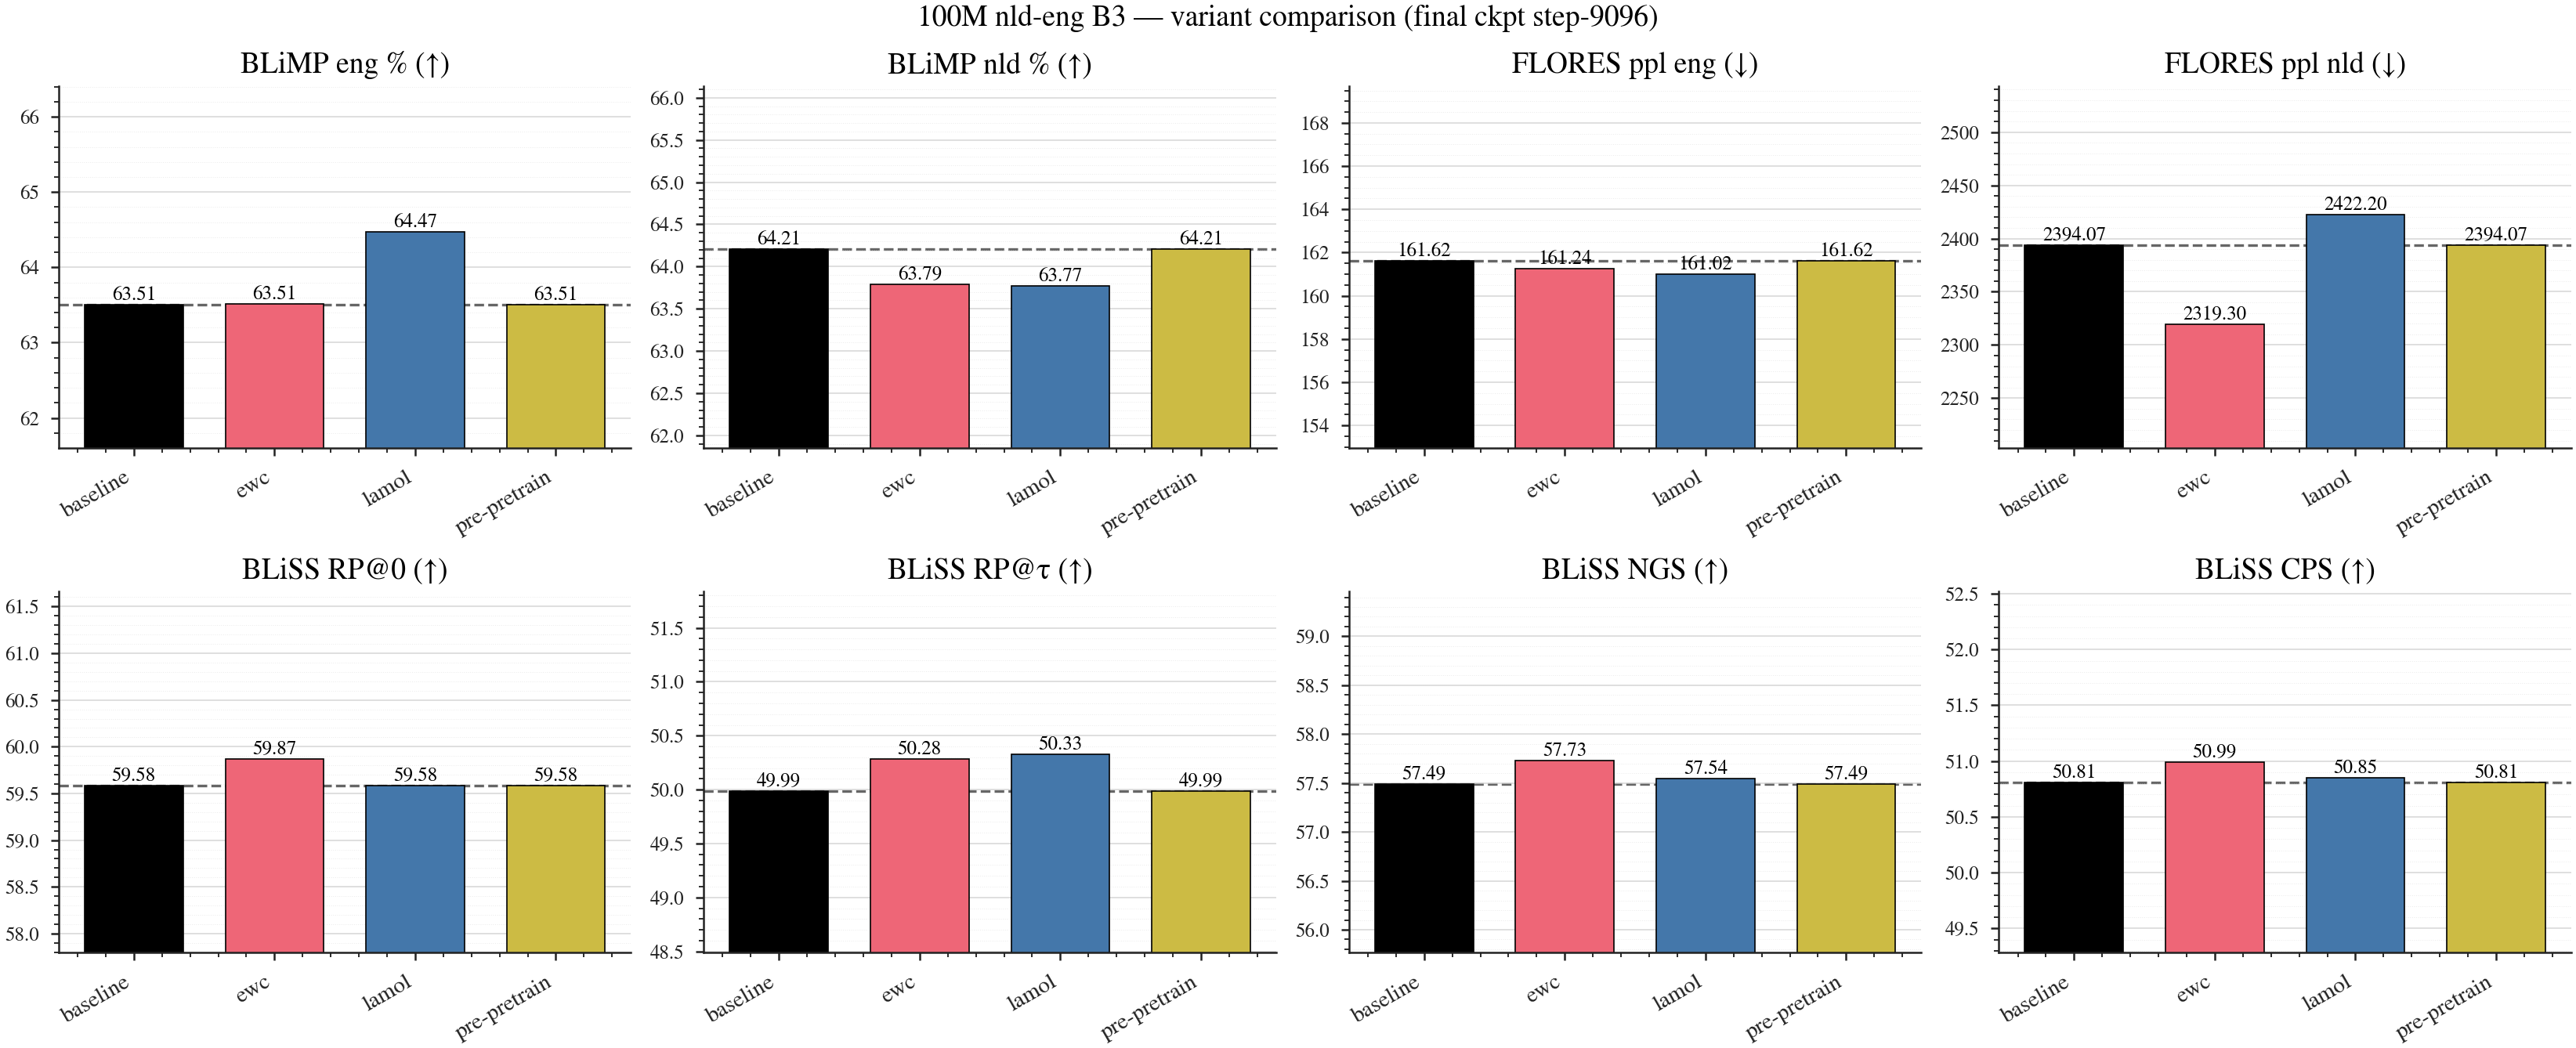
\includegraphics[width=0.86\linewidth,height=0.78\textheight,keepaspectratio]{fig/fig_variant_comparison_100m.png}
\end{figure*}


\end{document}

